\documentclass[11pt]{beamer}
\usetheme{Luebeck}
\usepackage[utf8]{inputenc}
\usepackage[english]{babel}
\usepackage{amsmath}
\usepackage{siunitx}
\usepackage{amsfonts}
\usepackage{amssymb}
\usepackage{graphicx}
\usepackage{booktabs}
\usepackage{subcaption}
\author{Eugenia Spedicato, Lina Maria Ortiz Parra, Jonah Blank}
\title{Detector induced assymetry in CP violation measurements}
%\setbeamercovered{transparent}
%\setbeamertemplate{navigation symbols}{}
%\logo{}
%\institute{}
%\date{}
%\subject{}
\begin{document}

\begin{frame}
\titlepage
\end{frame}

%\begin{frame}
%\tableofcontents
%\end{frame}

\begin{frame}{Comments - efficiencies}
\begin{itemize}
\item very small errors in $D=\frac{\epsilon_+ - \epsilon_-}{\epsilon_+ + \epsilon_-}$\\
$\rightarrow$ $D=0$ out of $5\sigma$-range
\item smaller error for $UP$-polarity due to higher statistics
\item no difference between $UP$ and $DOWN$ within scope of the error
\item in the MC: $\epsilon_{D^*}=0$(\texttt{Dst\char`_reconstructed} always 0)\\
in our computation: $\epsilon_{D^*}=\epsilon_{\pi,s}\cdot\epsilon_{D^0}$
\end{itemize}
\end{frame}
\begin{frame}{Comments - plots}
\begin{itemize}
\item structure of $\epsilon(\phi)$ probably due to rectangular detector shape
\item peak in $\epsilon_{D^*}(\theta)$ within scope of error
\end{itemize}
\end{frame}
\begin{frame}
\begin{LARGE}
\textbf{Total}
\end{LARGE}
\end{frame}
\begin{frame}{Efficiencies}
\begin{table}
\resizebox{\textwidth}{!}{
	\begin{tabular}{cS[table-format=2.2]@{${}\pm{}$}S[table-format=1.2]S[table-format=2.2]@{${}\pm{}$}S[table-format=1.2]S[table-format=2.2]@{${}\pm{}$}S[table-format=1.2]S[table-format=2.2]@{${}\pm{}$}S[table-format=1.2]S[table-format=2.2]@{${}\pm{}$}S[table-format=1.2]}
		\toprule
		{Polarity} & \multicolumn{2}{c}{$\epsilon_{\pi} $} & \multicolumn{2}{c}{$\epsilon_{K} $} & \multicolumn{2}{c}{$ \epsilon_{\pi,s} $} & \multicolumn{2}{c}{$\epsilon_{D^0} $} & \multicolumn{2}{c}{$\epsilon_{D^*} $} \\
		\midrule
		$UP$ & 86.61 & 0.04 & 84.65 & 0.04 & 76.61 & 0.05 & 73.33 & 0.05 & 56.26 & 0.06\\
		$DOWN$ & 86.61 & 0.04 & 84.67 & 0.05 & 76.54 & 0.06 & 73.33 & 0.06 & 56.23 & 0.07\\
		\bottomrule
	\end{tabular}}
\end{table}
\end{frame}
\begin{frame}{$\pi$-efficiency}
\begin{figure}
\begin{subfigure}{0.45\textwidth}
\includegraphics[width=0.9\textwidth]{up_pdf/single/tot/h_pt_reco_Pi.pdf}
\end{subfigure}
\begin{subfigure}{0.45\textwidth}
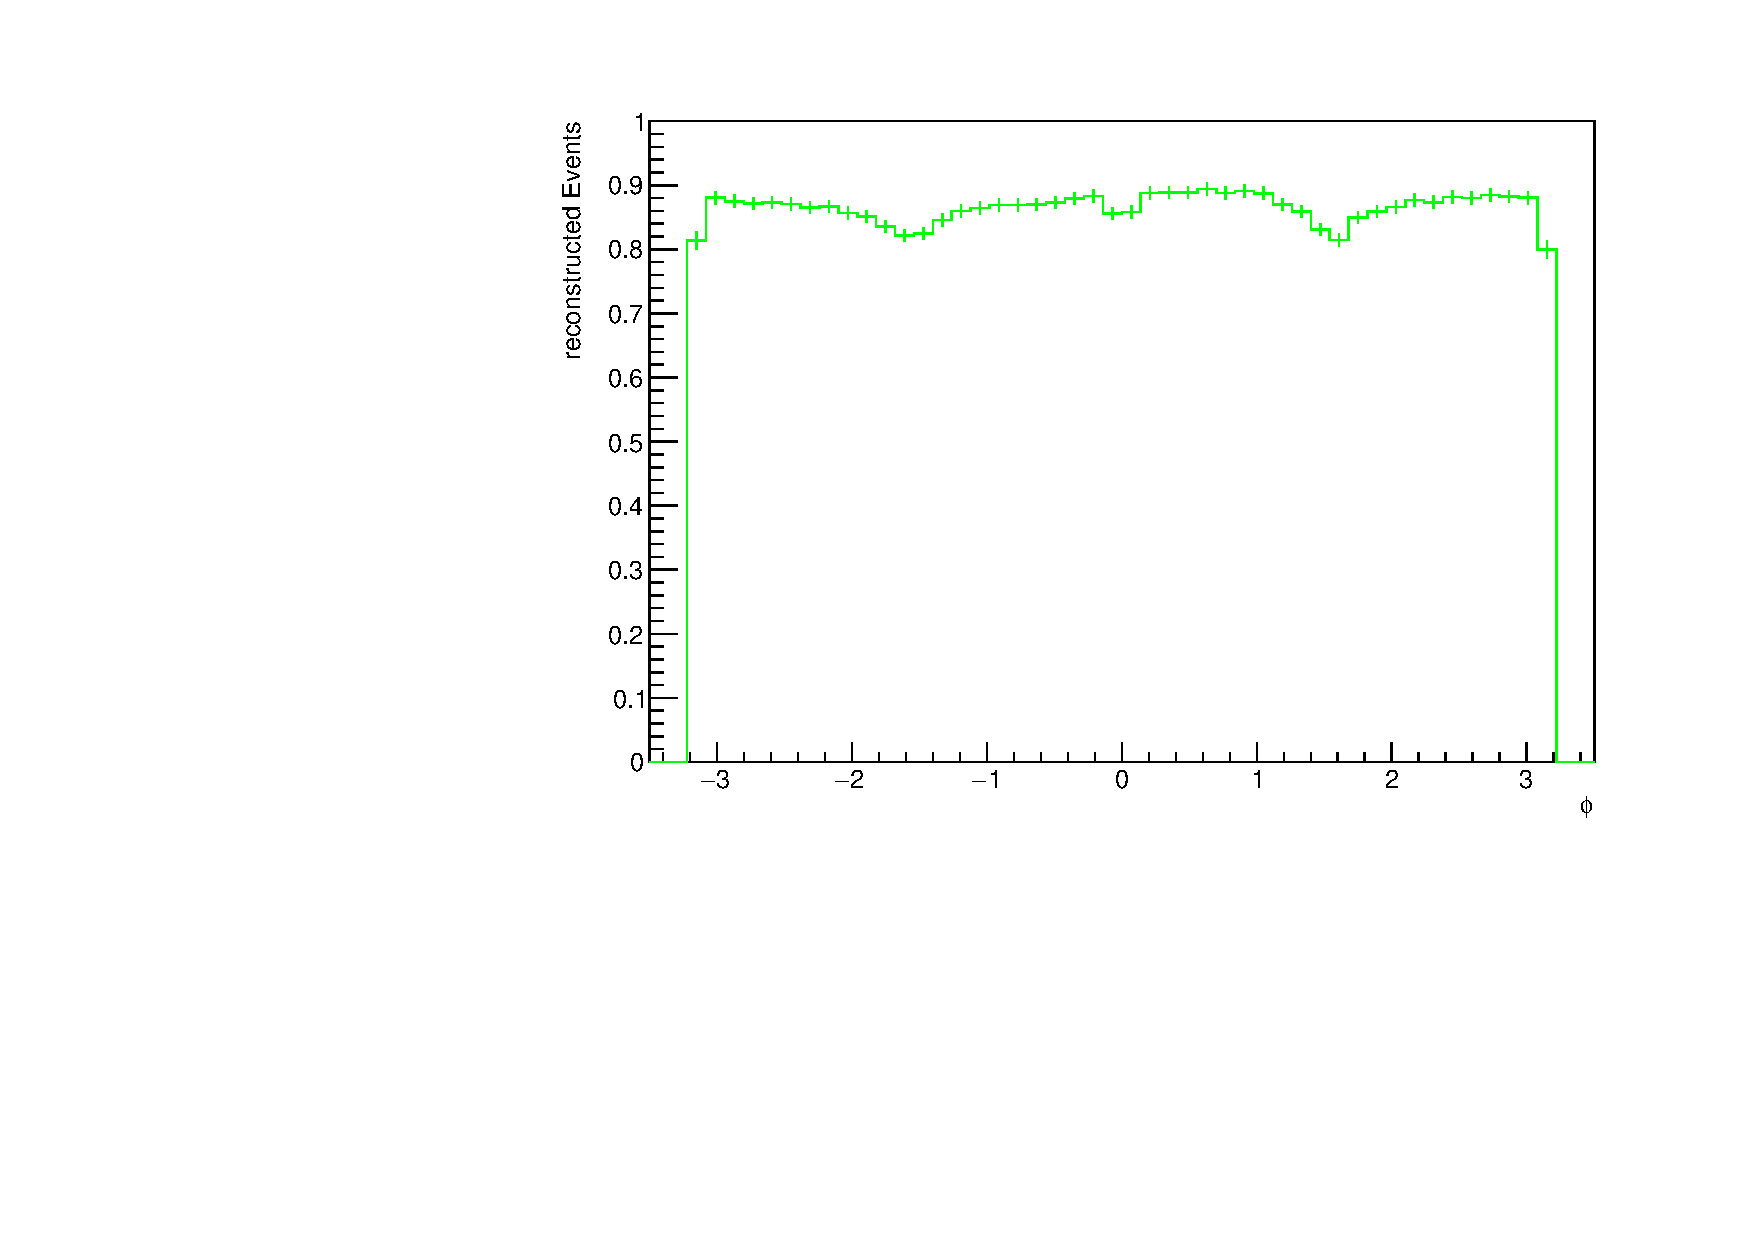
\includegraphics[width=0.9\textwidth]{up_pdf/single/tot/h_phi_reco_Pi.pdf}
\end{subfigure}
\begin{subfigure}{0.45\textwidth}
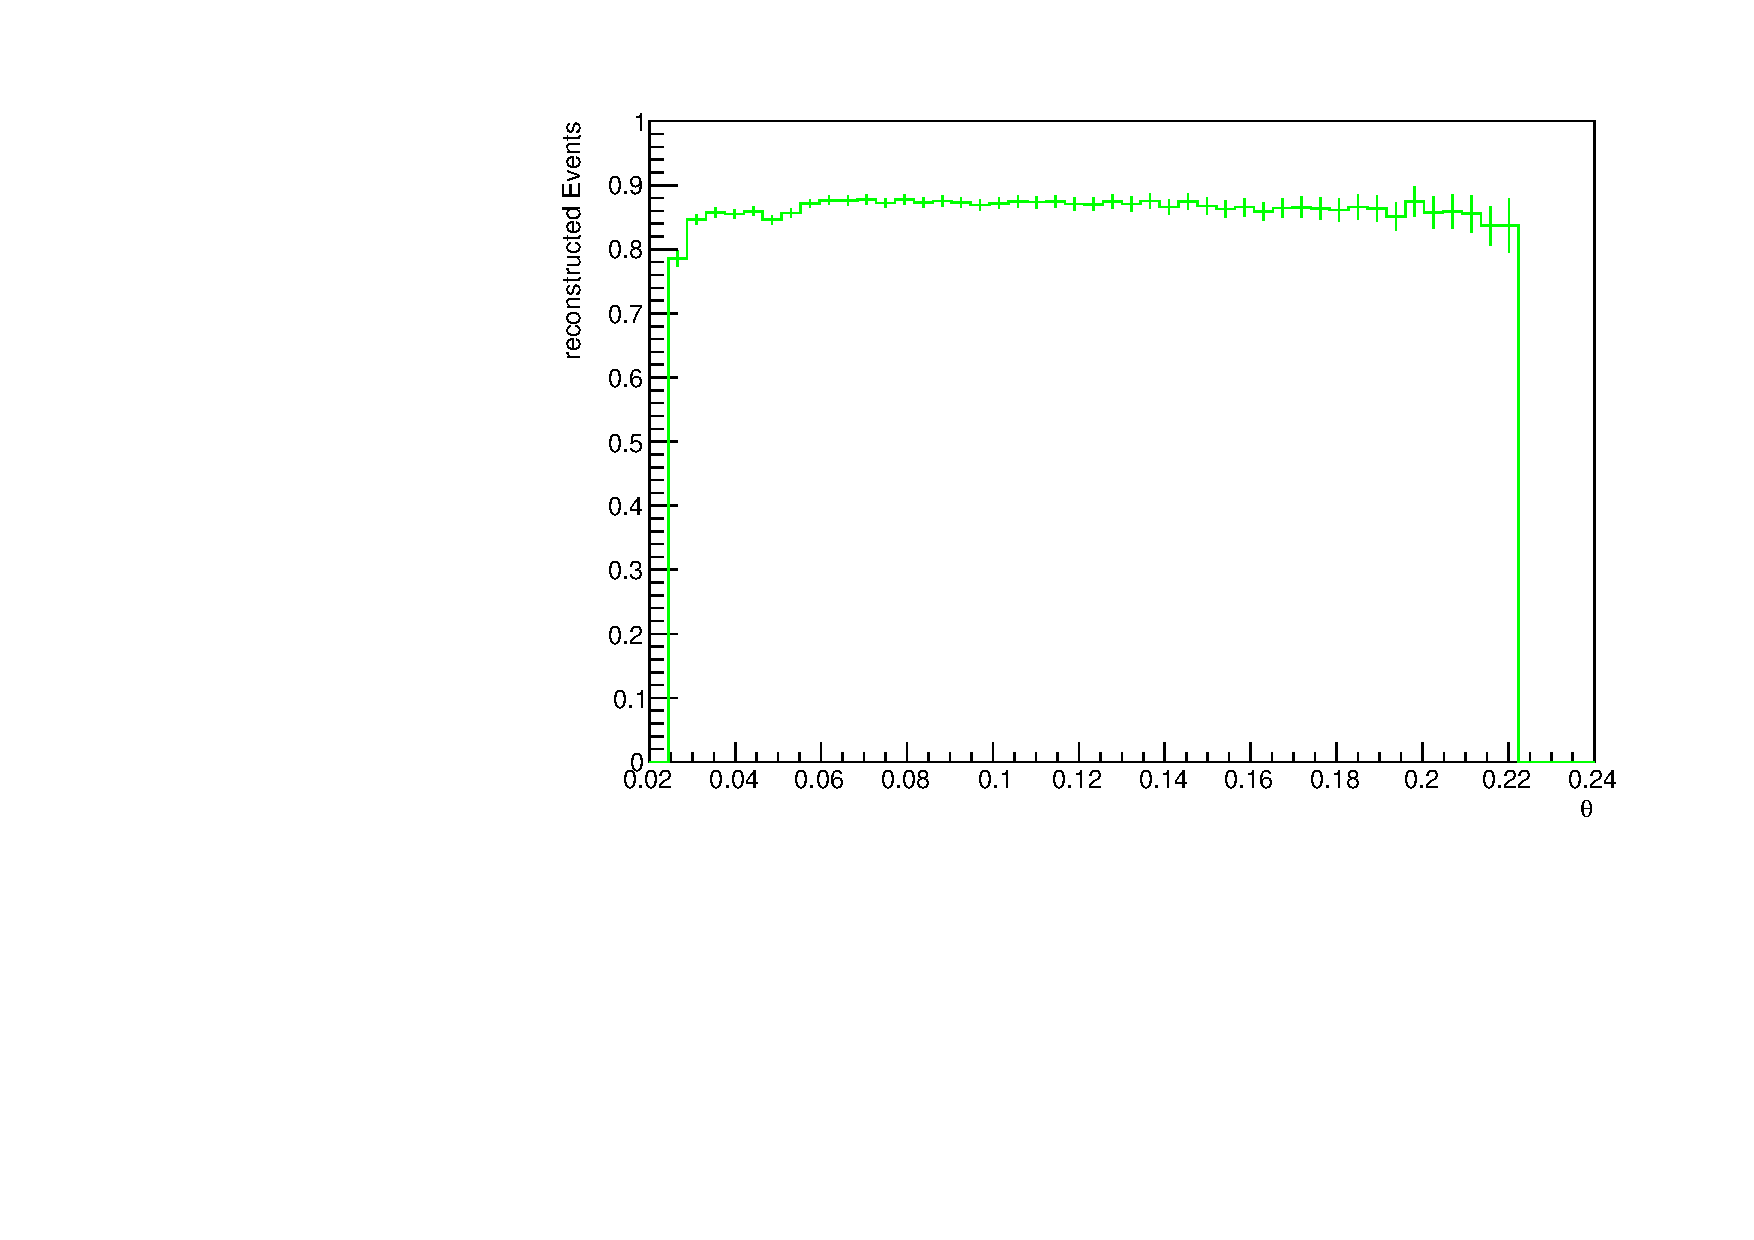
\includegraphics[width=0.9\textwidth]{up_pdf/single/tot/h_theta_reco_Pi.pdf}
\end{subfigure}
\begin{subfigure}{0.45\textwidth}
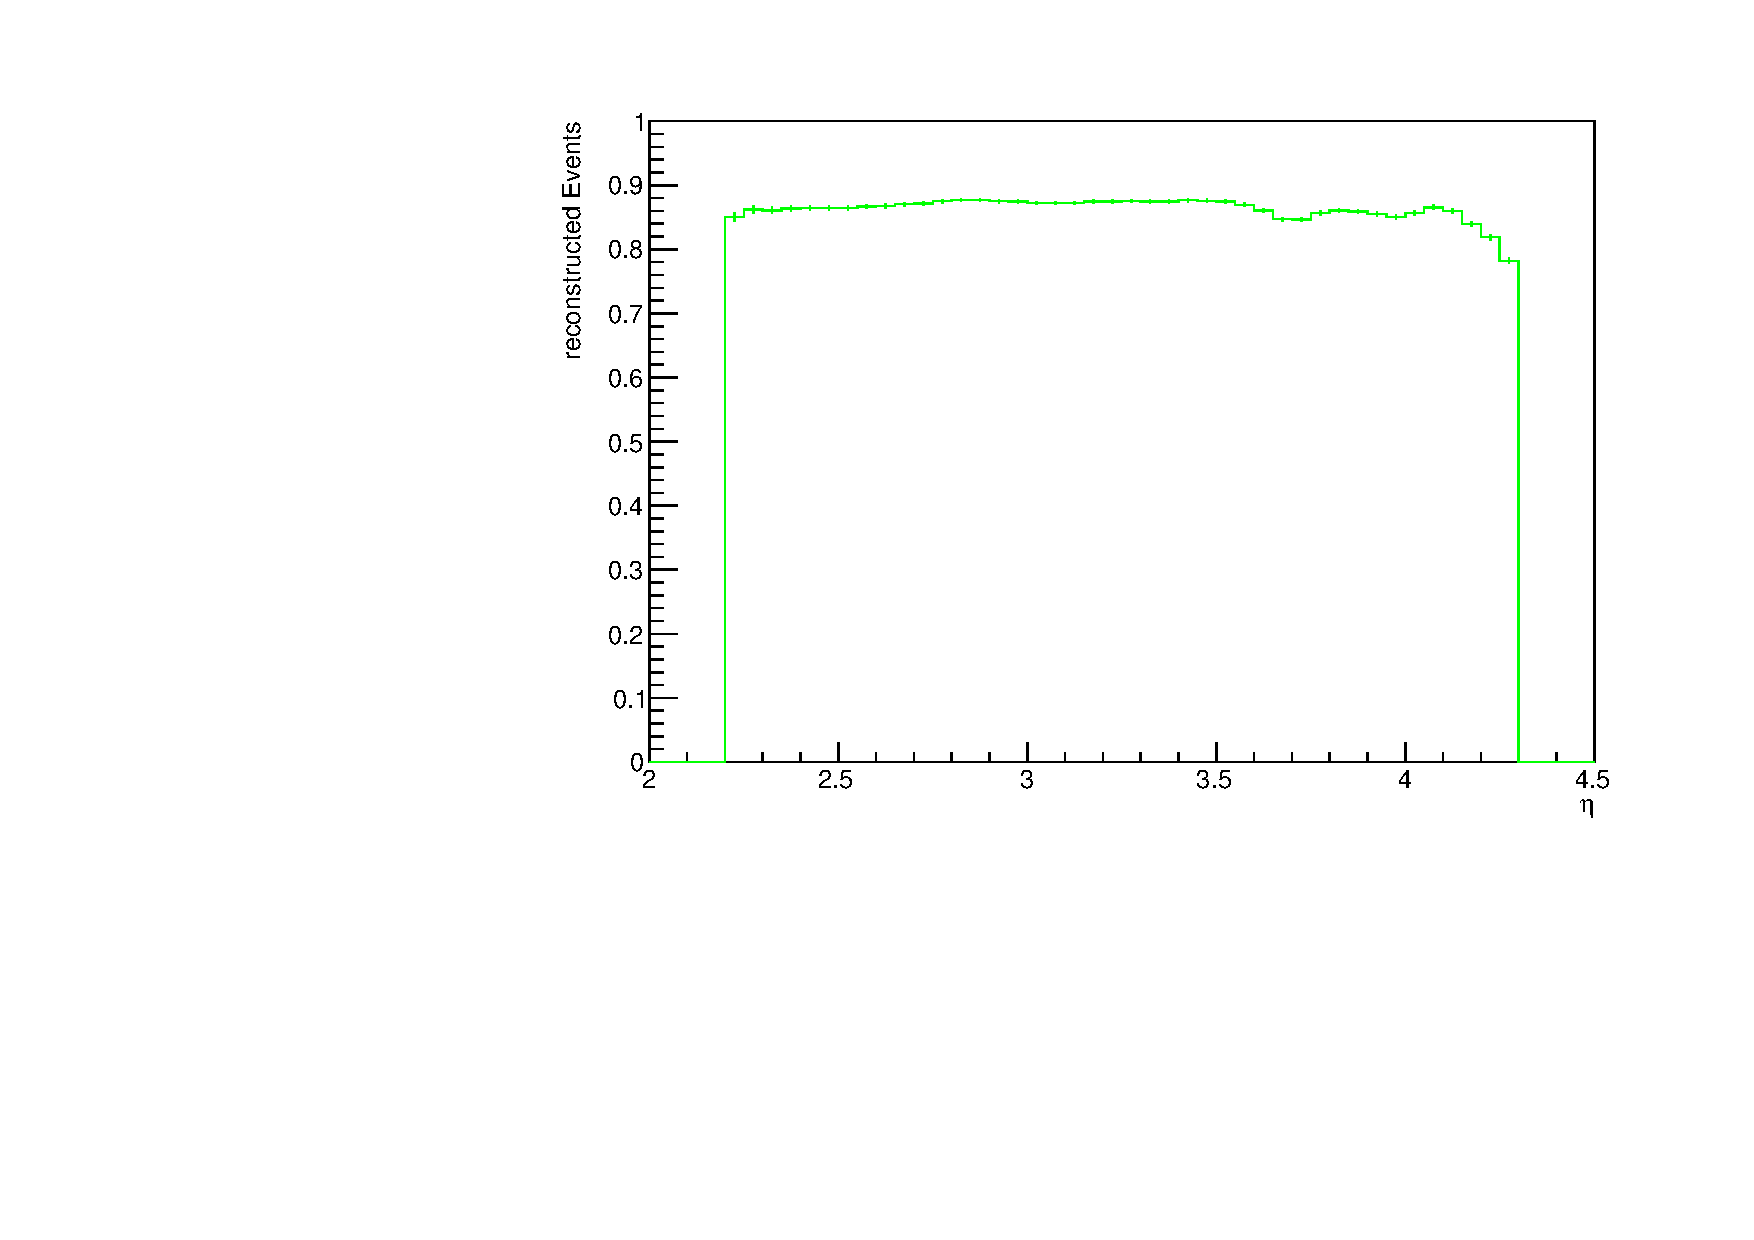
\includegraphics[width=0.9\textwidth]{up_pdf/single/tot/h_eta_reco_Pi.pdf}
\end{subfigure}
\end{figure}
\end{frame}
\begin{frame}{$K$-efficiency}
\begin{figure}
\begin{subfigure}{0.45\textwidth}
\includegraphics[width=0.9\textwidth]{up_pdf/single/tot/h_pt_reco_K.pdf}
\end{subfigure}
\begin{subfigure}{0.45\textwidth}
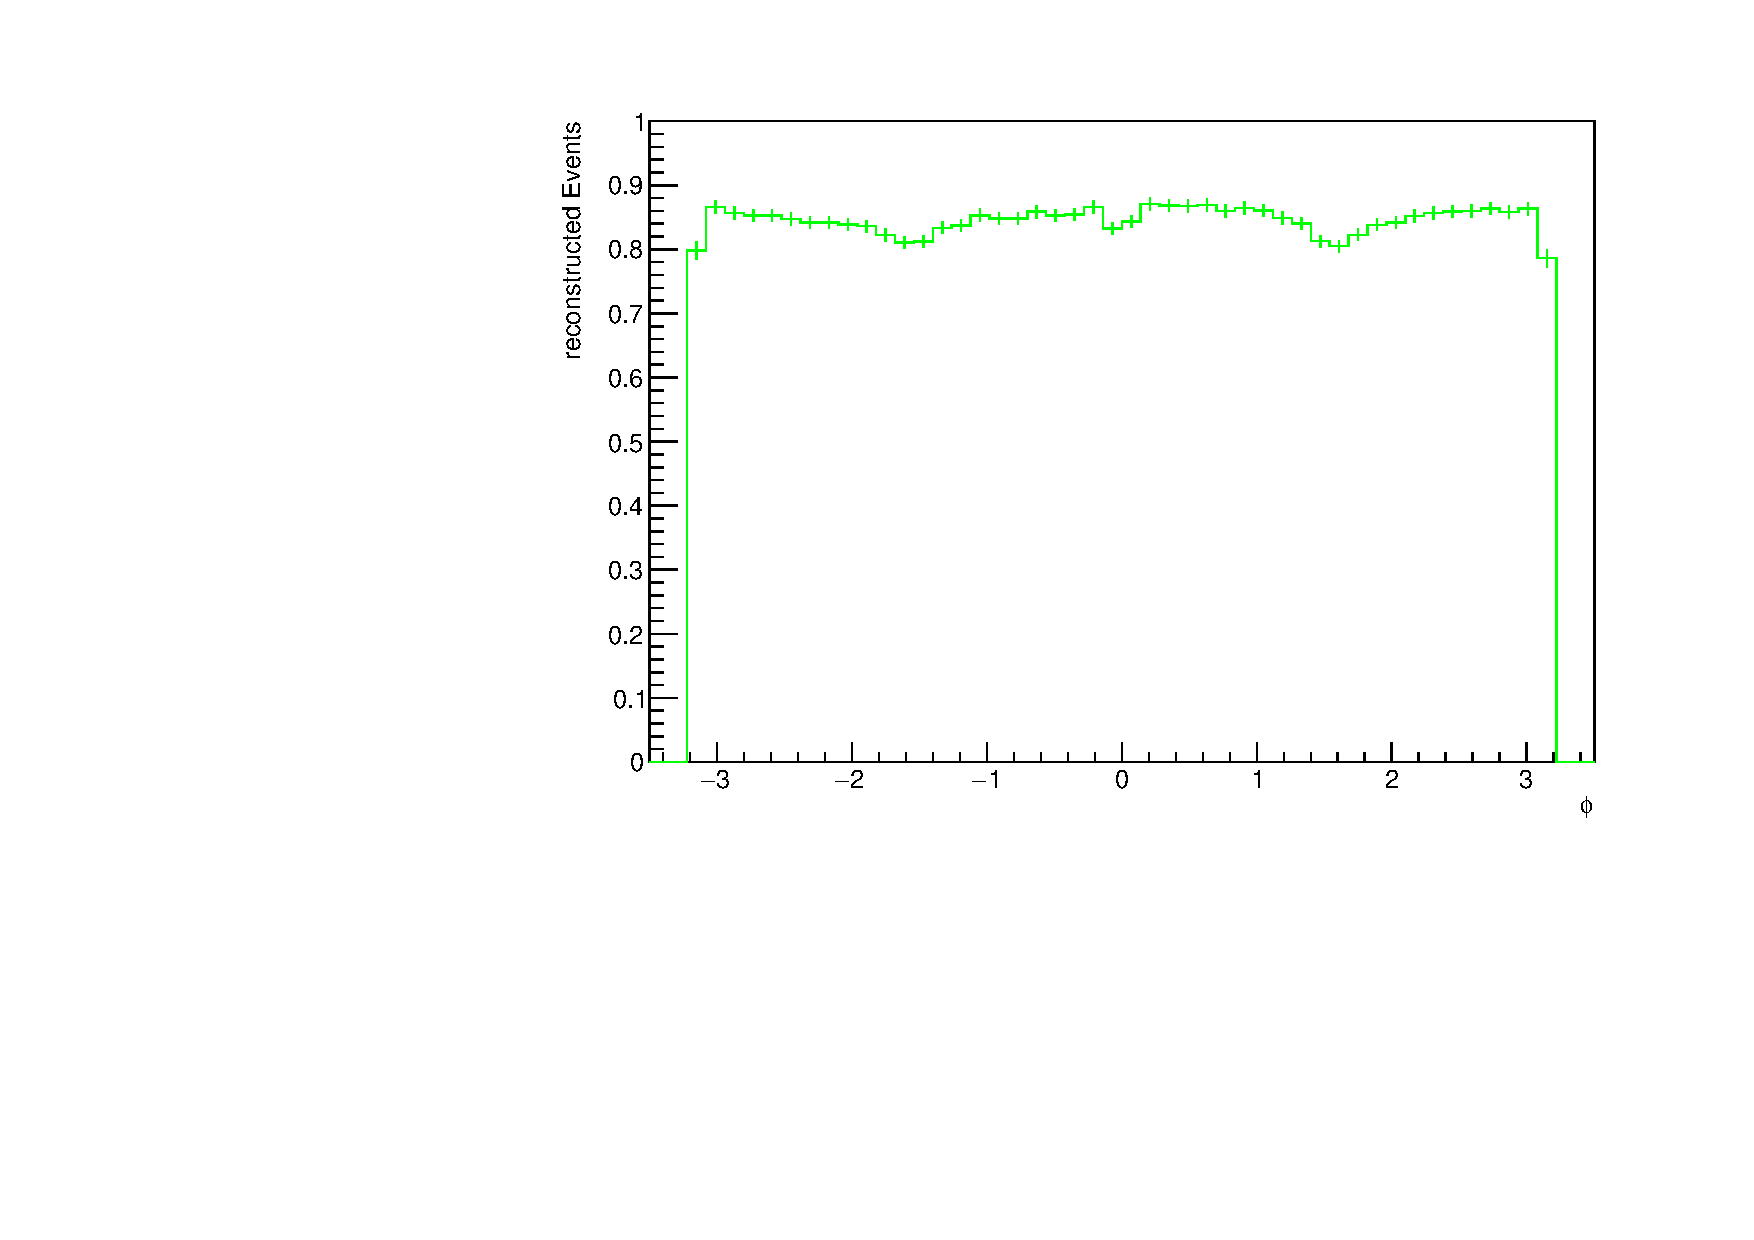
\includegraphics[width=0.9\textwidth]{up_pdf/single/tot/h_phi_reco_K.pdf}
\end{subfigure}
\begin{subfigure}{0.45\textwidth}
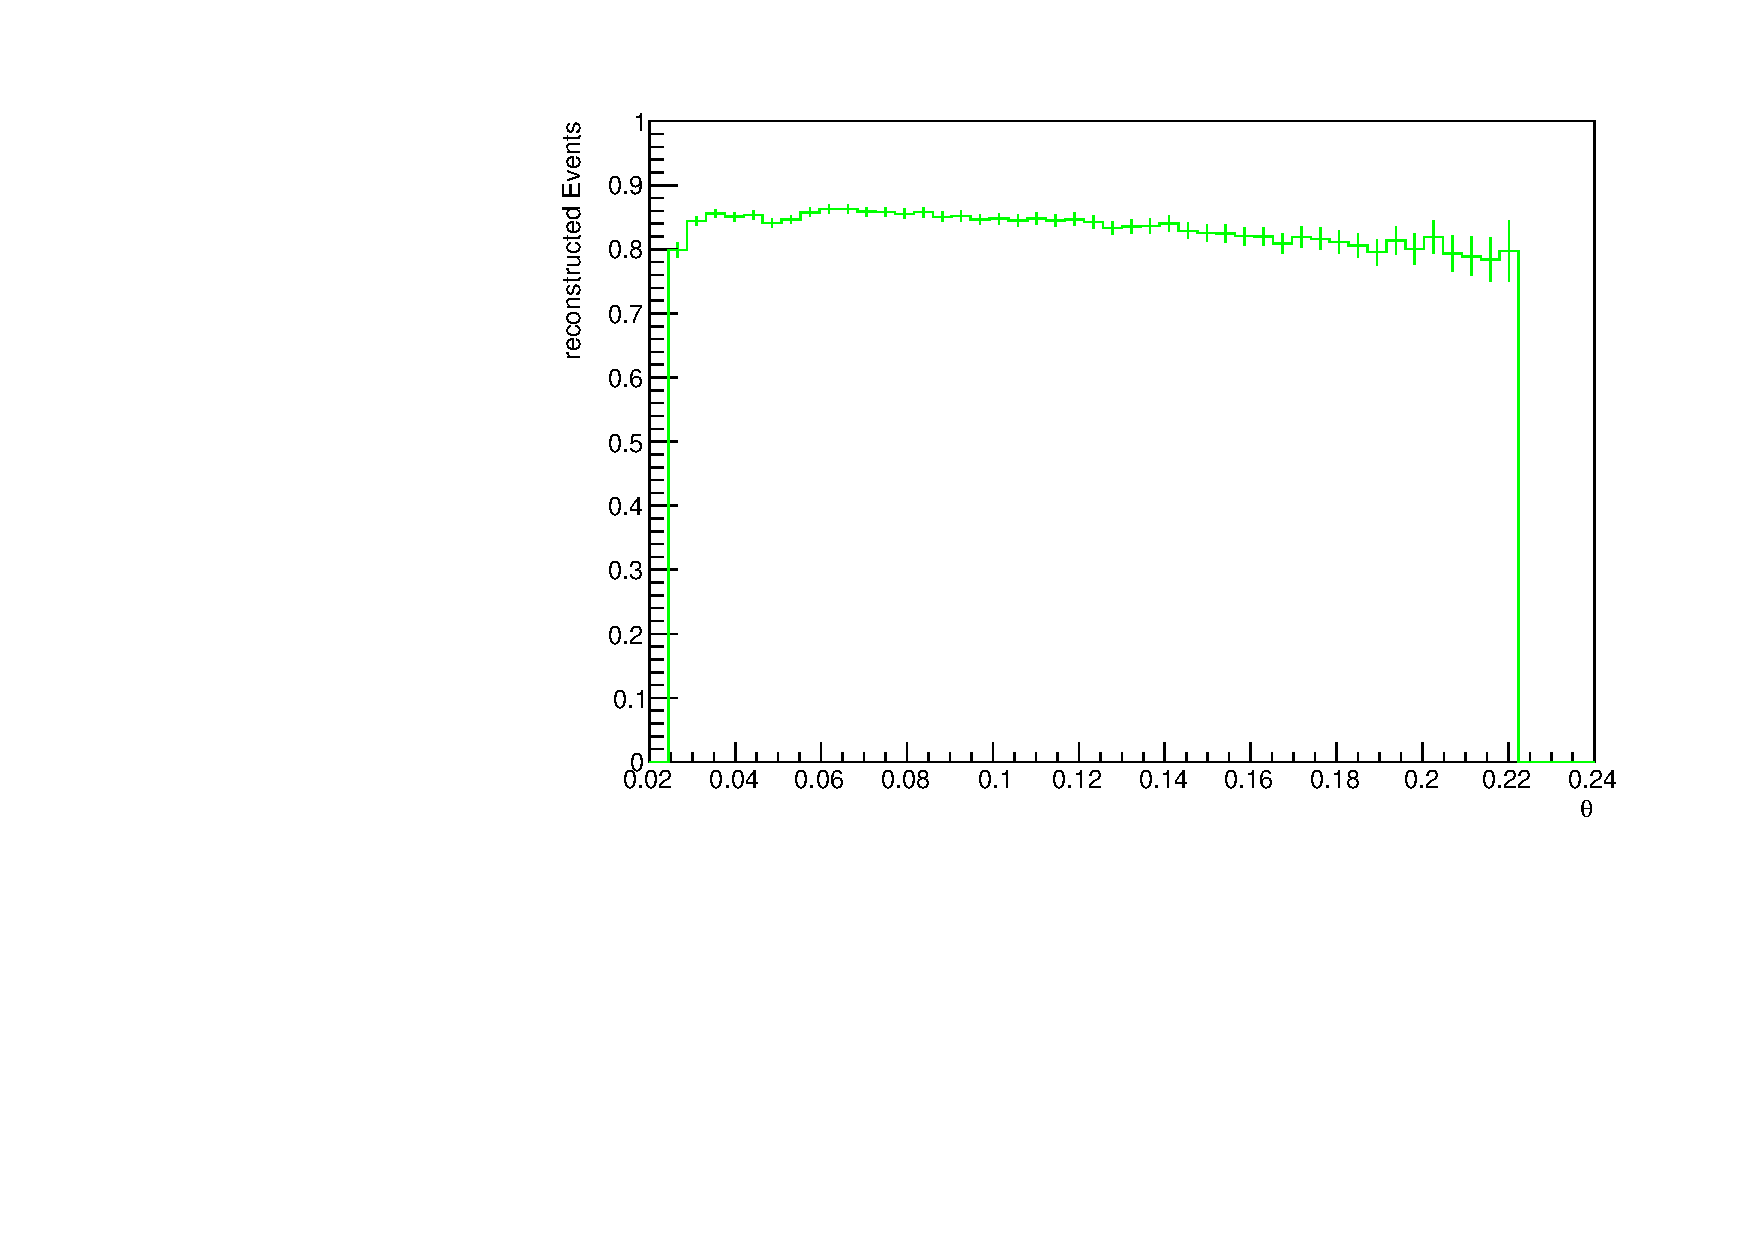
\includegraphics[width=0.9\textwidth]{up_pdf/single/tot/h_theta_reco_K.pdf}
\end{subfigure}
\begin{subfigure}{0.45\textwidth}
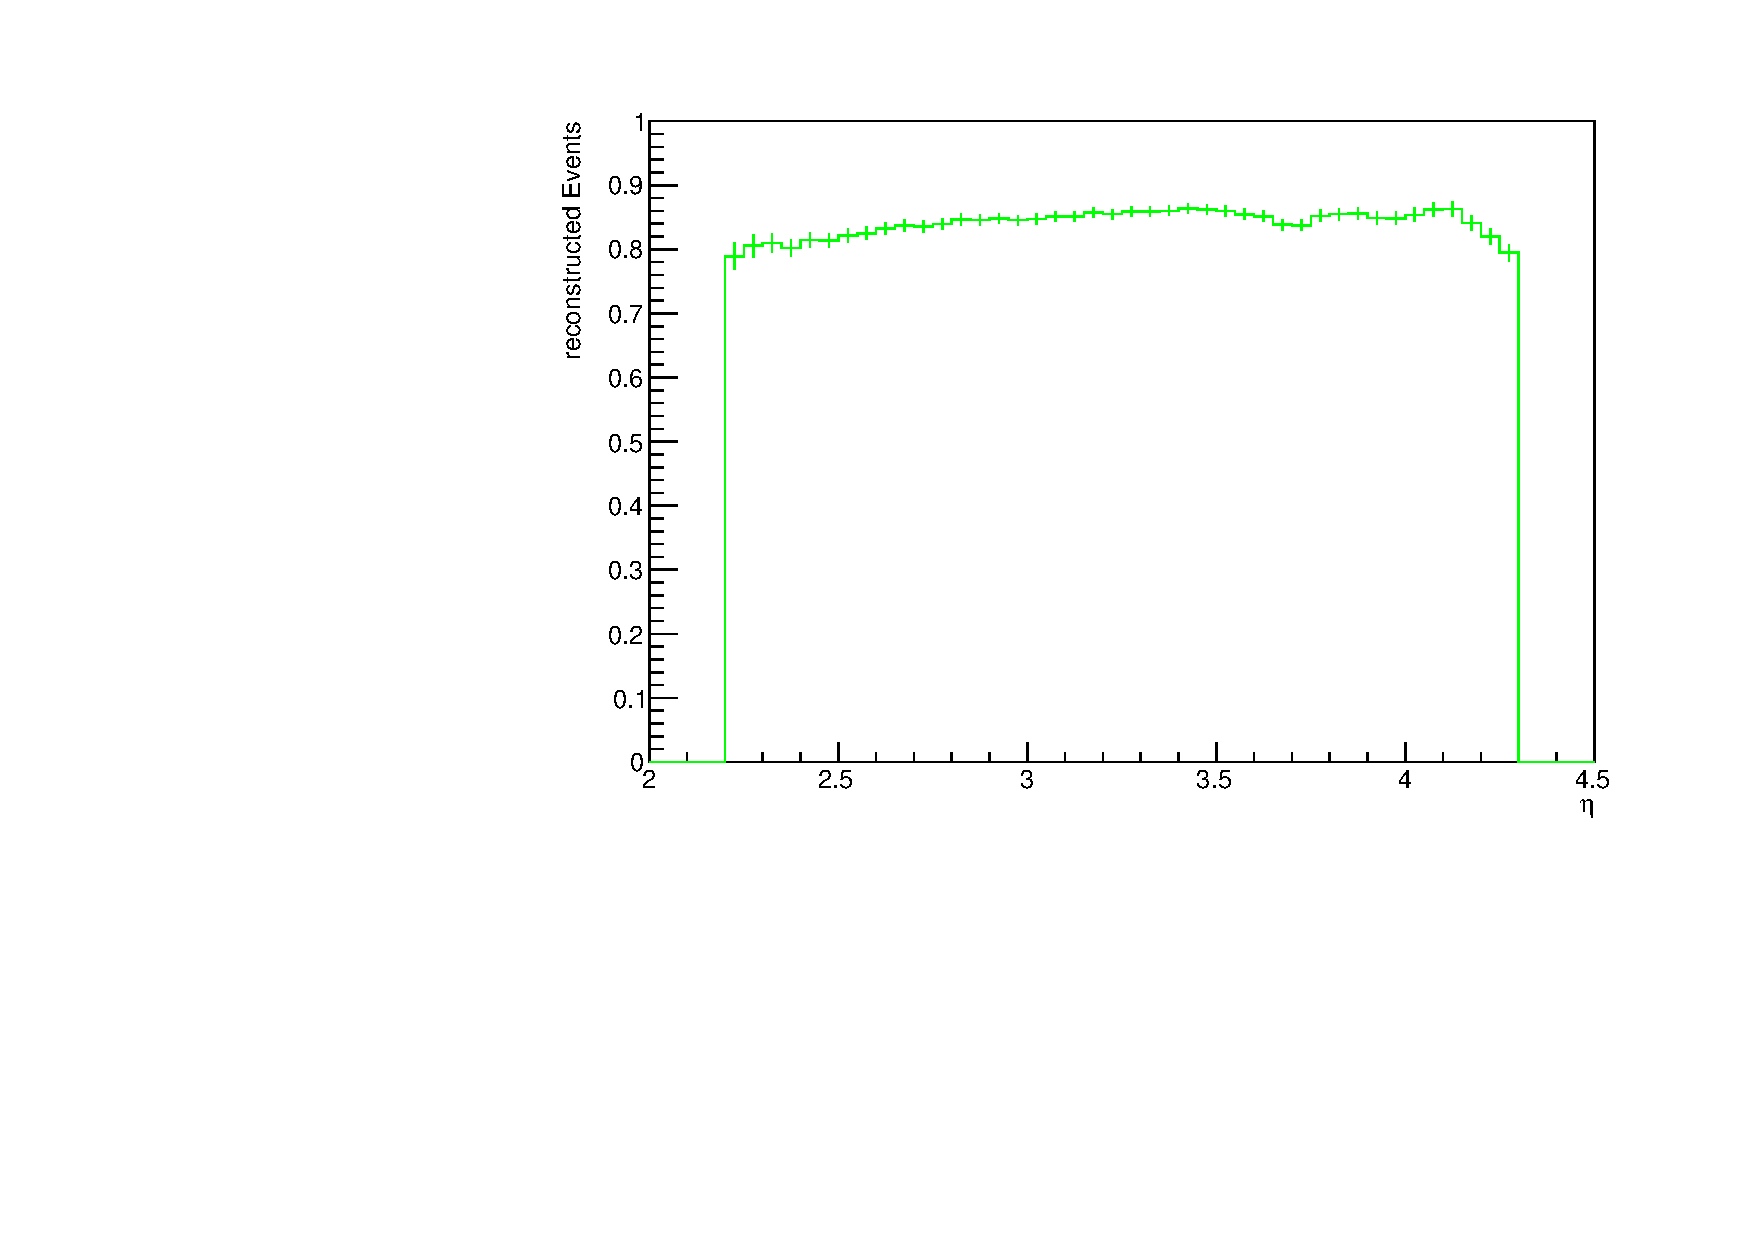
\includegraphics[width=0.9\textwidth]{up_pdf/single/tot/h_eta_reco_K.pdf}
\end{subfigure}
\end{figure}
\end{frame}
\begin{frame}{soft $\pi$-efficiency}
\begin{figure}
\begin{subfigure}{0.45\textwidth}
\includegraphics[width=0.9\textwidth]{up_pdf/single/tot/h_pt_reco_Dst.pdf}
\end{subfigure}
\begin{subfigure}{0.45\textwidth}
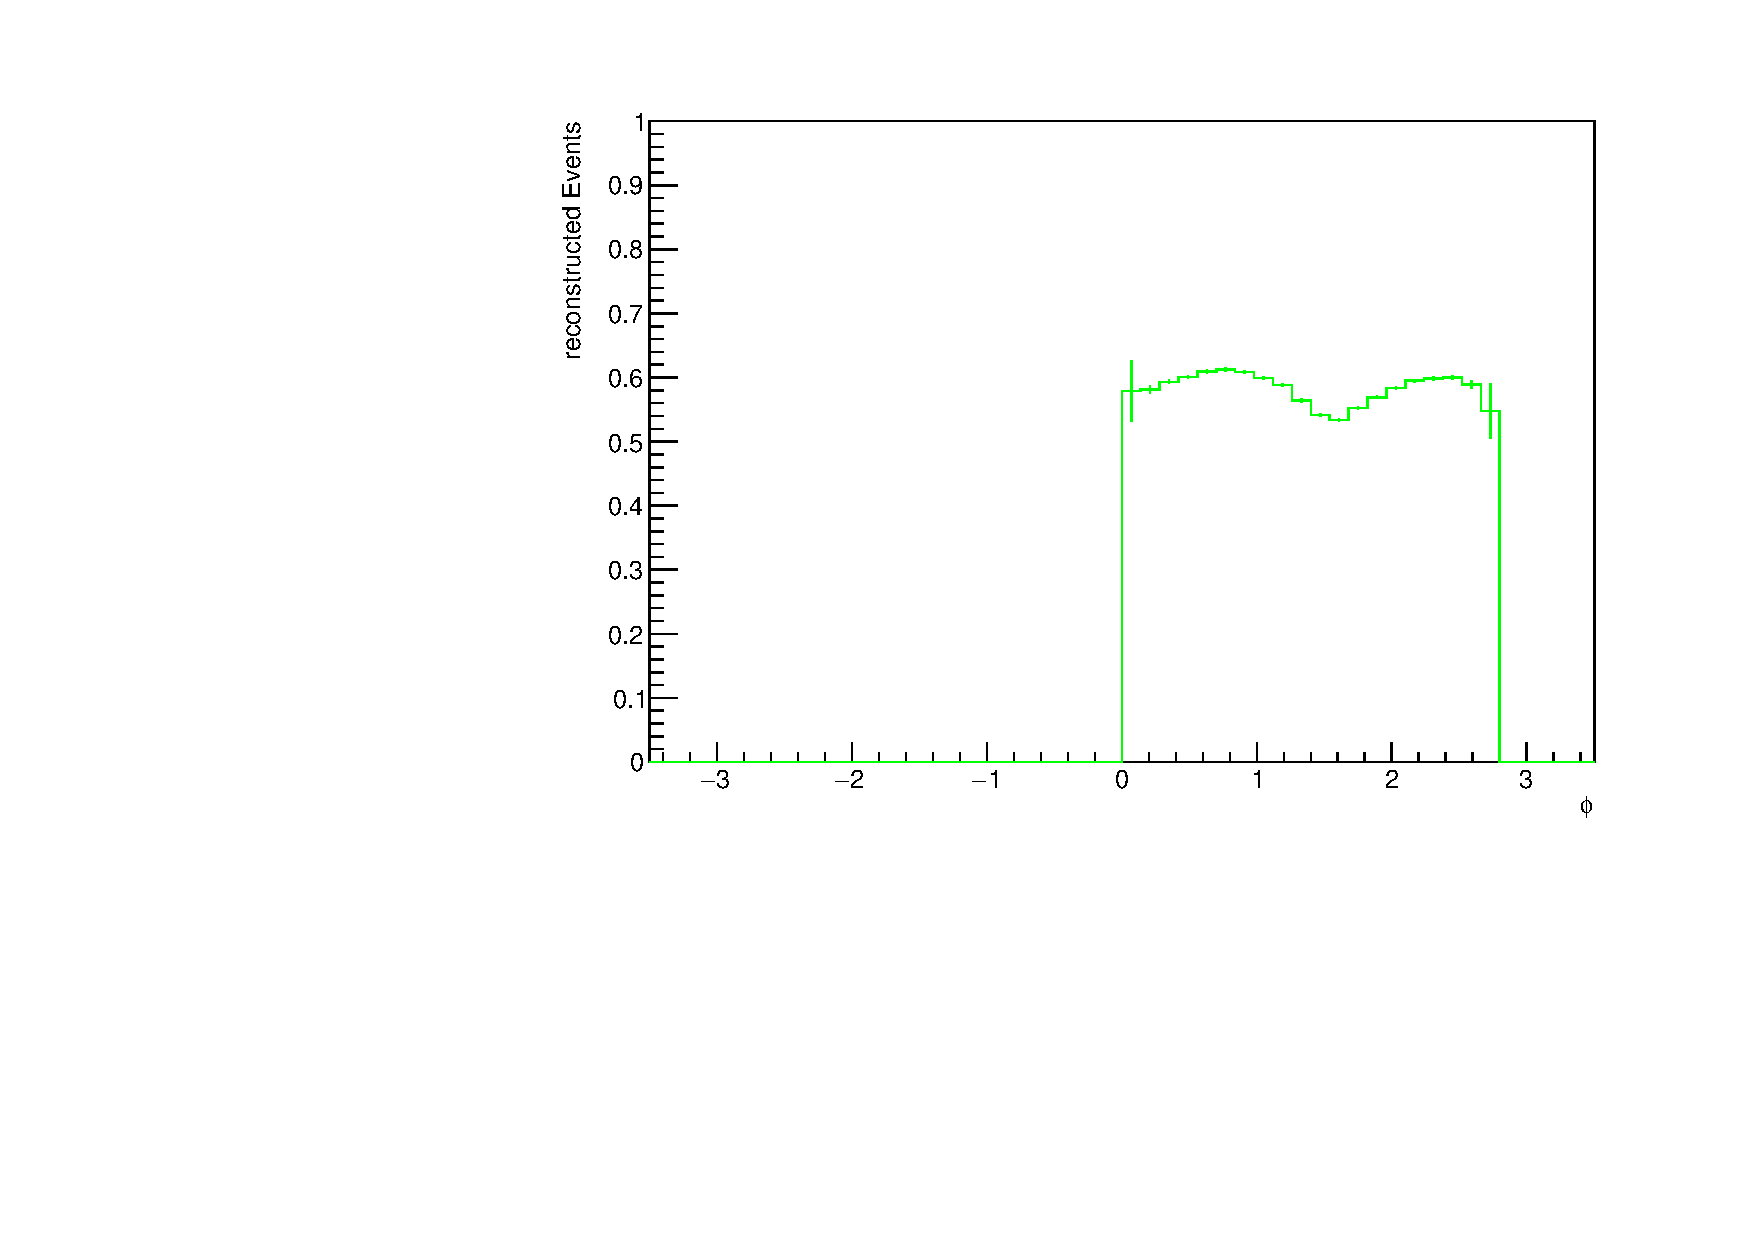
\includegraphics[width=0.9\textwidth]{up_pdf/single/tot/h_phi_reco_Dst.pdf}
\end{subfigure}
\begin{subfigure}{0.45\textwidth}
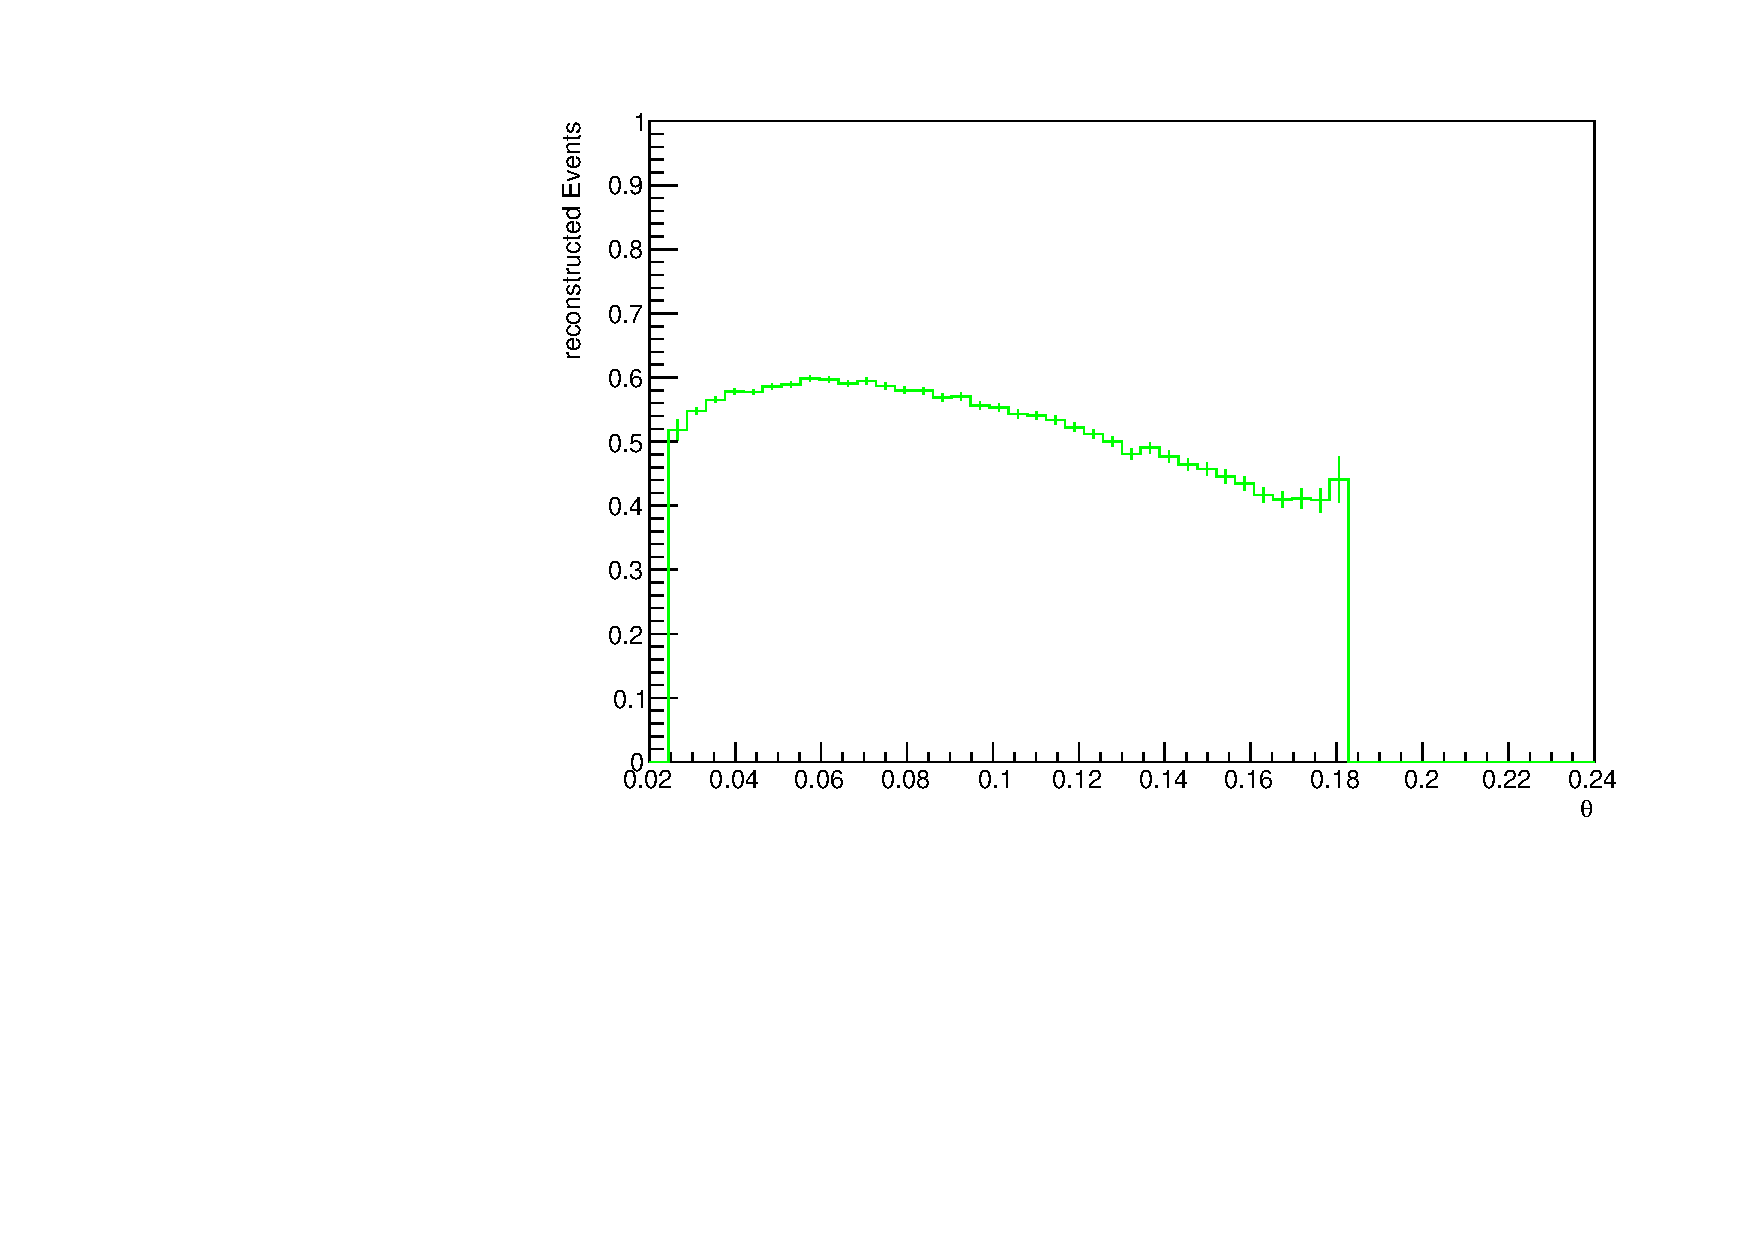
\includegraphics[width=0.9\textwidth]{up_pdf/single/tot/h_theta_reco_Dst.pdf}
\end{subfigure}
\begin{subfigure}{0.45\textwidth}
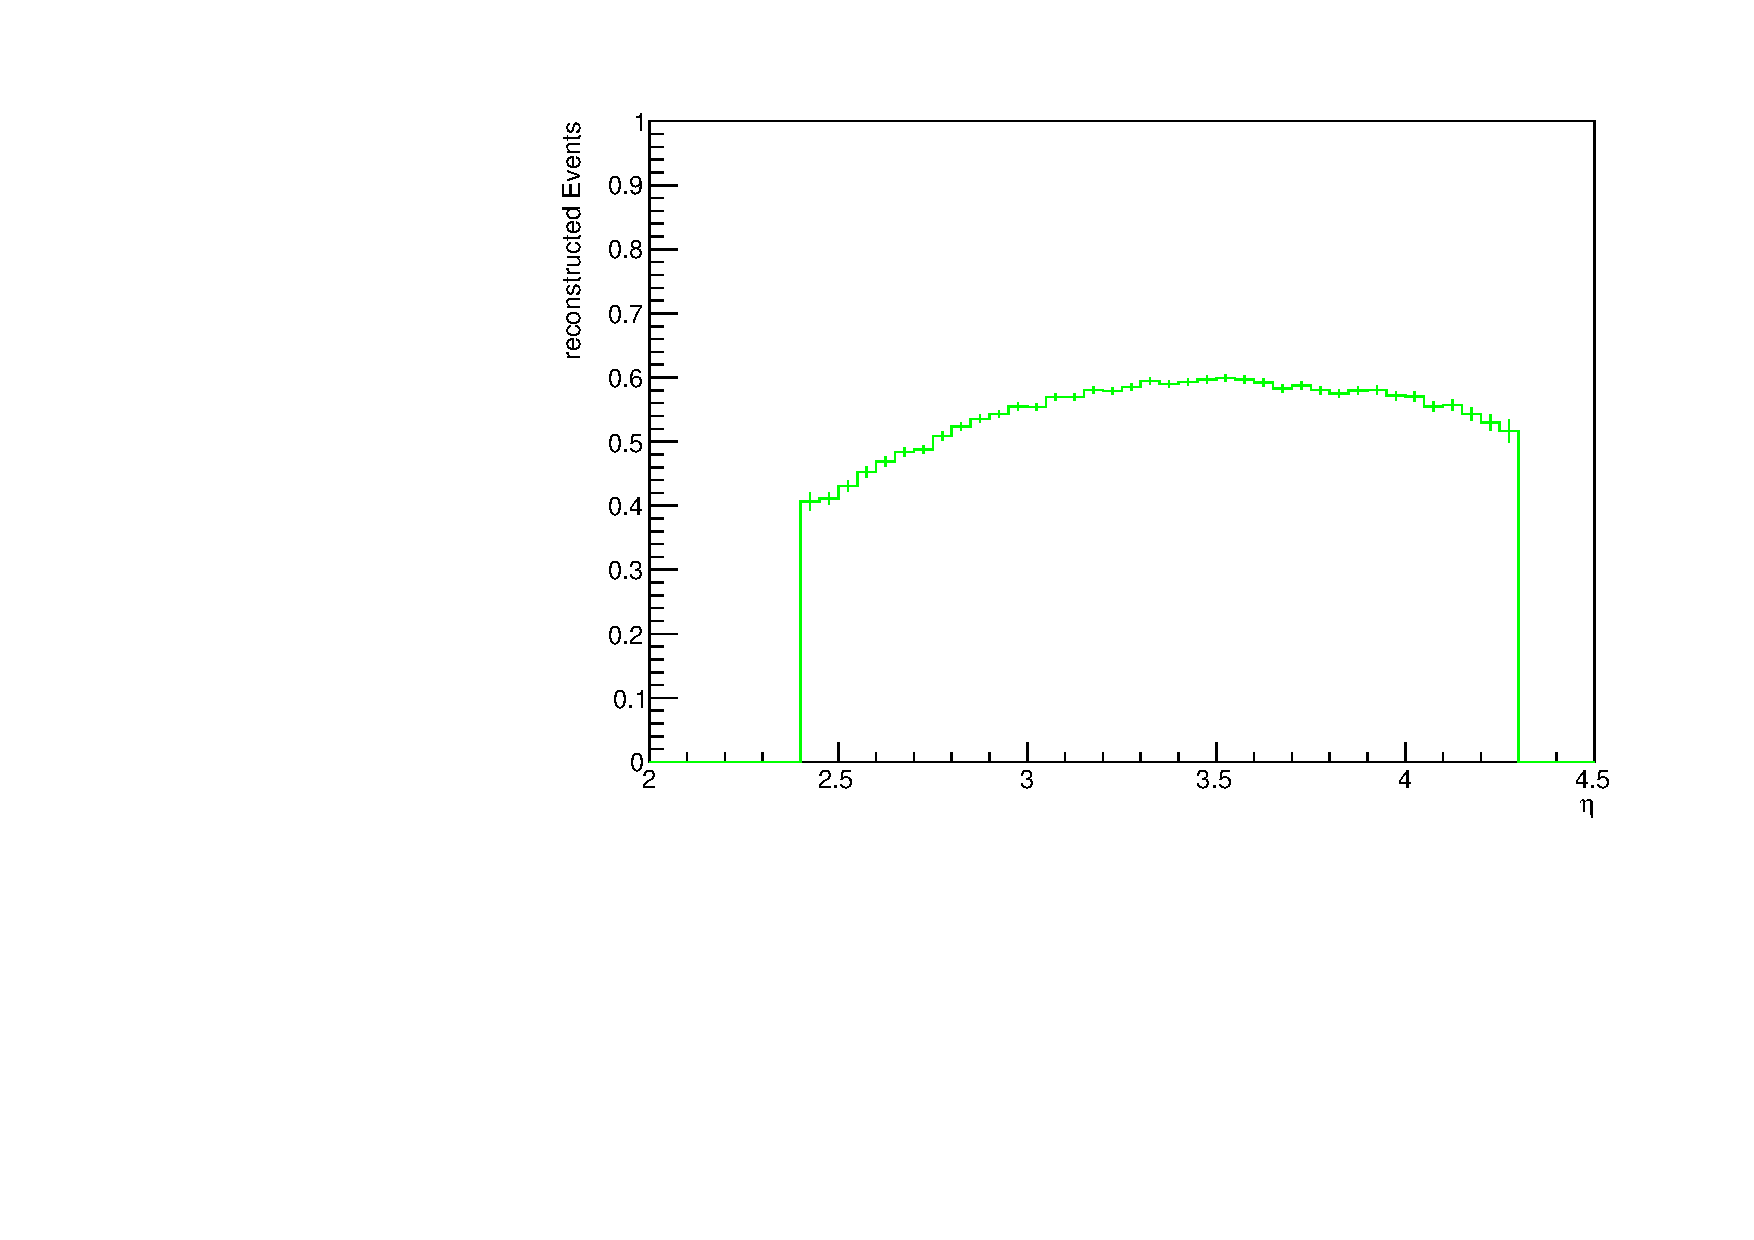
\includegraphics[width=0.9\textwidth]{up_pdf/single/tot/h_eta_reco_Dst.pdf}
\end{subfigure}
\end{figure}
\end{frame}
\begin{frame}{$D^0$-efficiency}
\begin{figure}
\begin{subfigure}{0.45\textwidth}
\includegraphics[width=0.9\textwidth]{up_pdf/single/tot/h_pt_reco_D0.pdf}
\end{subfigure}
\begin{subfigure}{0.45\textwidth}
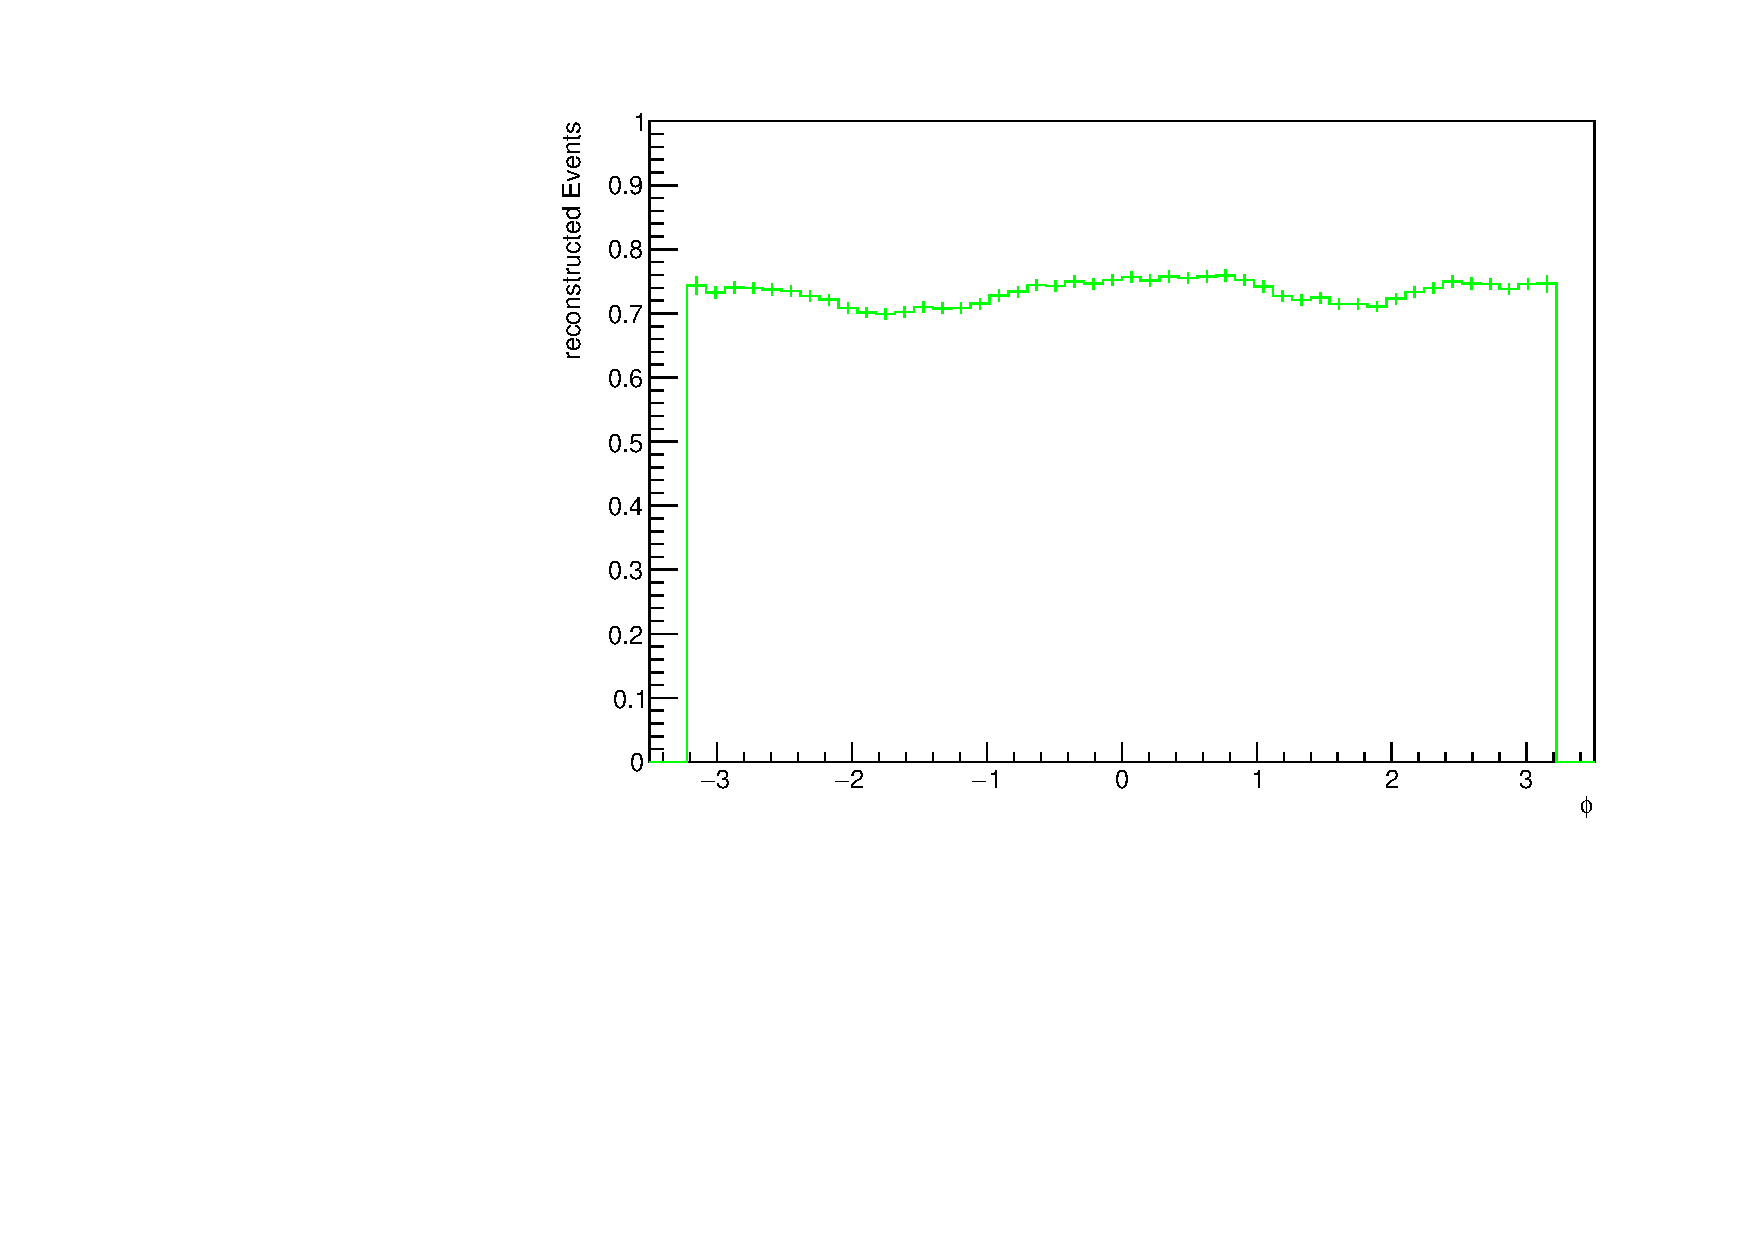
\includegraphics[width=0.9\textwidth]{up_pdf/single/tot/h_phi_reco_D0.pdf}
\end{subfigure}
\begin{subfigure}{0.45\textwidth}
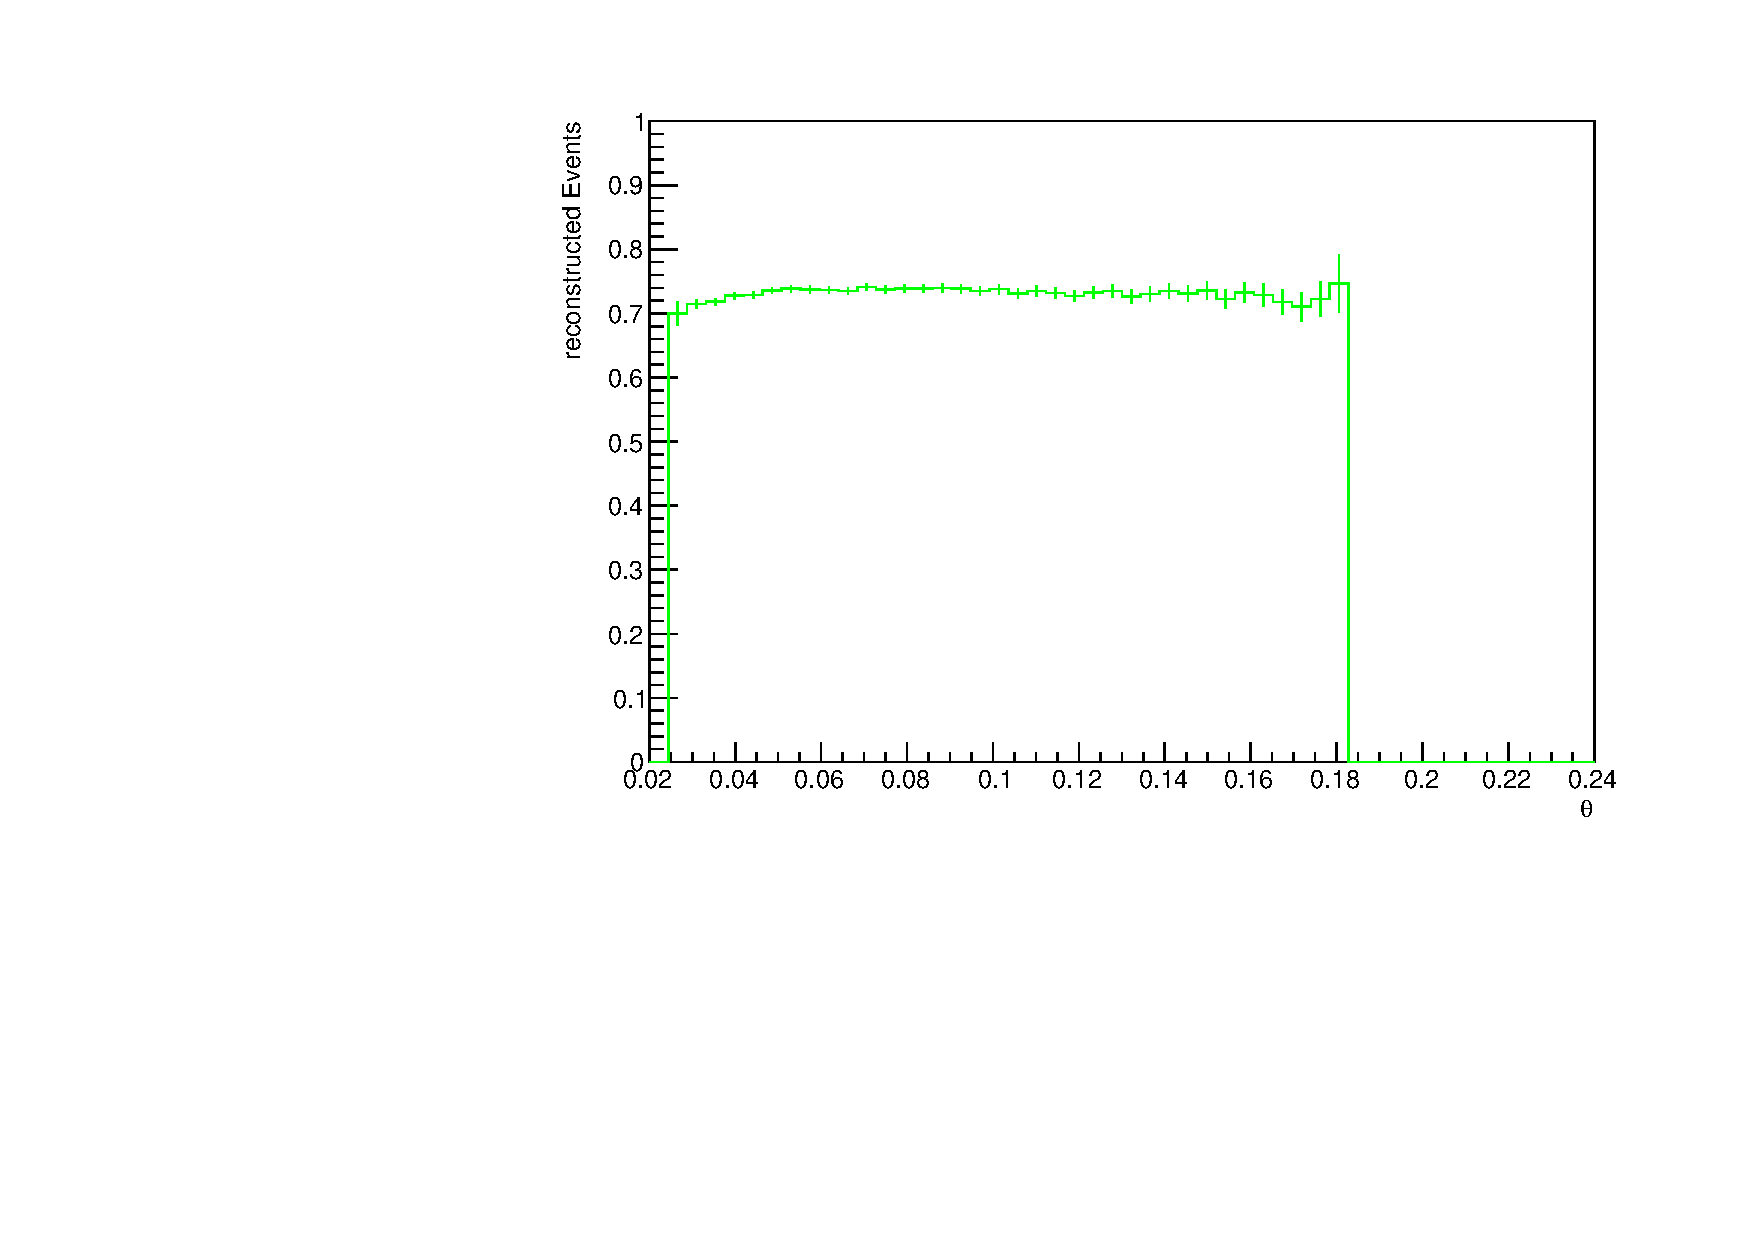
\includegraphics[width=0.9\textwidth]{up_pdf/single/tot/h_theta_reco_D0.pdf}
\end{subfigure}
\begin{subfigure}{0.45\textwidth}
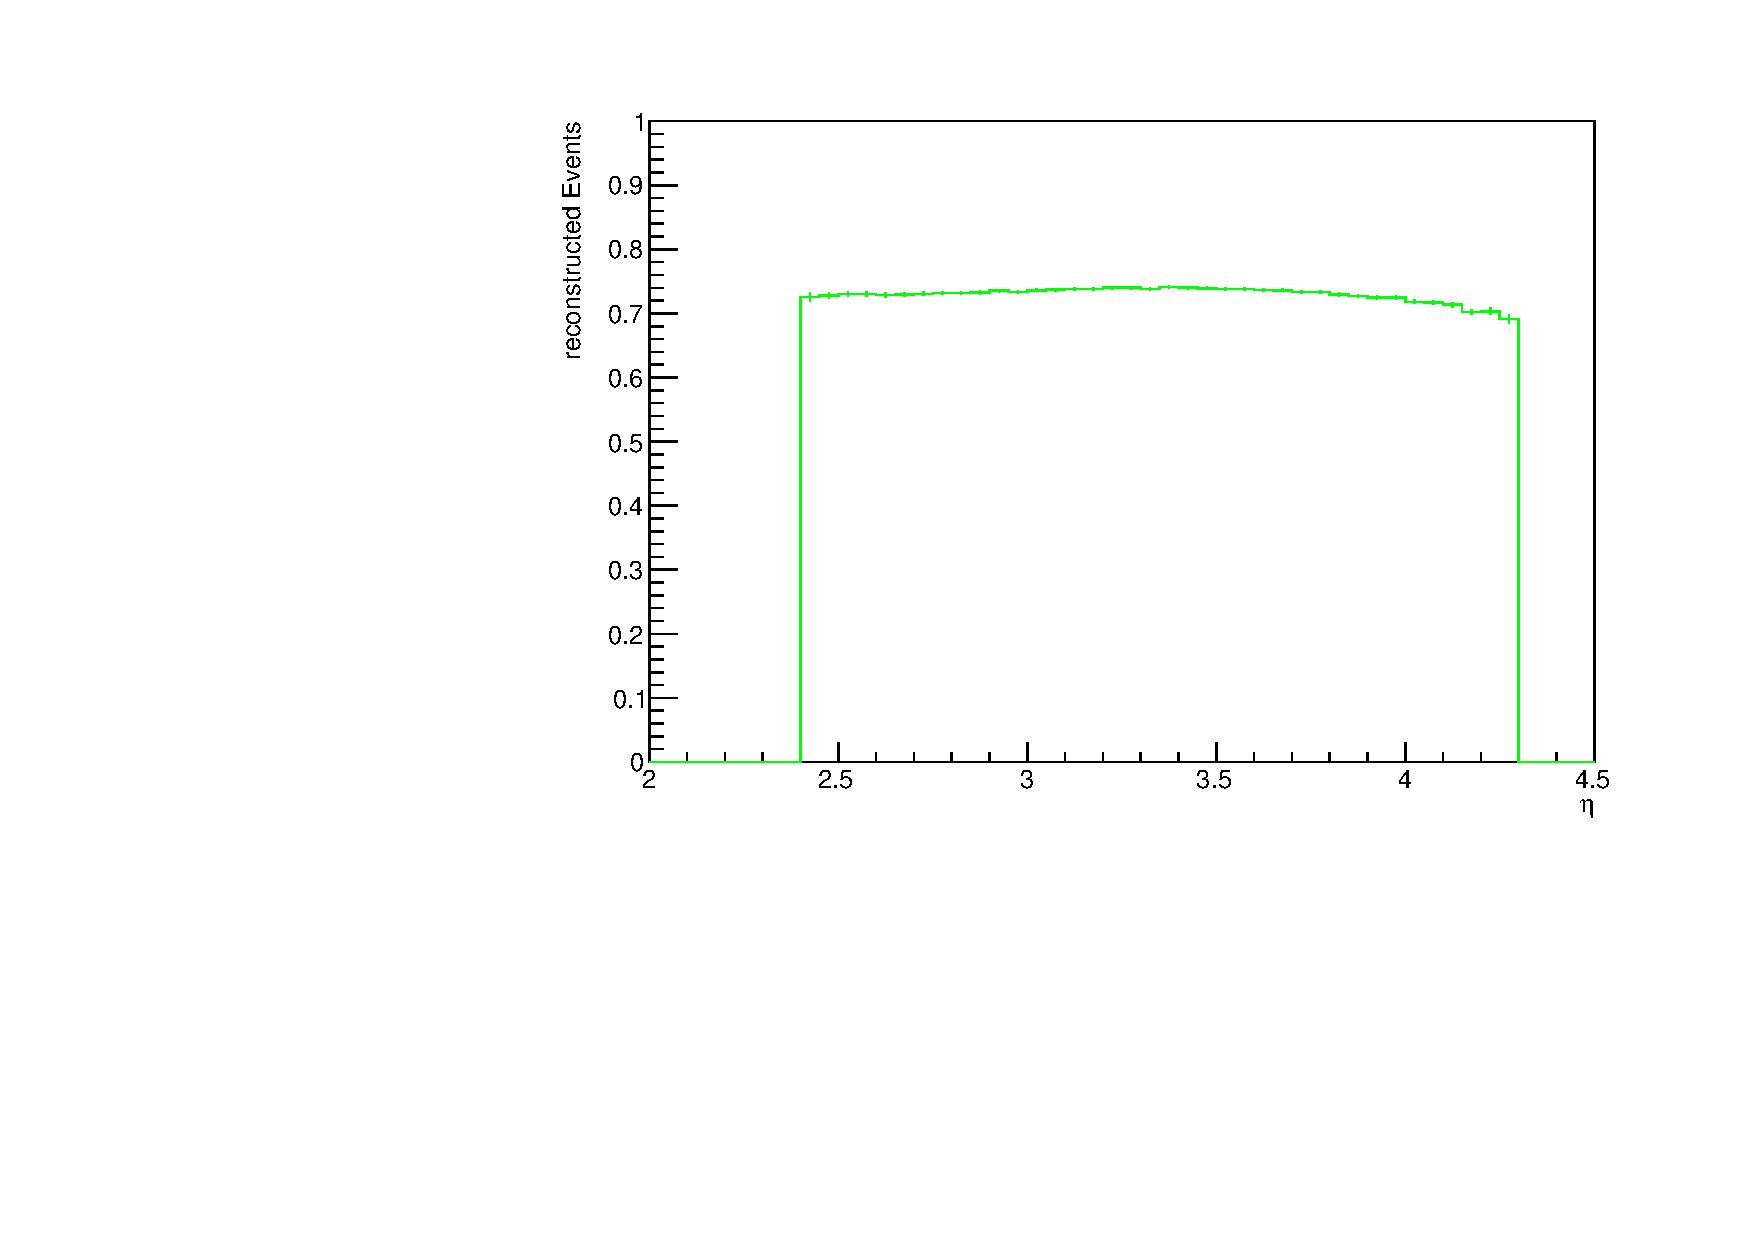
\includegraphics[width=0.9\textwidth]{up_pdf/single/tot/h_eta_reco_D0.pdf}
\end{subfigure}
\end{figure}
\end{frame}
\begin{frame}{$D^*$-efficiency}
\begin{figure}
\begin{subfigure}{0.45\textwidth}
\includegraphics[width=0.9\textwidth]{up_pdf/single/tot/h_pt_reco_Dst.pdf}
\end{subfigure}
\begin{subfigure}{0.45\textwidth}
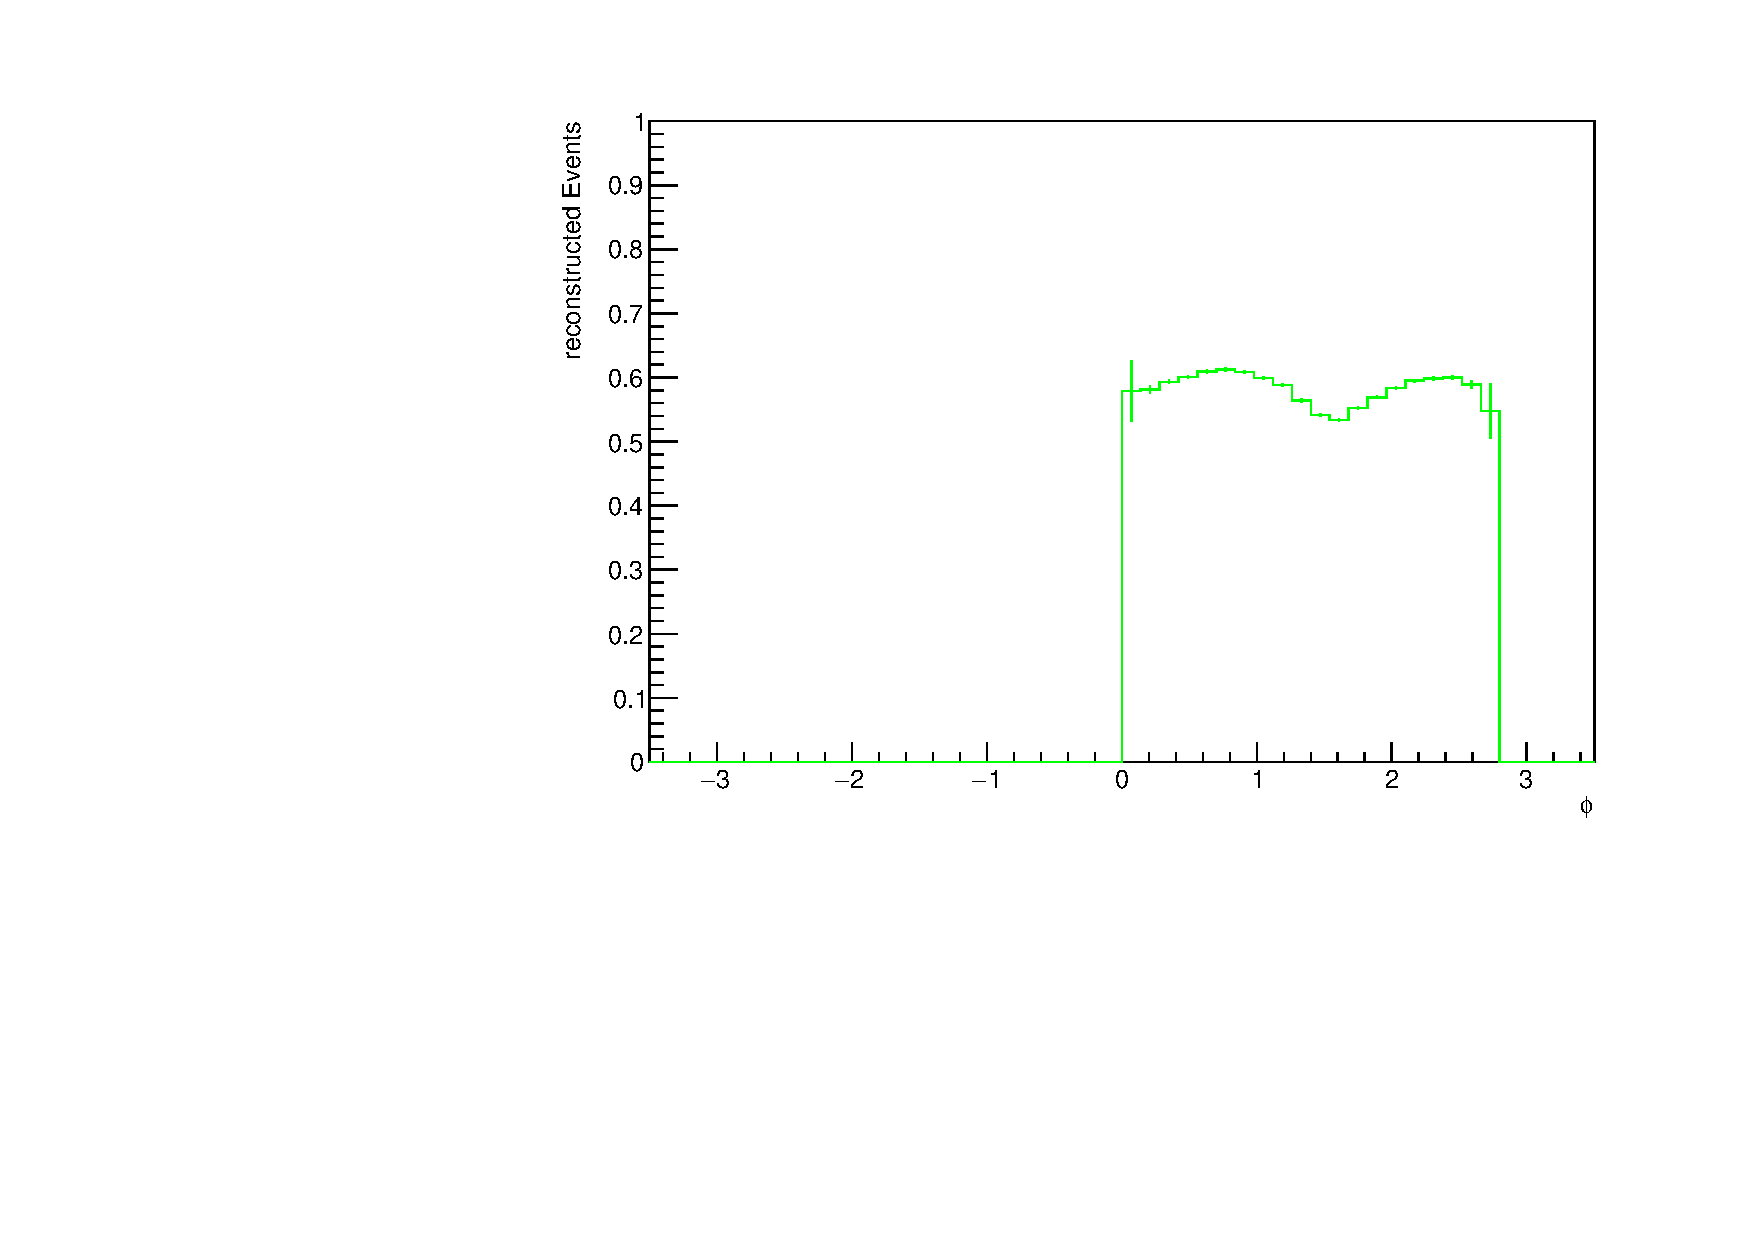
\includegraphics[width=0.9\textwidth]{up_pdf/single/tot/h_phi_reco_Dst.pdf}
\end{subfigure}
\begin{subfigure}{0.45\textwidth}
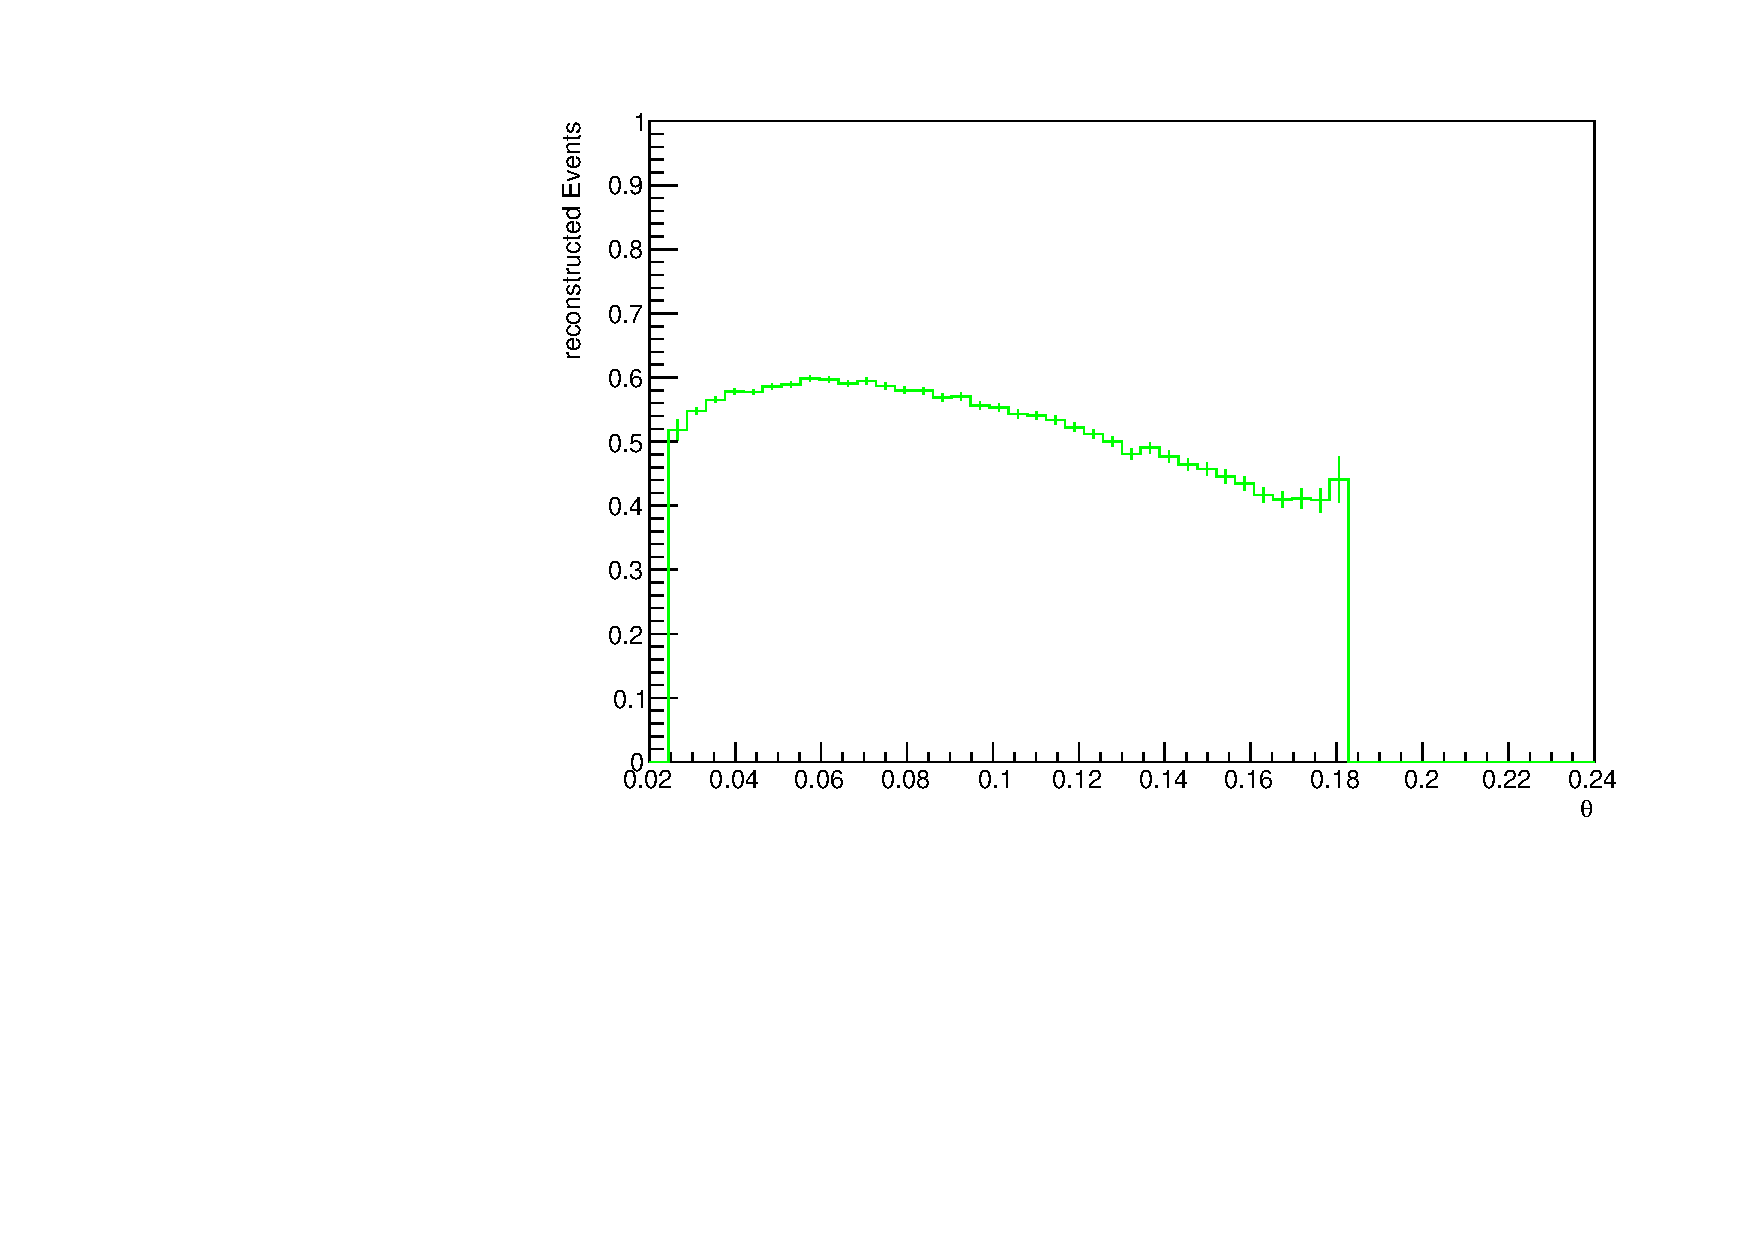
\includegraphics[width=0.9\textwidth]{up_pdf/single/tot/h_theta_reco_Dst.pdf}
\end{subfigure}
\begin{subfigure}{0.45\textwidth}
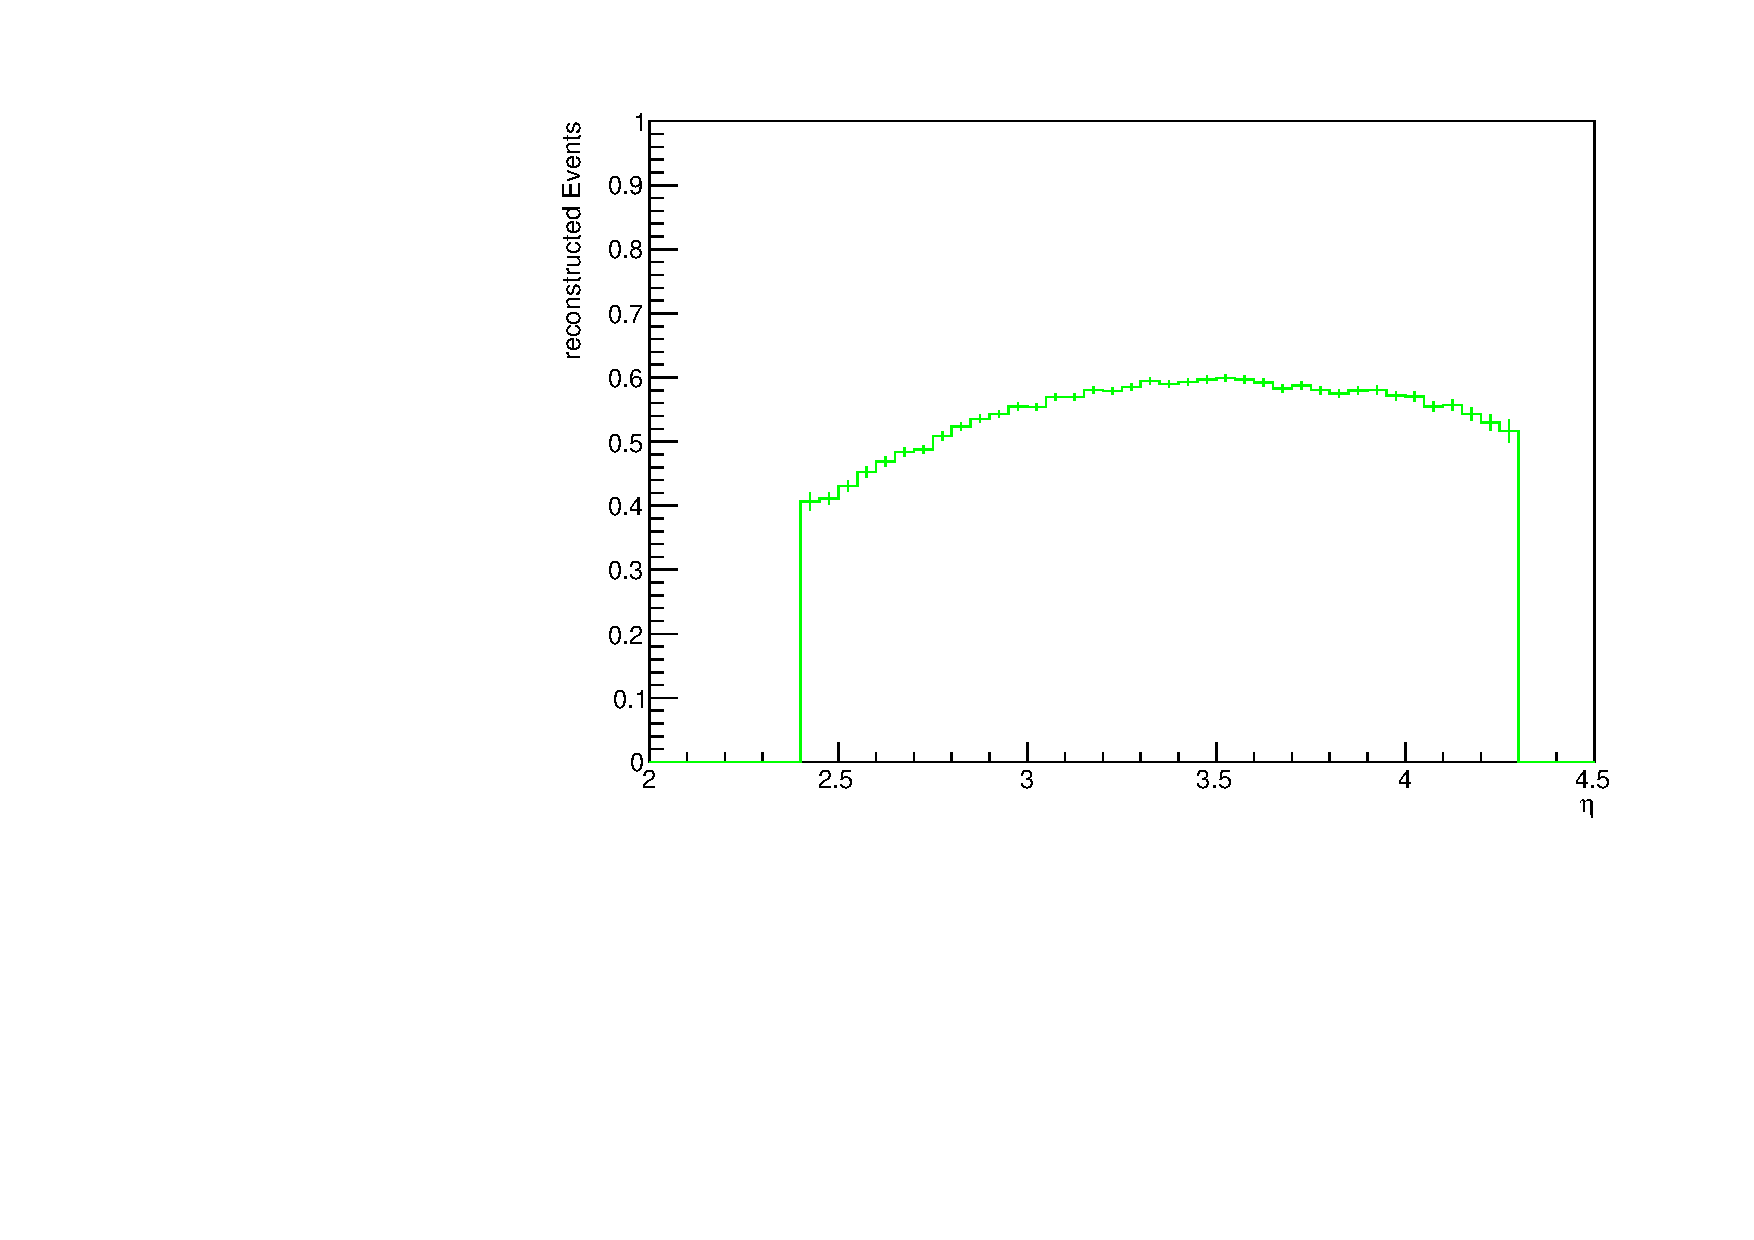
\includegraphics[width=0.9\textwidth]{up_pdf/single/tot/h_eta_reco_Dst.pdf}
\end{subfigure}
\end{figure}
\end{frame}
\begin{frame}
\begin{LARGE}
\textbf{Charge: +}
\end{LARGE}
\end{frame}
\begin{frame}{Efficiencies}
\begin{table}
\resizebox{\textwidth}{!}{
	\begin{tabular}{cS[table-format=2.2]@{${}\pm{}$}S[table-format=1.2]S[table-format=2.2]@{${}\pm{}$}S[table-format=1.2]S[table-format=2.2]@{${}\pm{}$}S[table-format=1.2]S[table-format=2.2]@{${}\pm{}$}S[table-format=1.2]S[table-format=2.2]@{${}\pm{}$}S[table-format=1.2]}
		\toprule
		{Polarity} & \multicolumn{2}{c}{$\epsilon_{\pi} $} & \multicolumn{2}{c}{$\epsilon_{K} $} & \multicolumn{2}{c}{$ \epsilon_{\pi,s} $} & \multicolumn{2}{c}{$\epsilon_{D^0} $} & \multicolumn{2}{c}{$\epsilon_{D^*} $} \\
		\midrule
		$UP$ & 86.63 & 0.06 & 85.01 & 0.06 & 76.26 & 0.07 & 73.00 & 0.07 & 55.71 & 0.08 \\
		$DOWN$ & 86.57 & 0.06 & 85.38 & 0.07 & 76.71 & 0.08 & 72.92 & 0.08 & 56.09 & 0.09\\
		\bottomrule
	\end{tabular}}
\end{table}
\end{frame}
\begin{frame}{$\pi$-efficiency}
\begin{figure}
\begin{subfigure}{0.45\textwidth}
\includegraphics[width=0.9\textwidth]{up_pdf/single/pos/h_pt_reco_Pi_pos.pdf}
\end{subfigure}
\begin{subfigure}{0.45\textwidth}
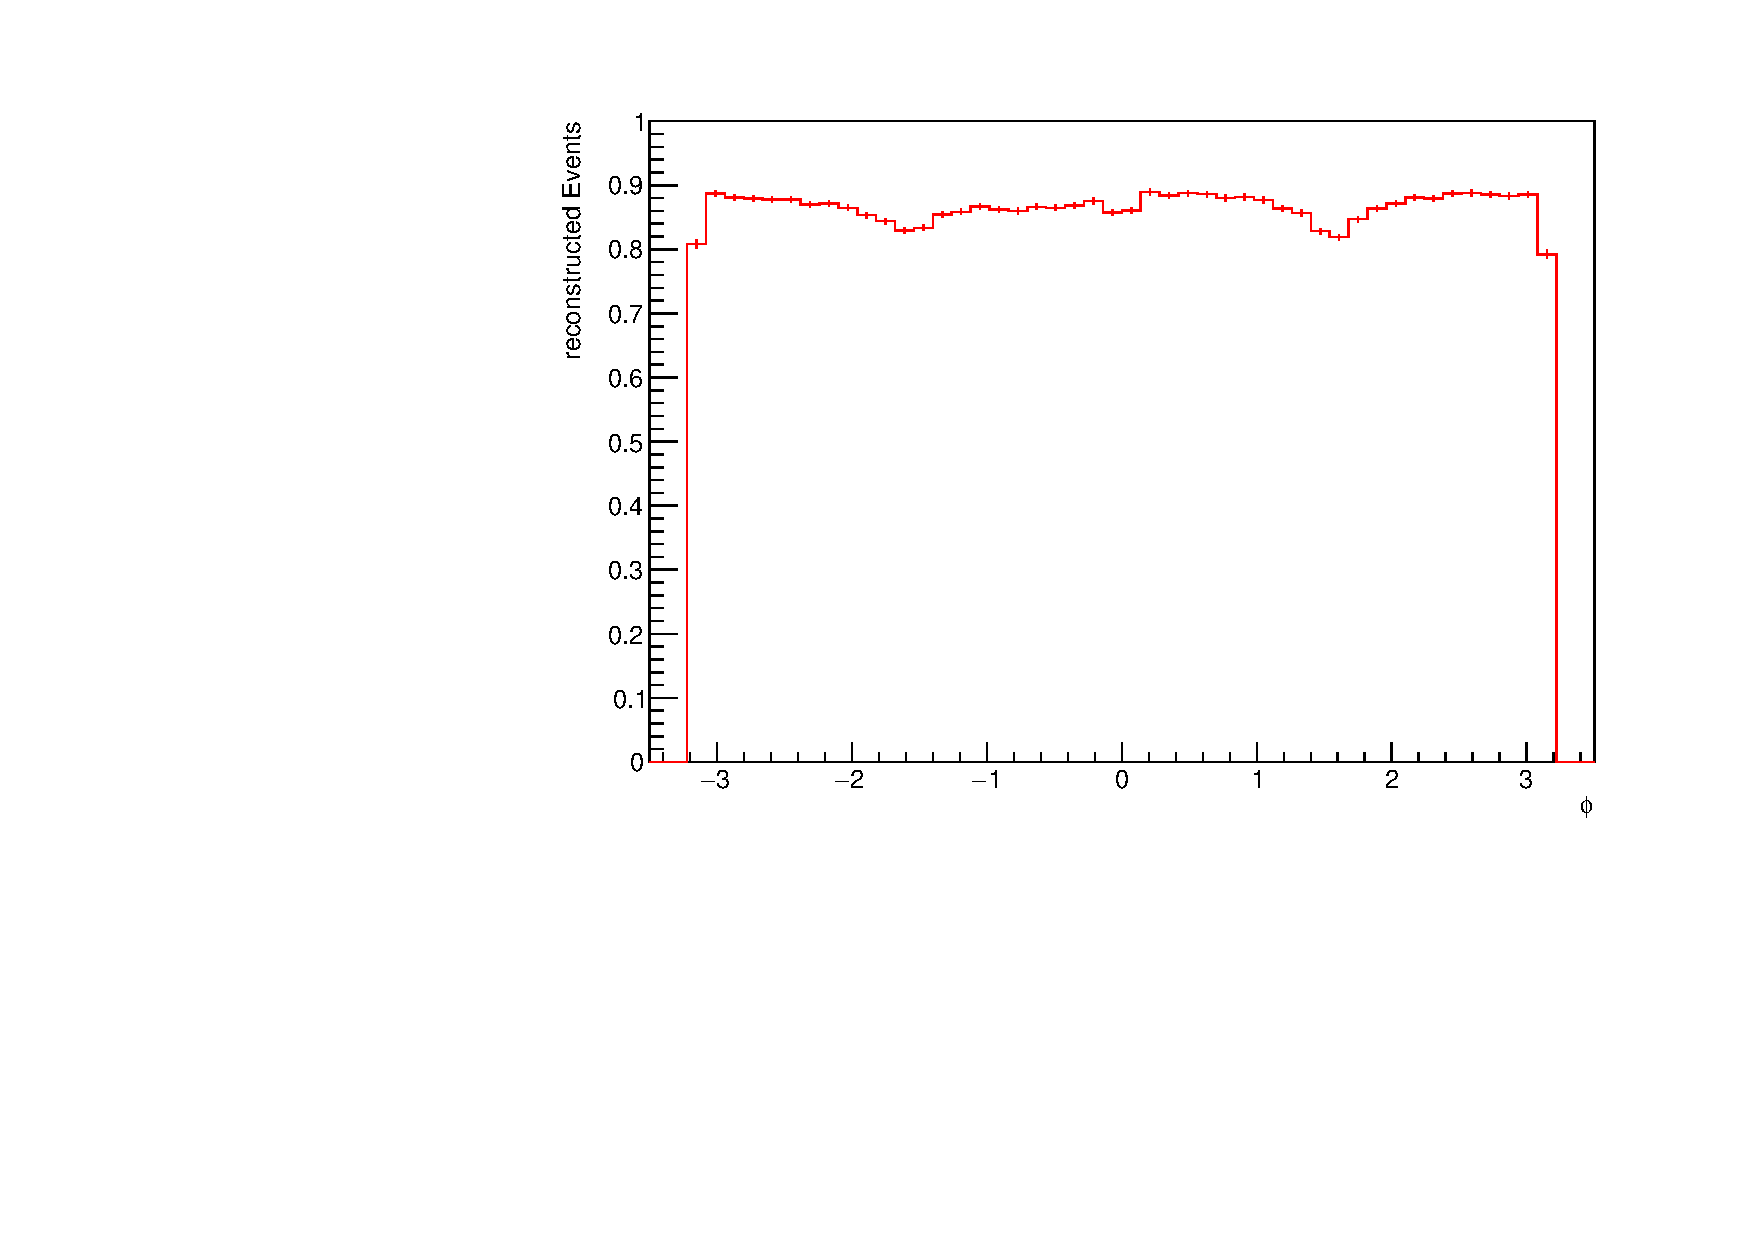
\includegraphics[width=0.9\textwidth]{up_pdf/single/pos/h_phi_reco_Pi_pos.pdf}
\end{subfigure}
\begin{subfigure}{0.45\textwidth}
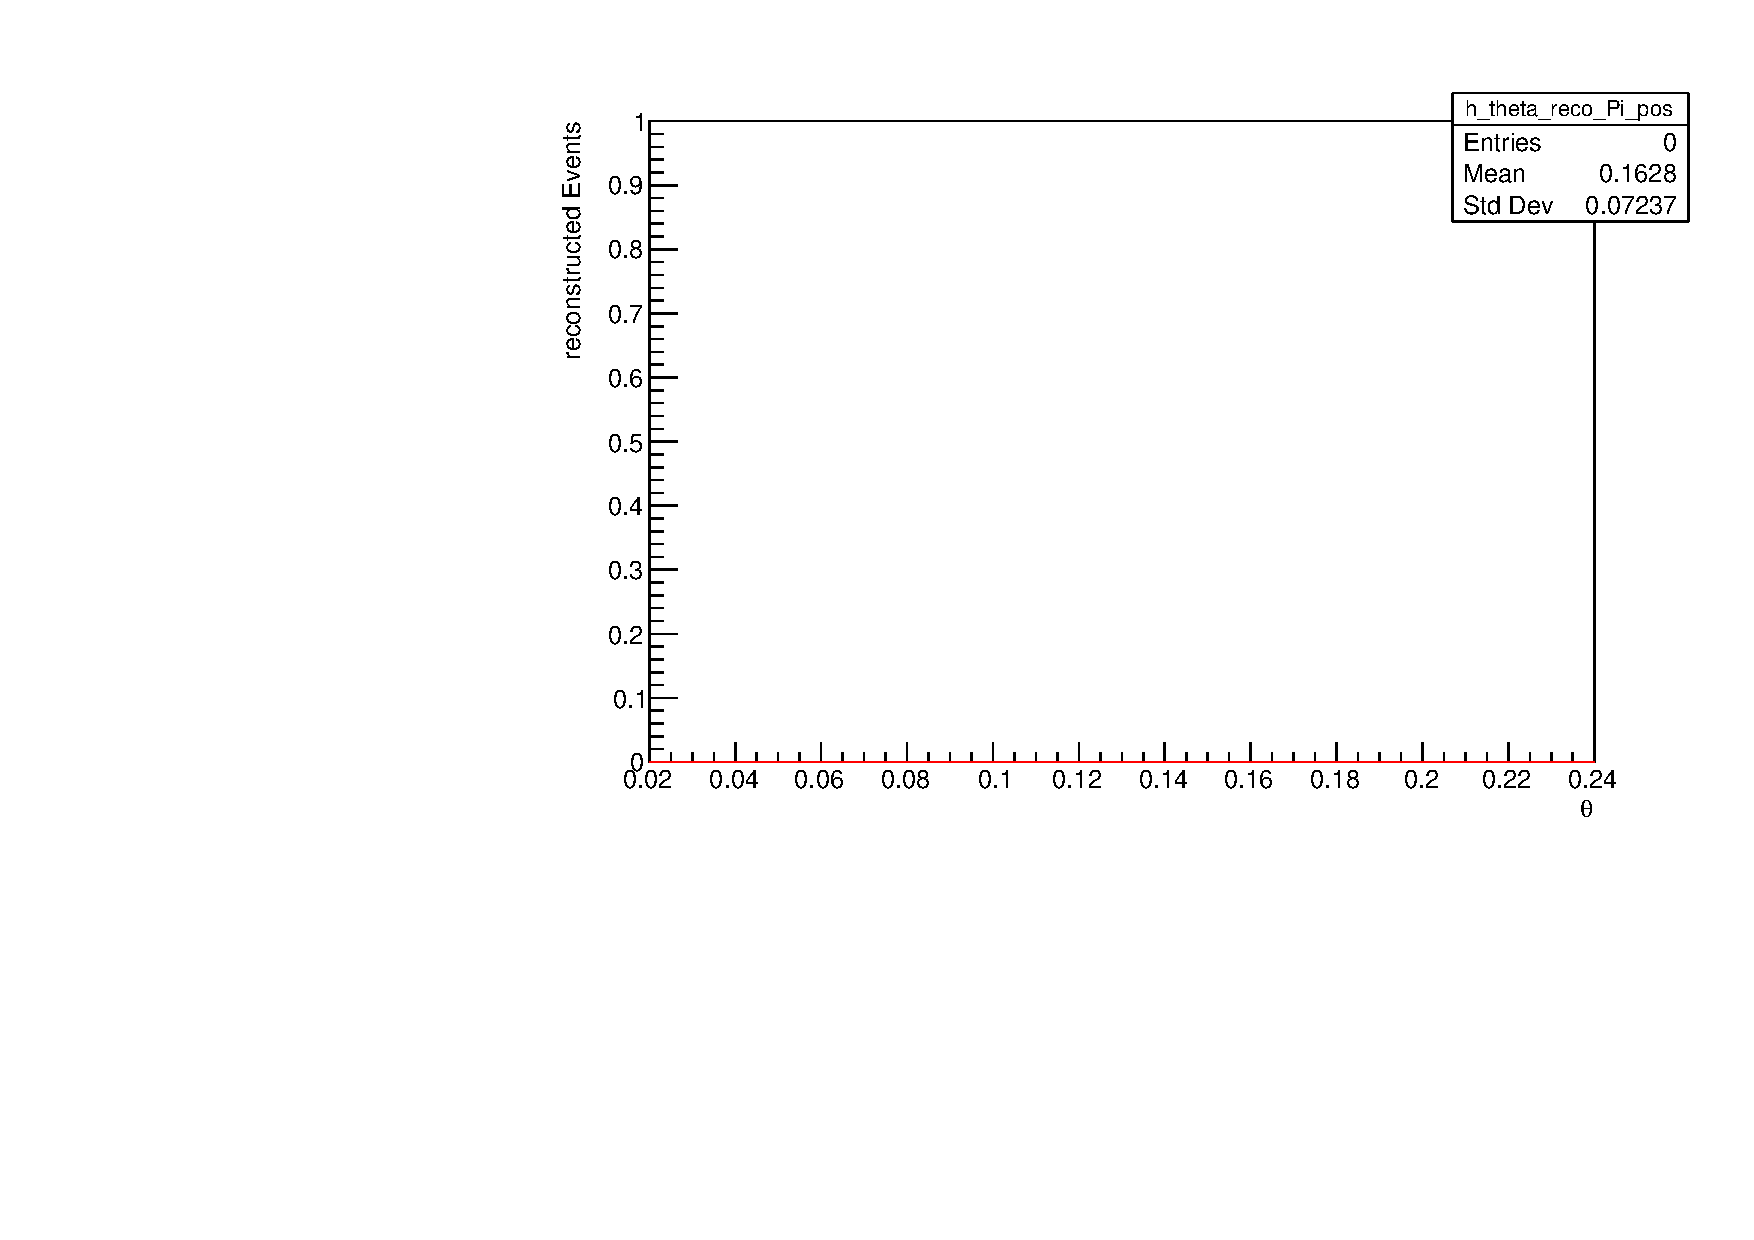
\includegraphics[width=0.9\textwidth]{up_pdf/single/pos/h_theta_reco_Pi_pos.pdf}
\end{subfigure}
\begin{subfigure}{0.45\textwidth}
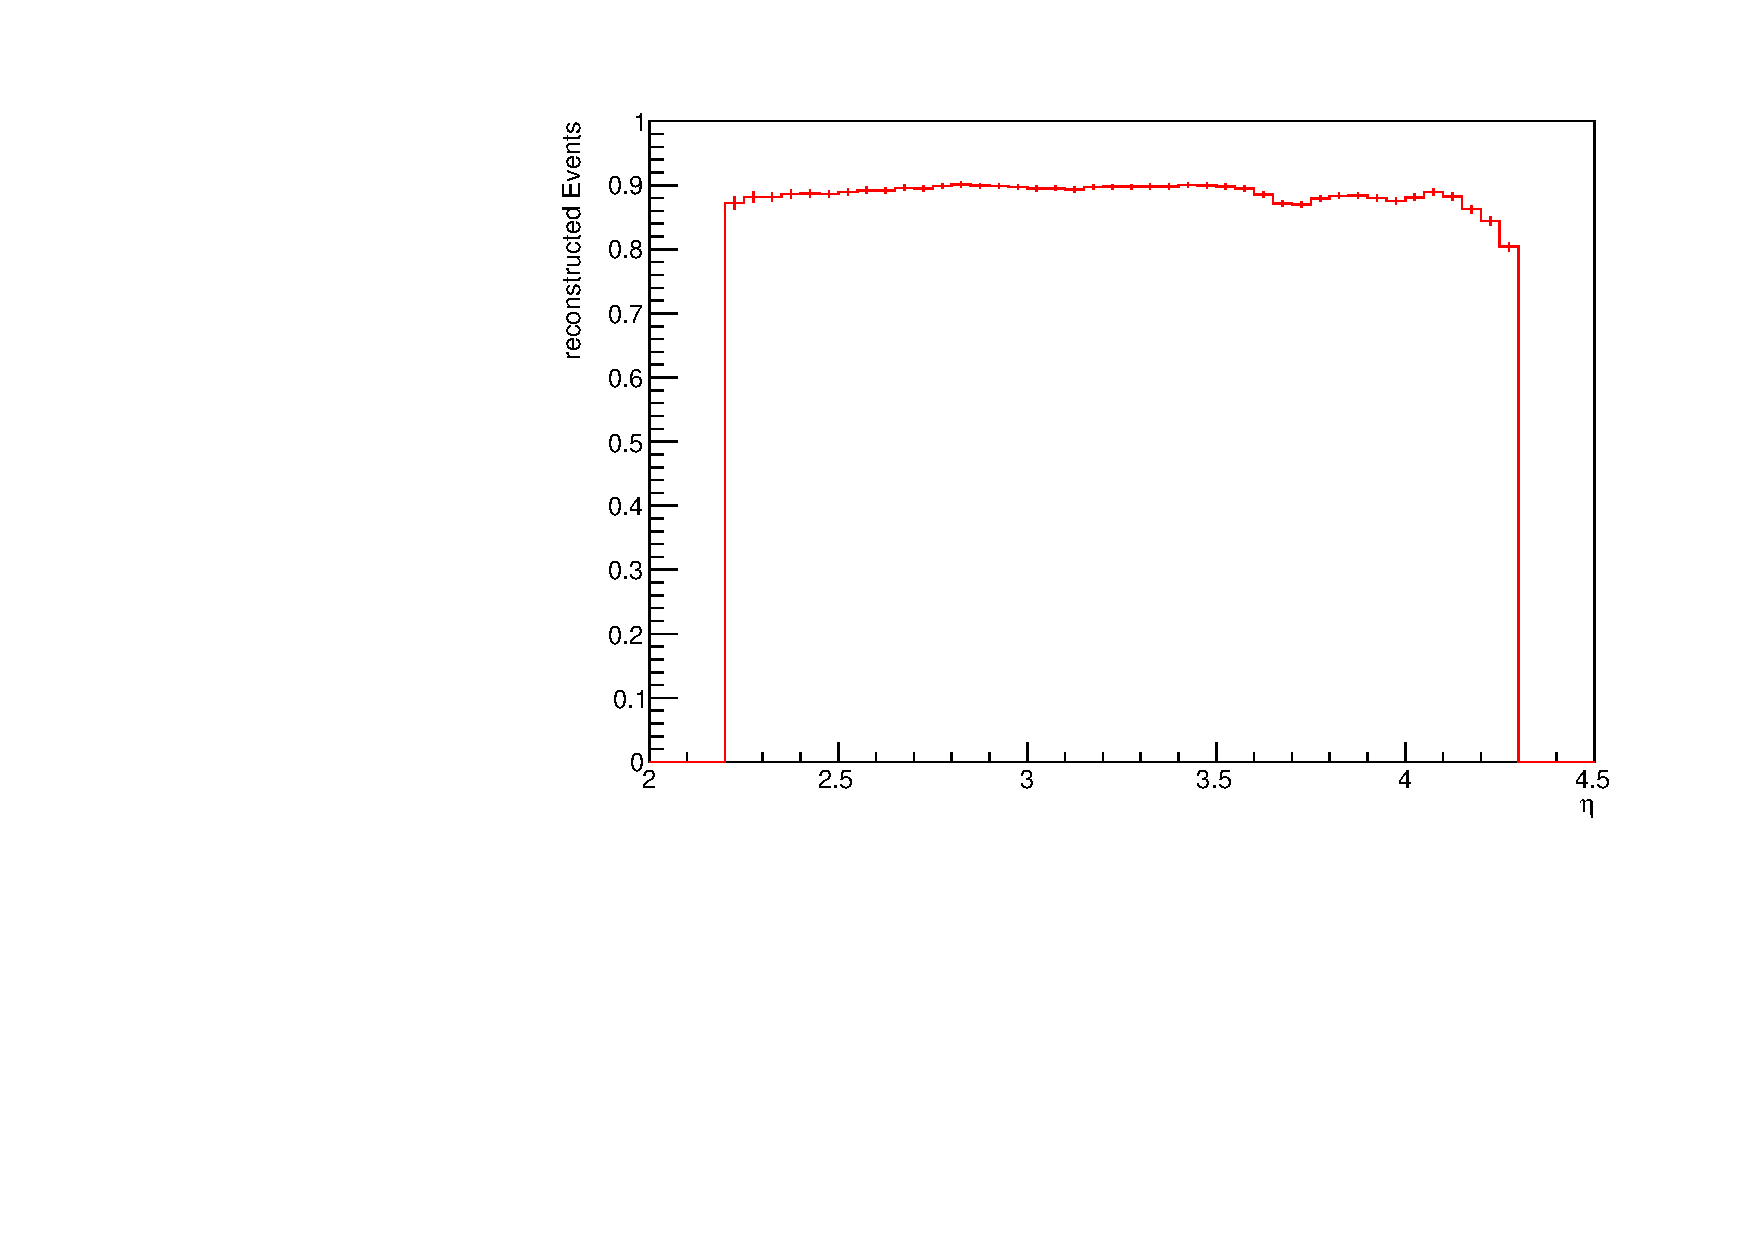
\includegraphics[width=0.9\textwidth]{up_pdf/single/pos/h_eta_reco_Pi_pos.pdf}
\end{subfigure}
\end{figure}
\end{frame}
\begin{frame}{$K$-efficiency}
\begin{figure}
\begin{subfigure}{0.45\textwidth}
\includegraphics[width=0.9\textwidth]{up_pdf/single/pos/h_pt_reco_K_pos.pdf}
\end{subfigure}
\begin{subfigure}{0.45\textwidth}
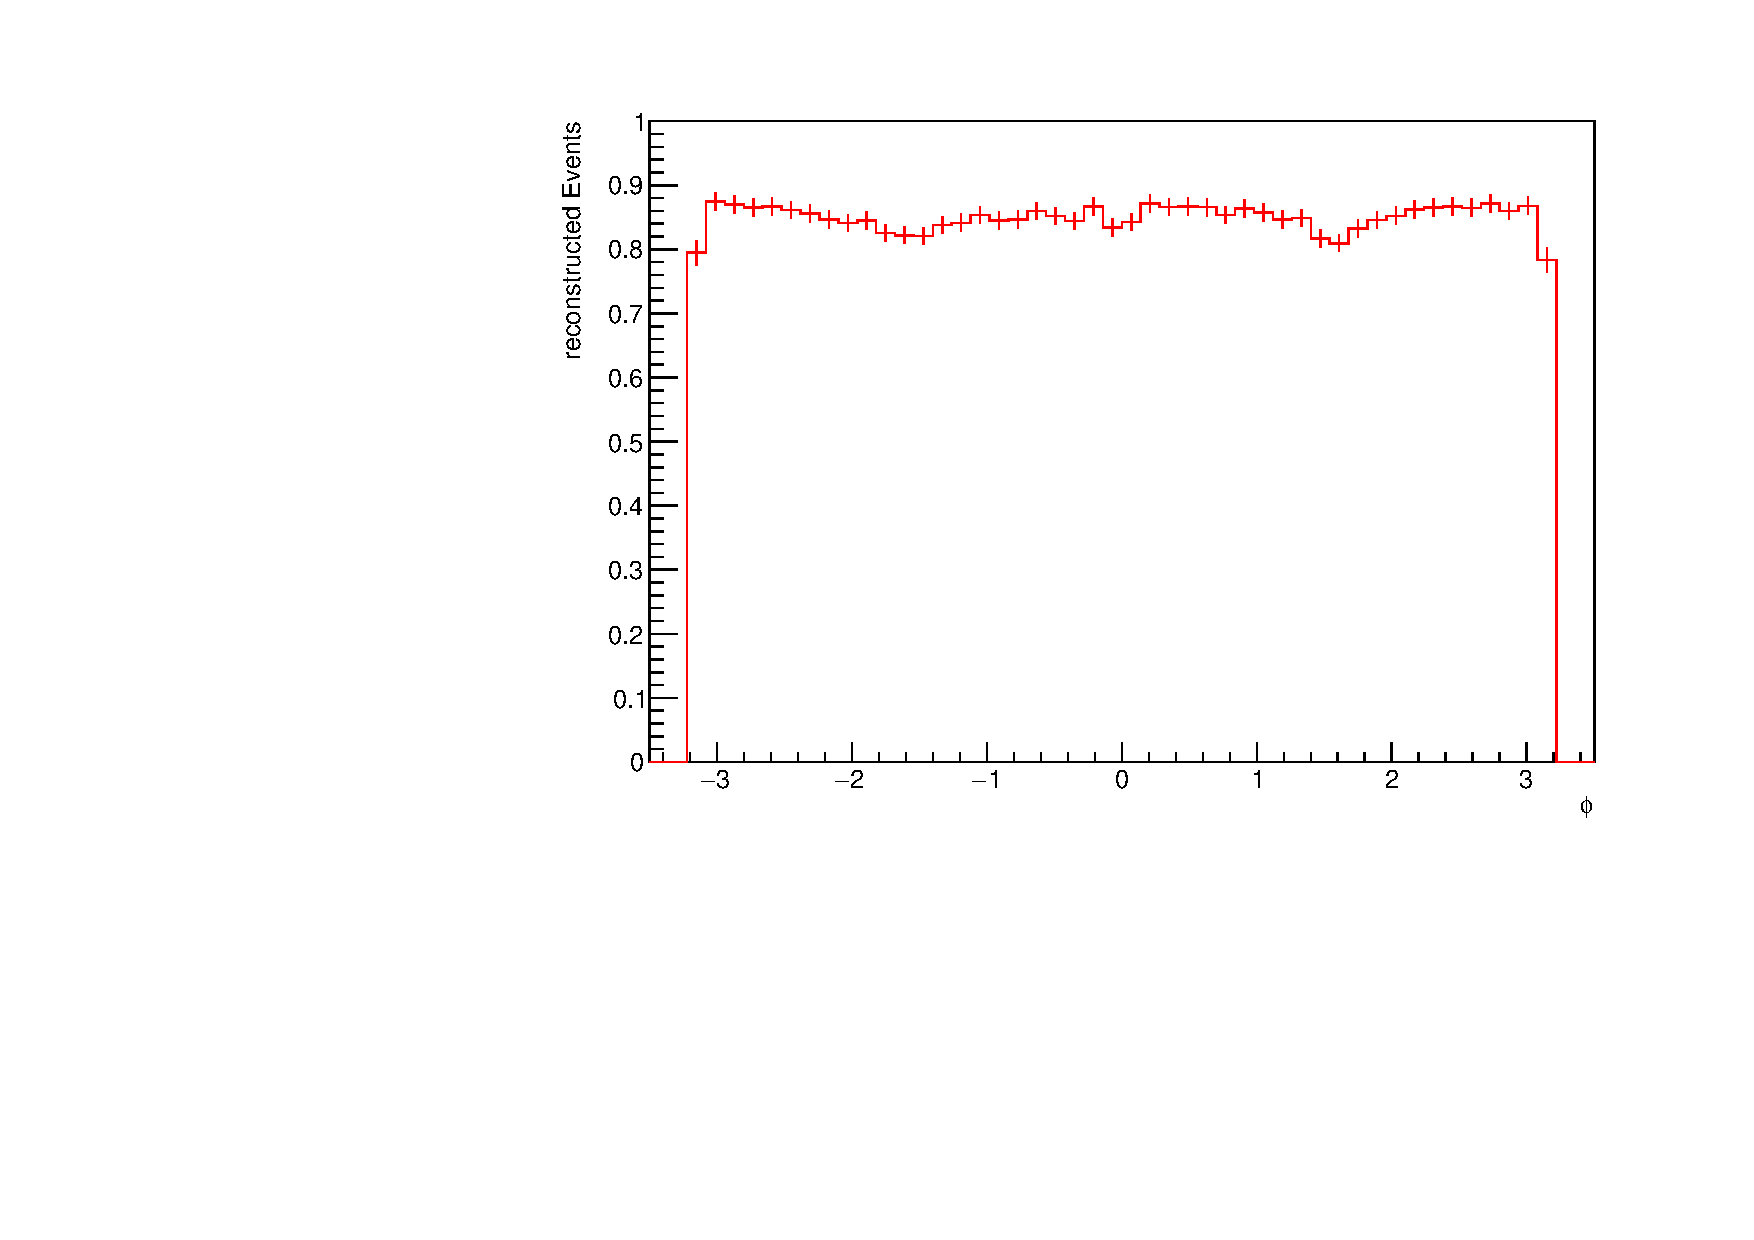
\includegraphics[width=0.9\textwidth]{up_pdf/single/pos/h_phi_reco_K_pos.pdf}
\end{subfigure}
\begin{subfigure}{0.45\textwidth}
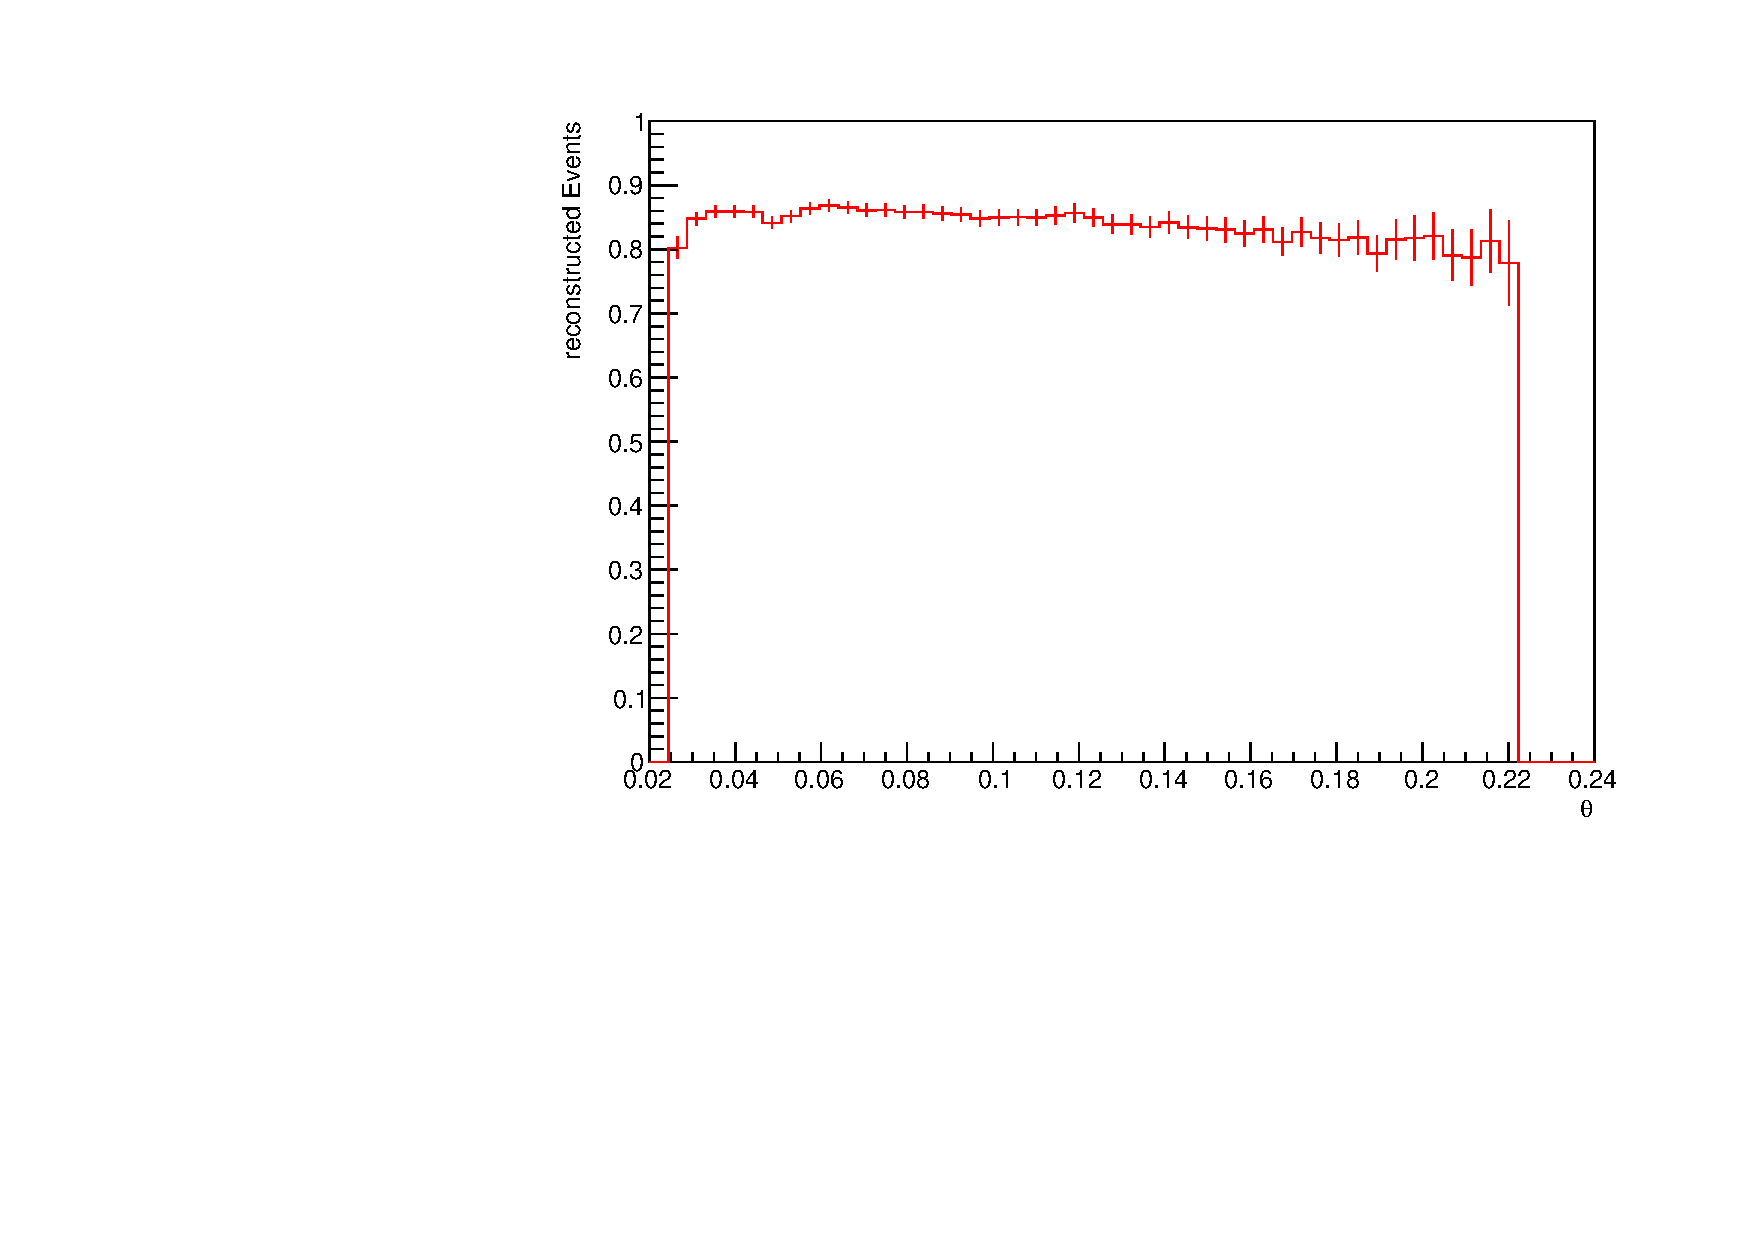
\includegraphics[width=0.9\textwidth]{up_pdf/single/pos/h_theta_reco_K_pos.pdf}
\end{subfigure}
\begin{subfigure}{0.45\textwidth}
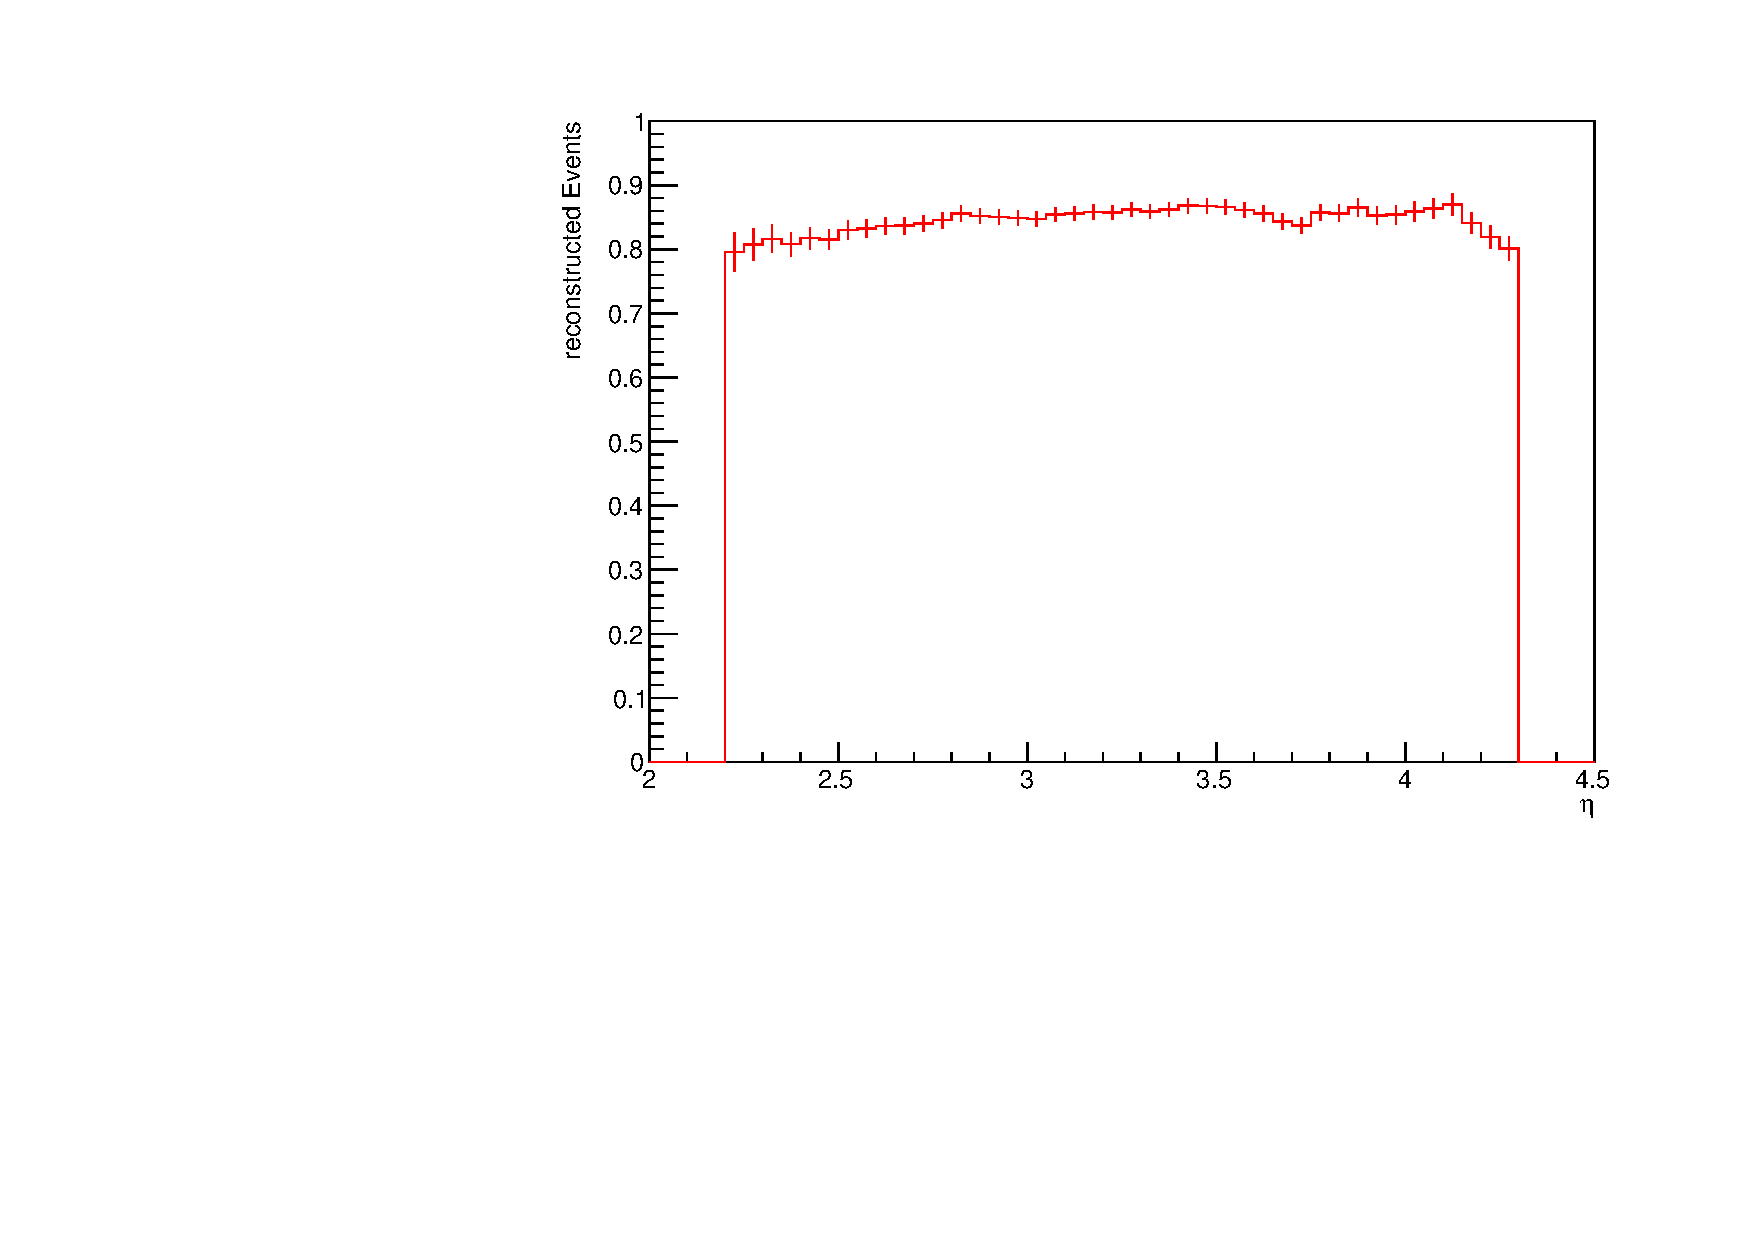
\includegraphics[width=0.9\textwidth]{up_pdf/single/pos/h_eta_reco_K_pos.pdf}
\end{subfigure}
\end{figure}
\end{frame}
\begin{frame}{soft $\pi$-efficiency}
\begin{figure}
\begin{subfigure}{0.45\textwidth}
\includegraphics[width=0.9\textwidth]{up_pdf/single/pos/h_pt_reco_SPi_pos.pdf}
\end{subfigure}
\begin{subfigure}{0.45\textwidth}
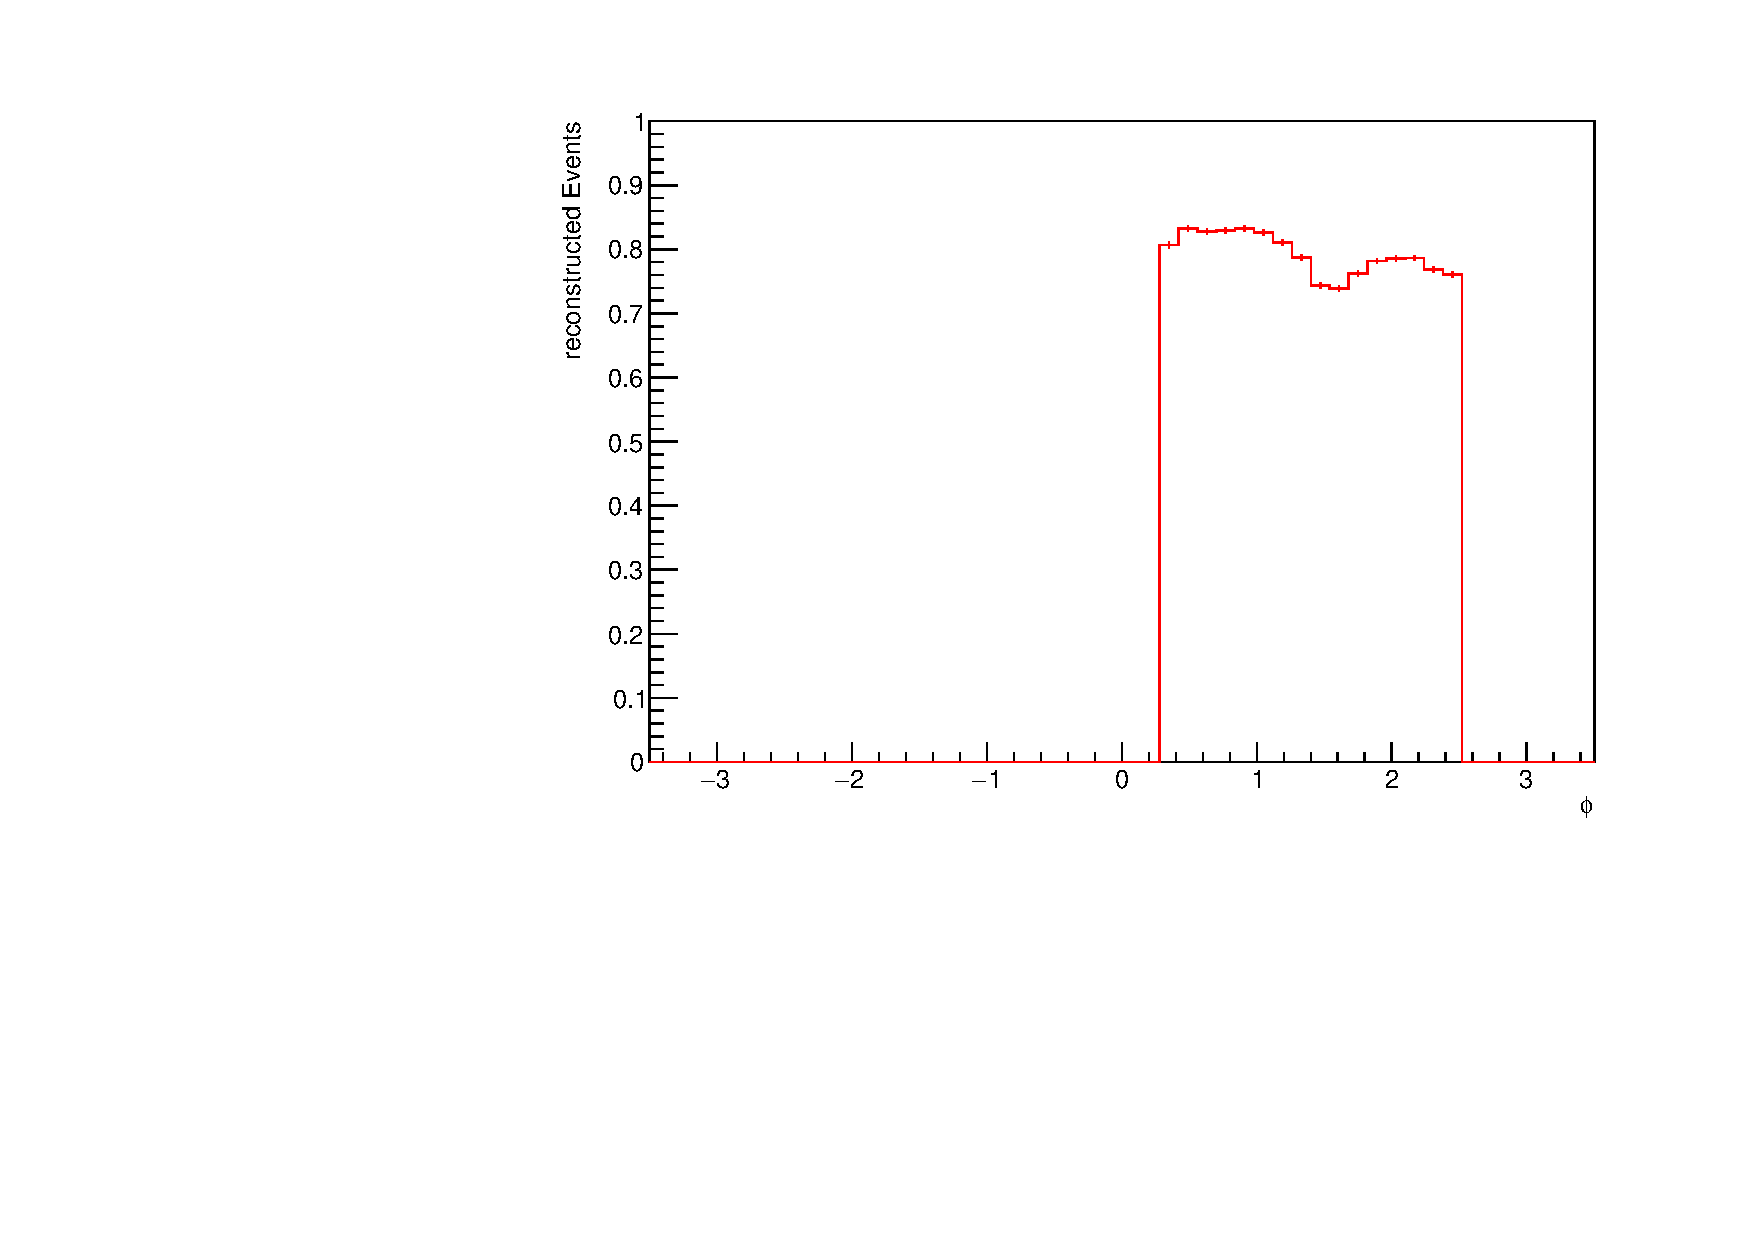
\includegraphics[width=0.9\textwidth]{up_pdf/single/pos/h_phi_reco_SPi_pos.pdf}
\end{subfigure}
\begin{subfigure}{0.45\textwidth}
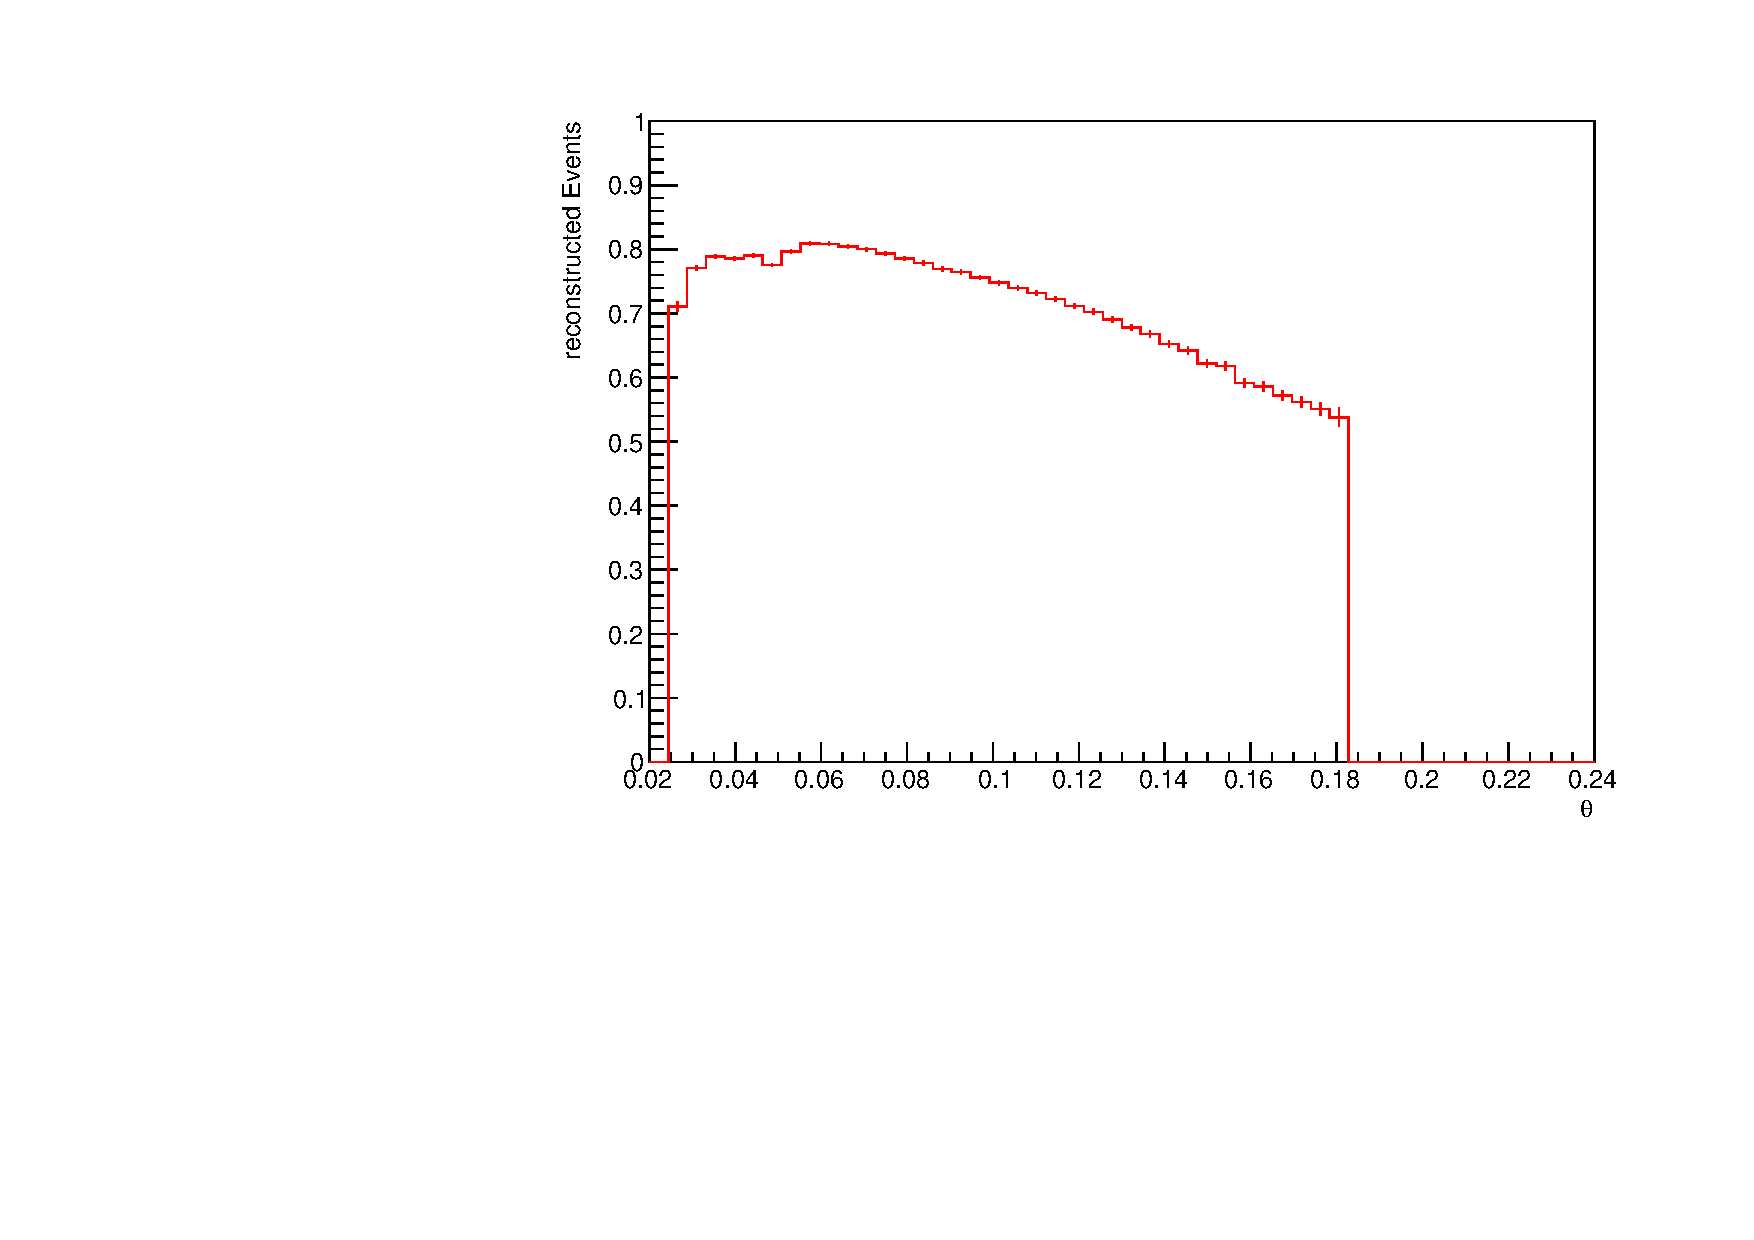
\includegraphics[width=0.9\textwidth]{up_pdf/single/pos/h_theta_reco_SPi_pos.pdf}
\end{subfigure}
\begin{subfigure}{0.45\textwidth}
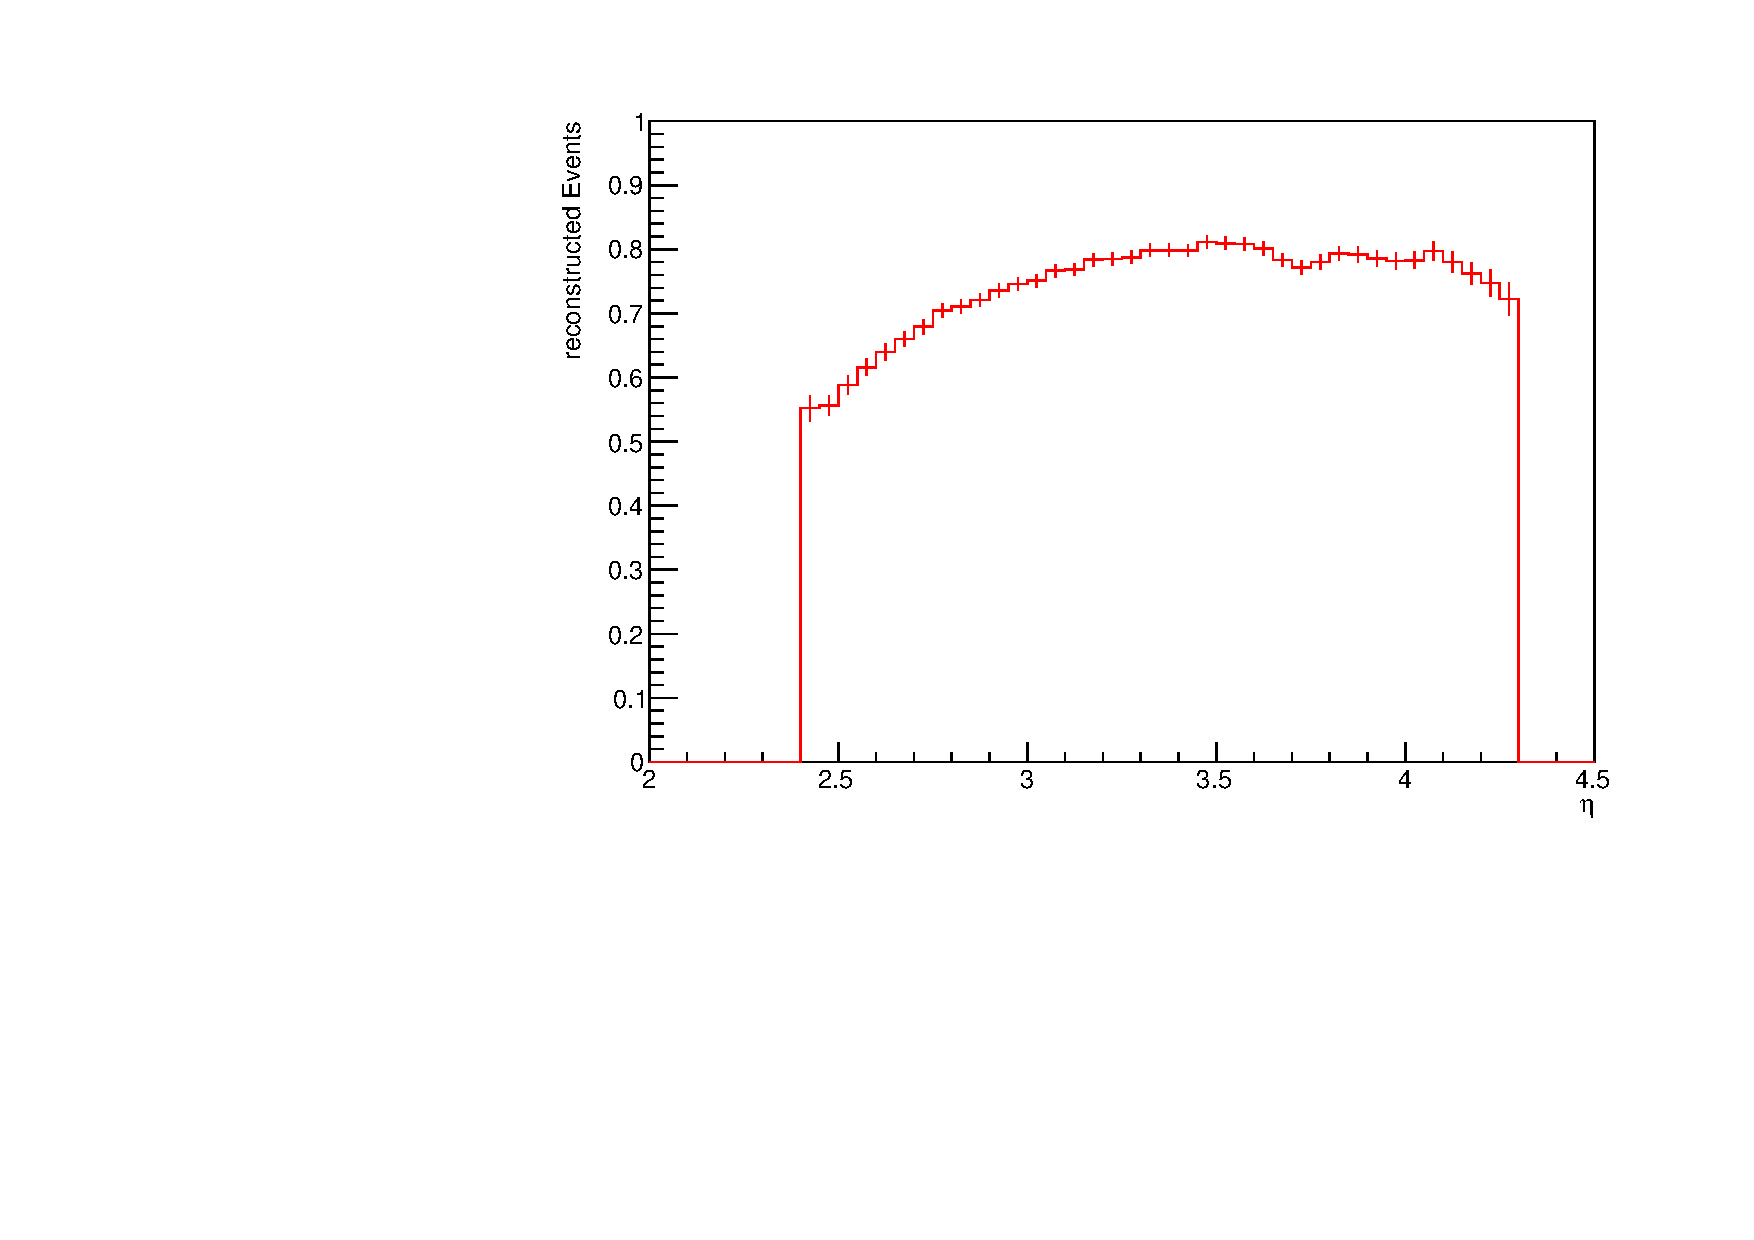
\includegraphics[width=0.9\textwidth]{up_pdf/single/pos/h_eta_reco_SPi_pos.pdf}
\end{subfigure}
\end{figure}
\end{frame}
\begin{frame}{$D^0$-efficiency}
\begin{figure}
\begin{subfigure}{0.45\textwidth}
\includegraphics[width=0.9\textwidth]{up_pdf/single/pos/h_pt_reco_D0_pos.pdf}
\end{subfigure}
\begin{subfigure}{0.45\textwidth}
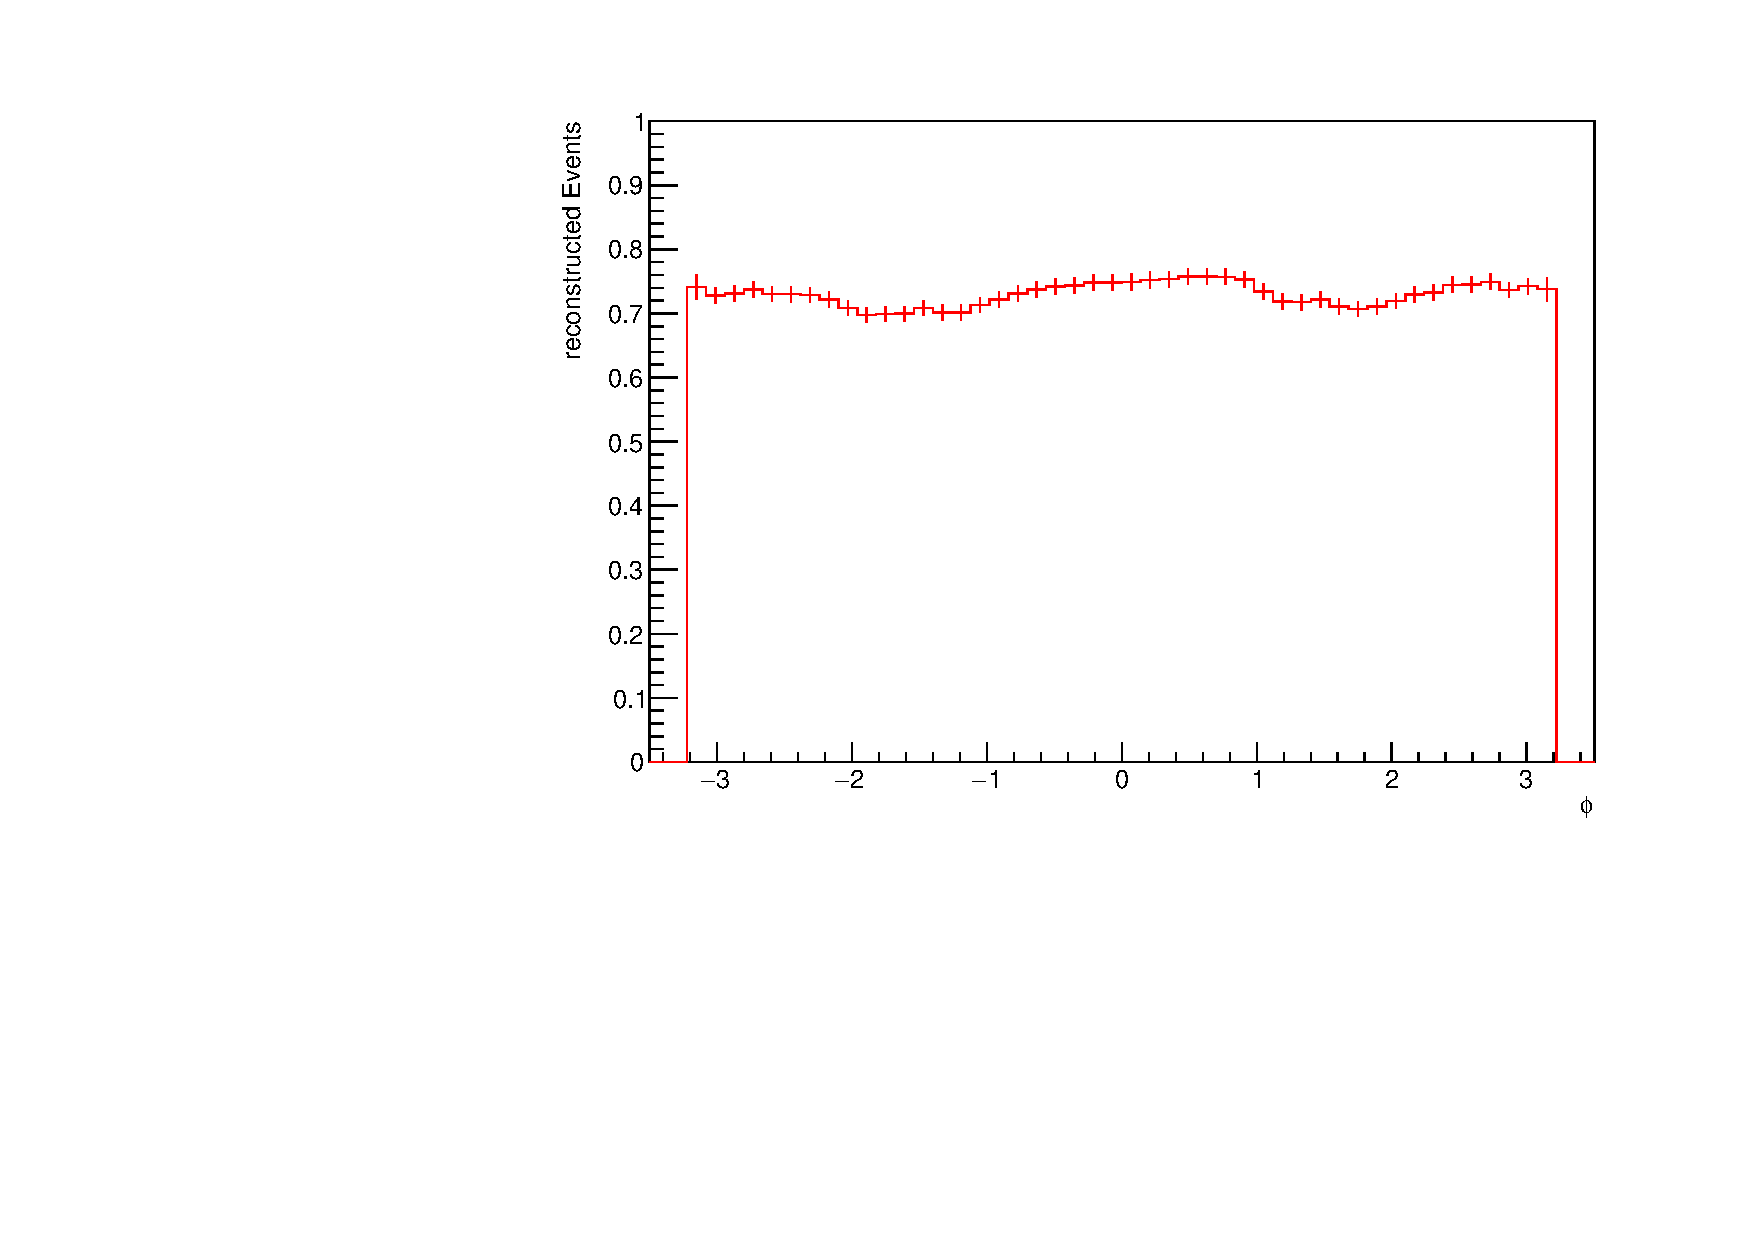
\includegraphics[width=0.9\textwidth]{up_pdf/single/pos/h_phi_reco_D0_pos.pdf}
\end{subfigure}
\begin{subfigure}{0.45\textwidth}
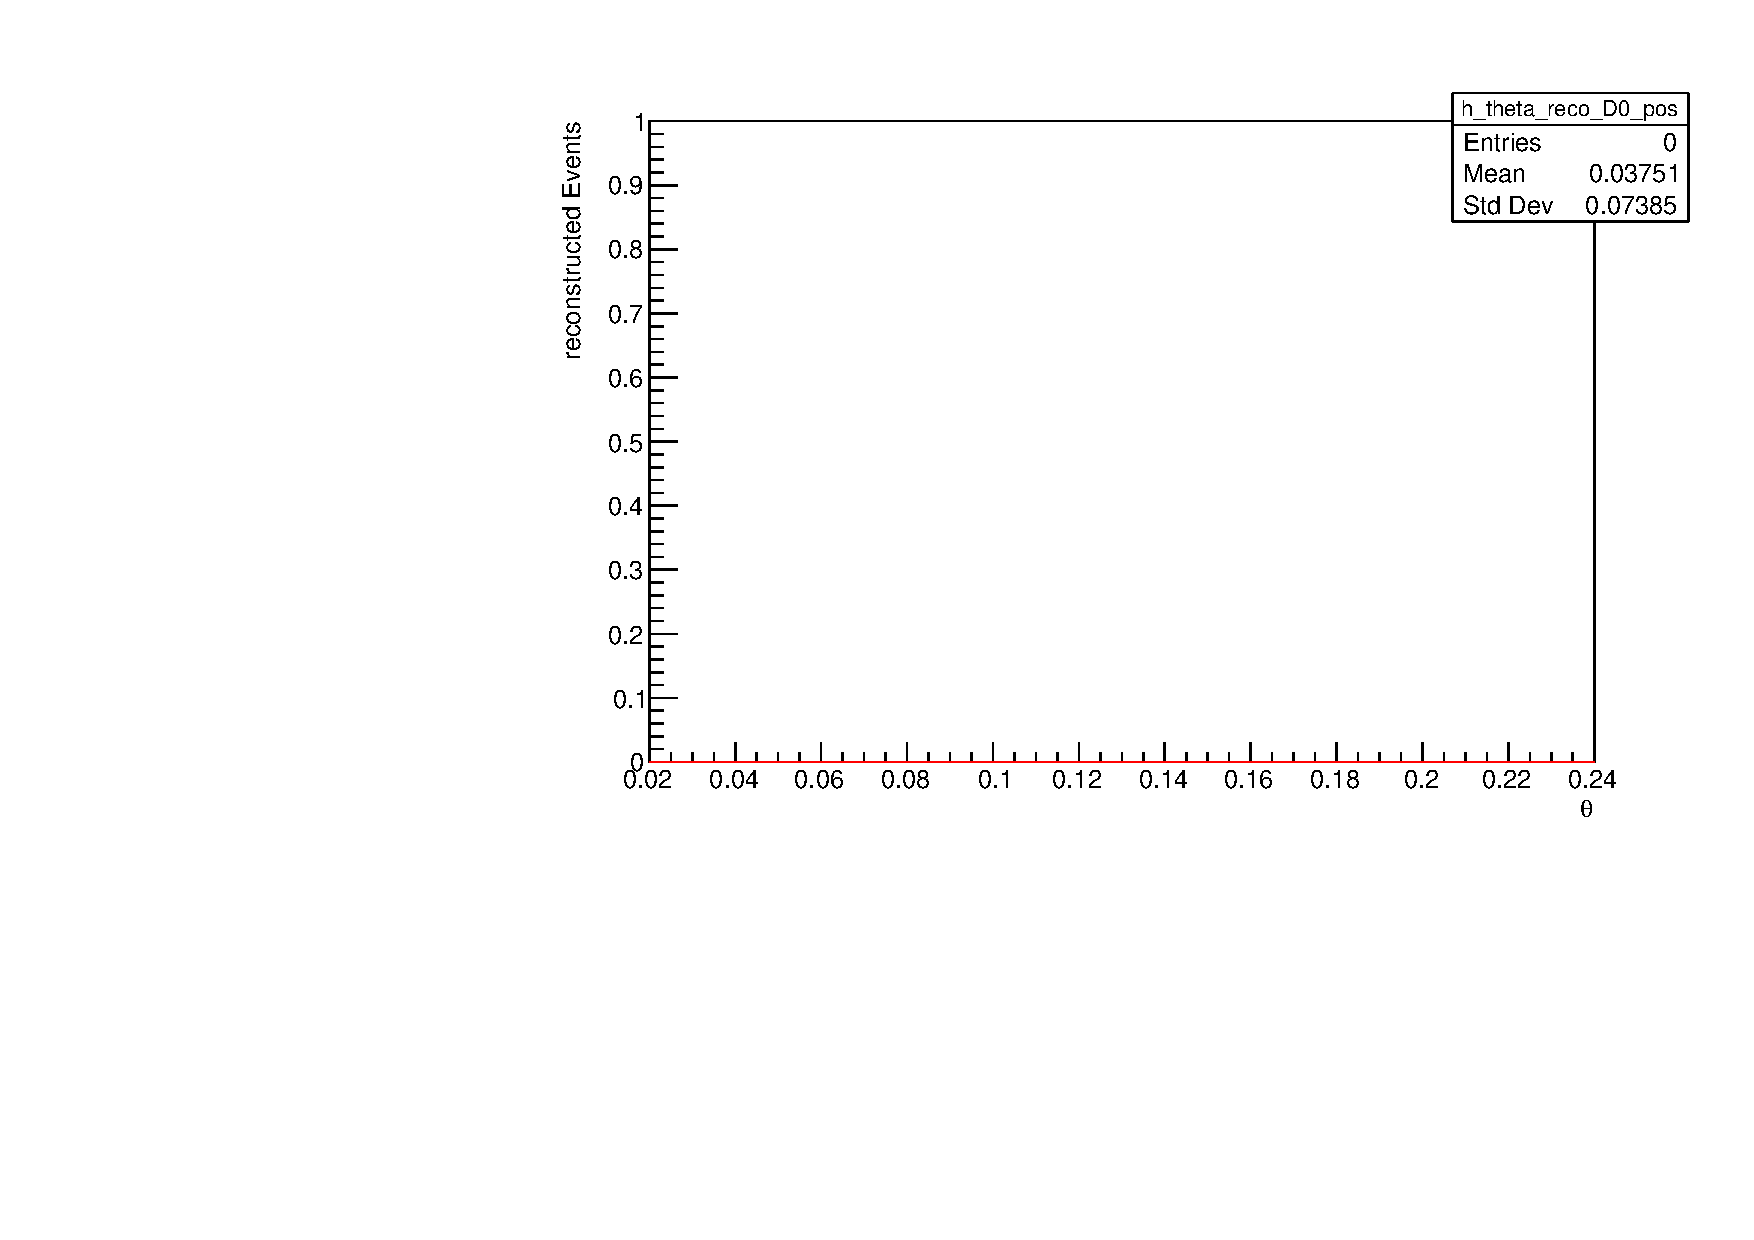
\includegraphics[width=0.9\textwidth]{up_pdf/single/pos/h_theta_reco_D0_pos.pdf}
\end{subfigure}
\begin{subfigure}{0.45\textwidth}
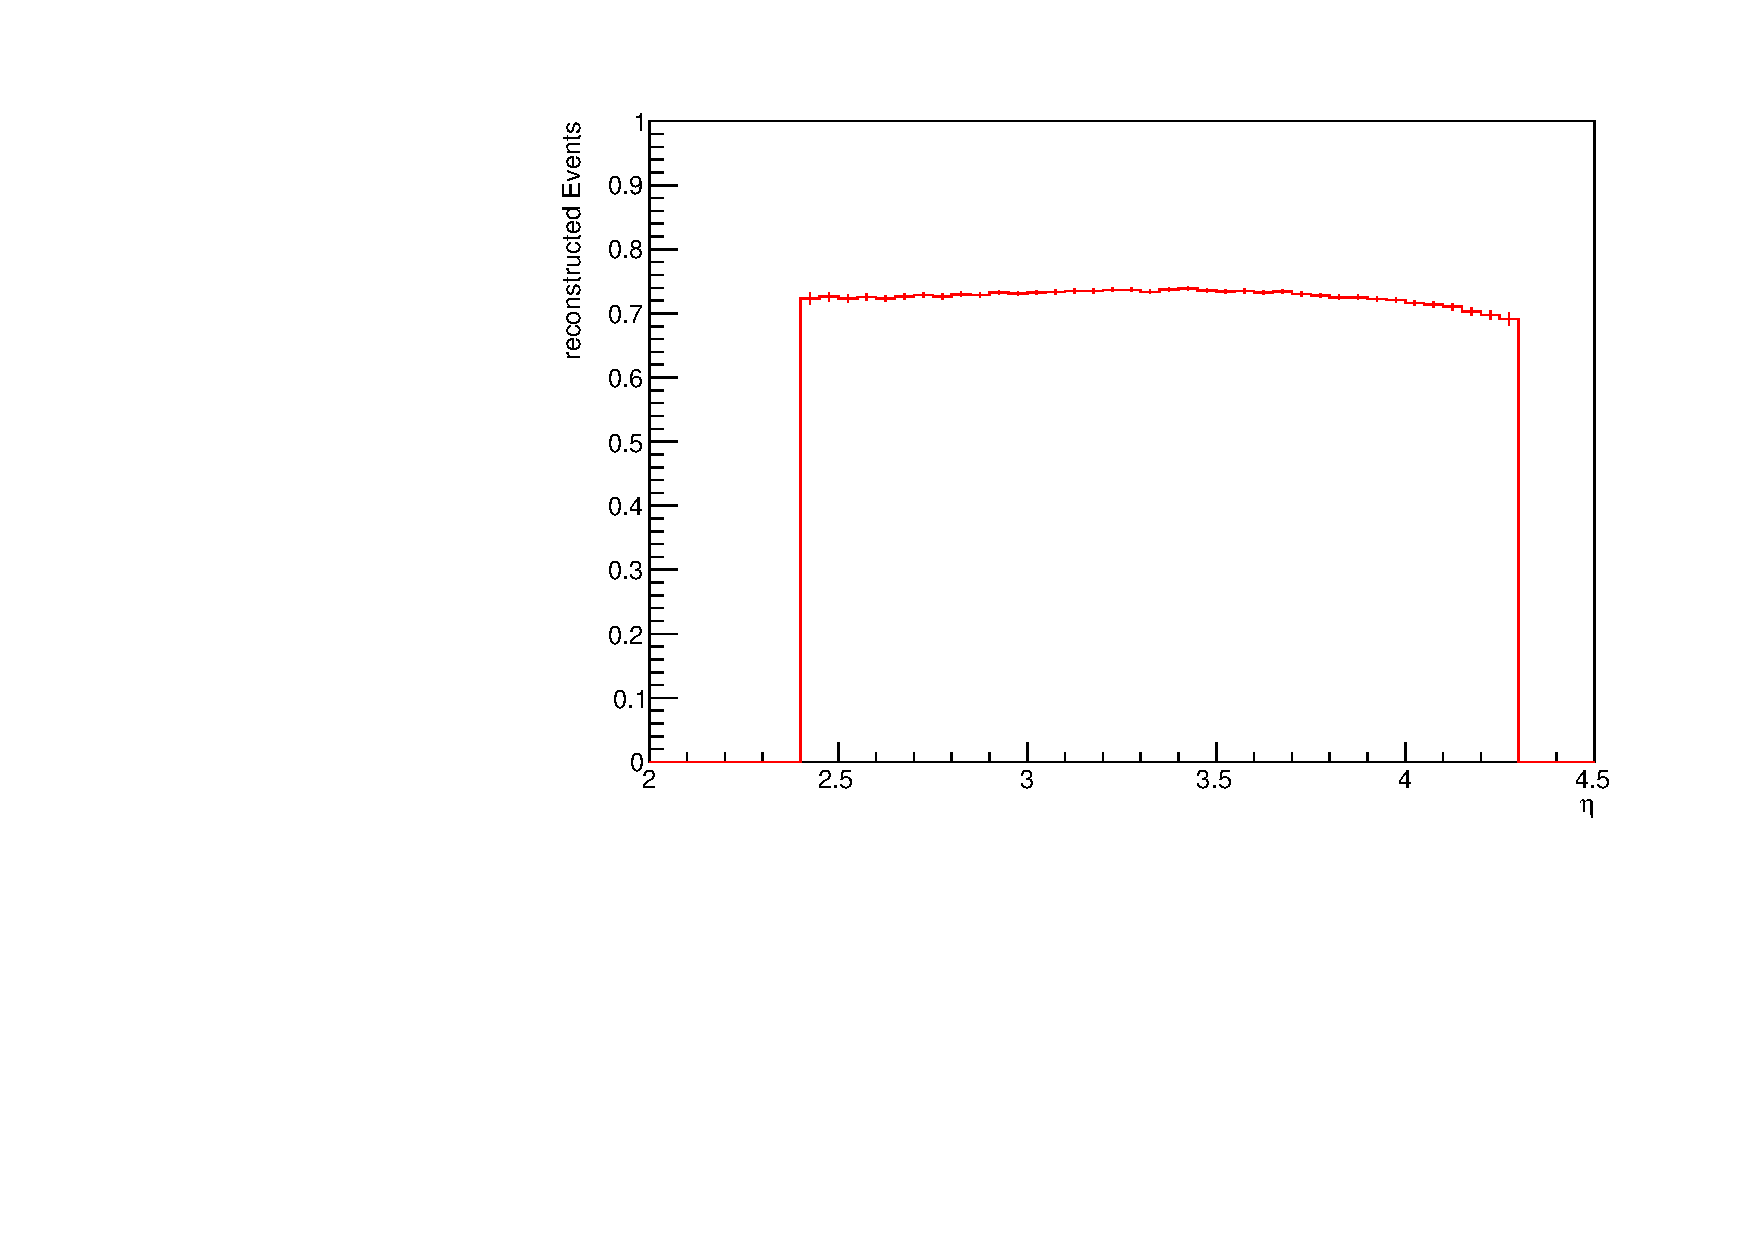
\includegraphics[width=0.9\textwidth]{up_pdf/single/pos/h_eta_reco_D0_pos.pdf}
\end{subfigure}
\end{figure}
\end{frame}
\begin{frame}{$D^*$-efficiency}
\begin{figure}
\begin{subfigure}{0.45\textwidth}
\includegraphics[width=0.9\textwidth]{up_pdf/single/pos/h_pt_reco_Dst_pos.pdf}
\end{subfigure}
\begin{subfigure}{0.45\textwidth}
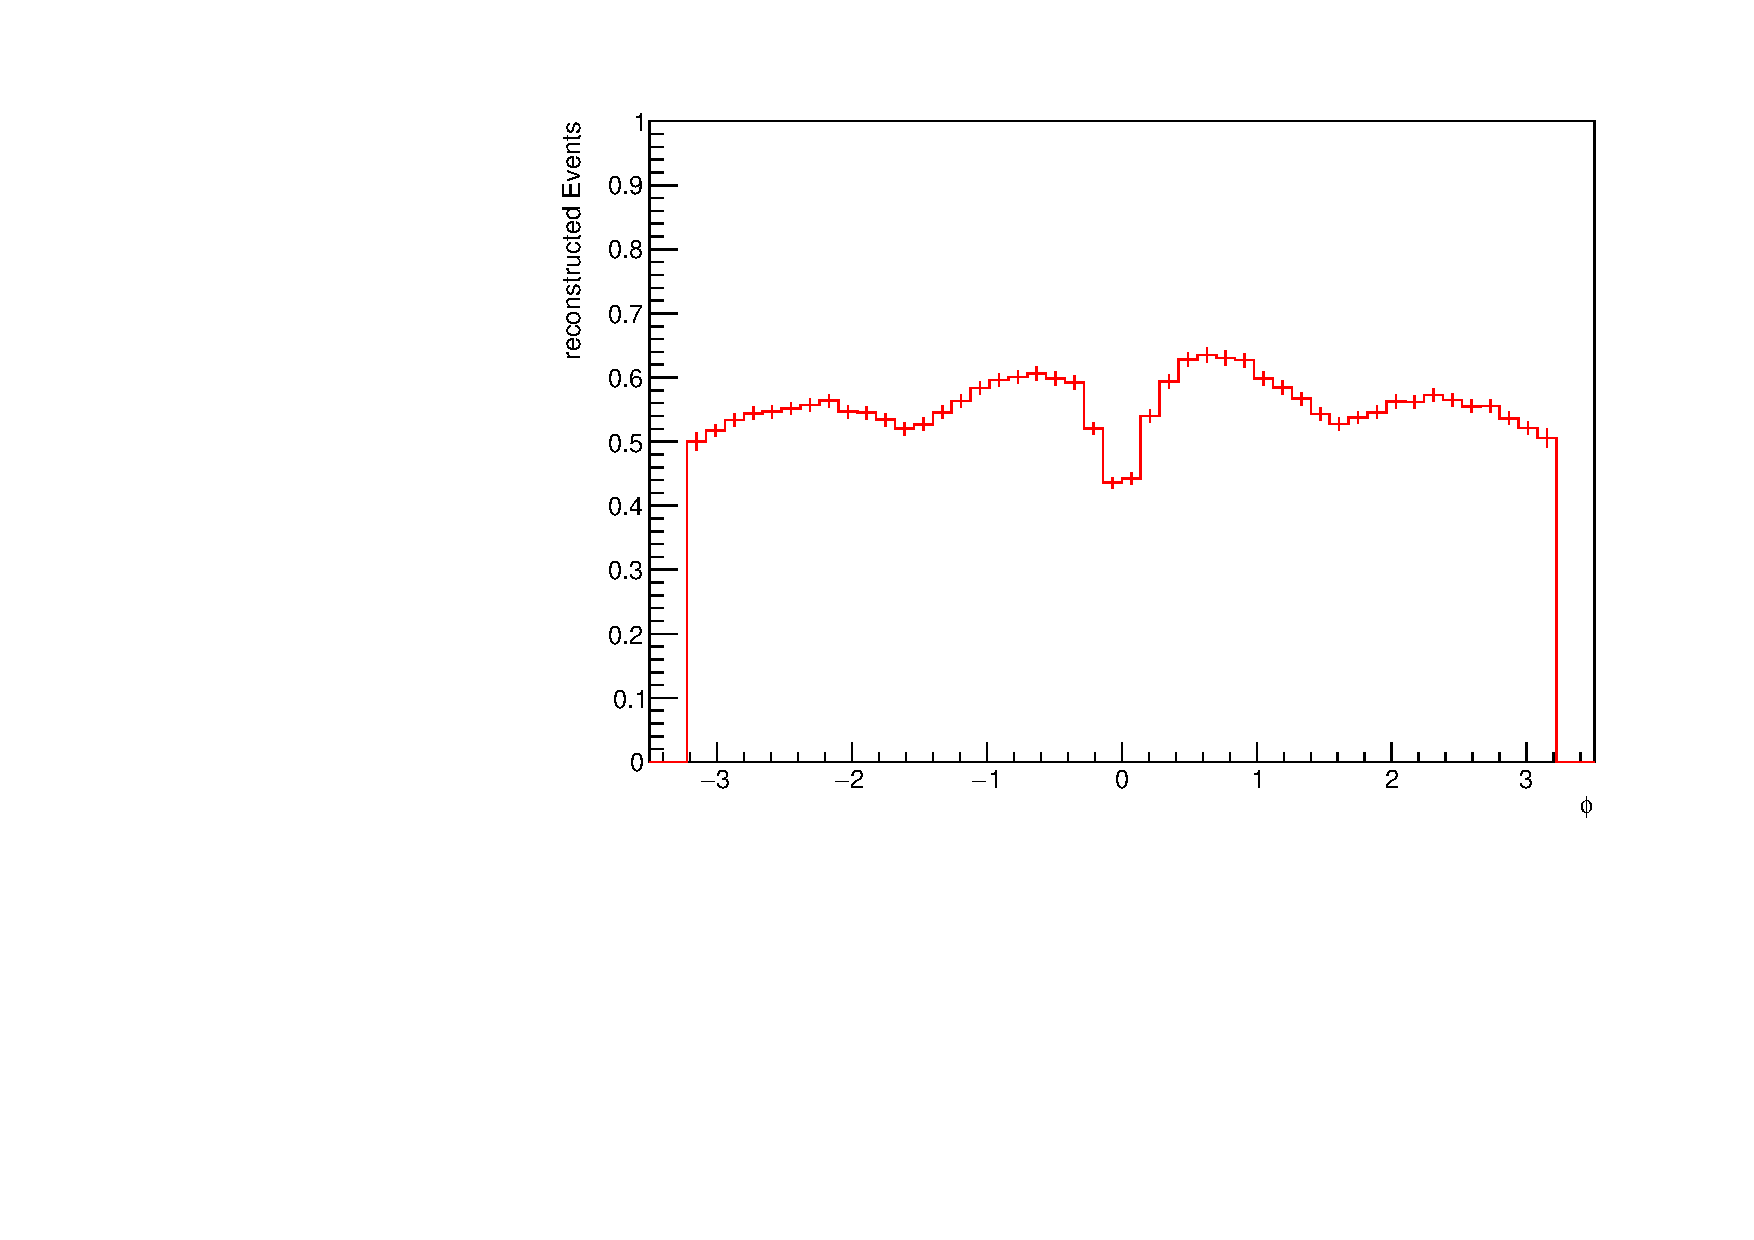
\includegraphics[width=0.9\textwidth]{up_pdf/single/pos/h_phi_reco_Dst_pos.pdf}
\end{subfigure}
\begin{subfigure}{0.45\textwidth}
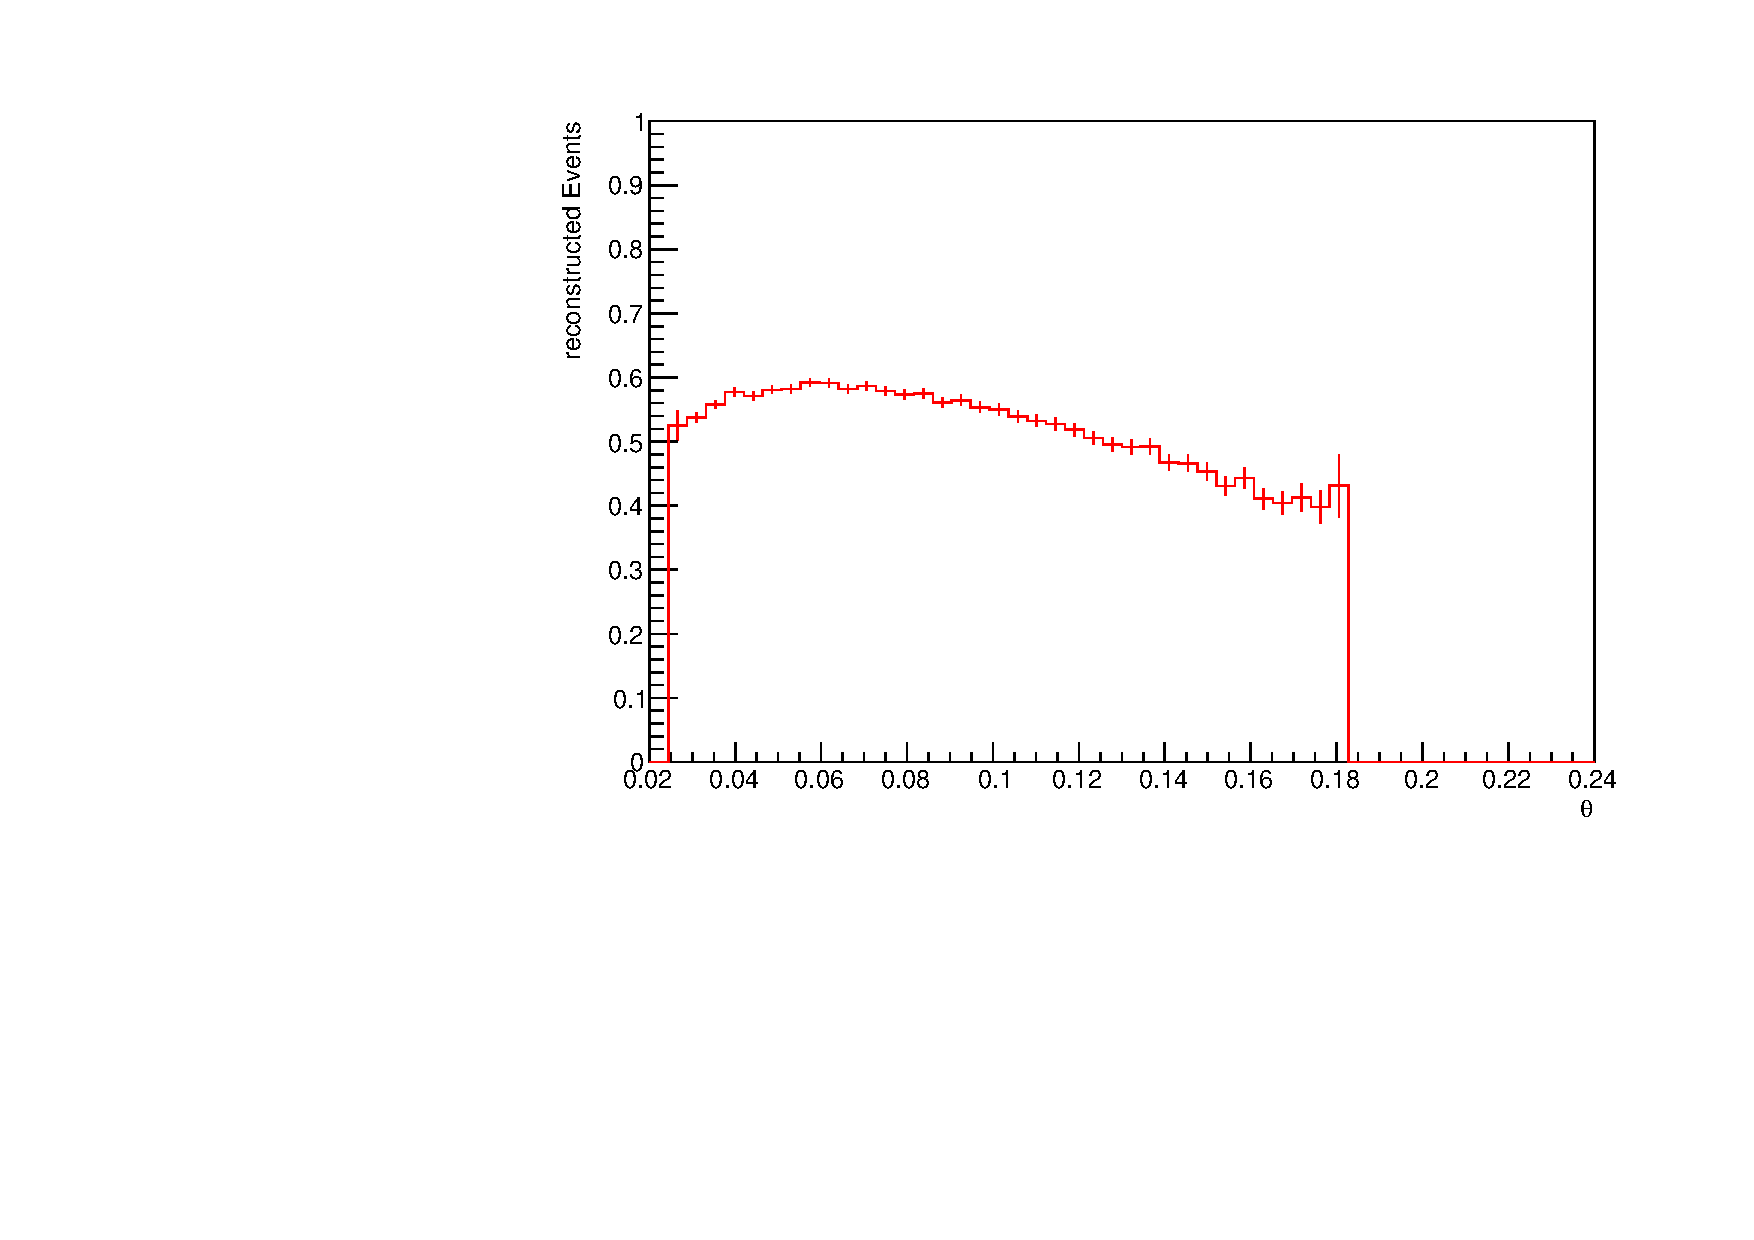
\includegraphics[width=0.9\textwidth]{up_pdf/single/pos/h_theta_reco_Dst_pos.pdf}
\end{subfigure}
\begin{subfigure}{0.45\textwidth}
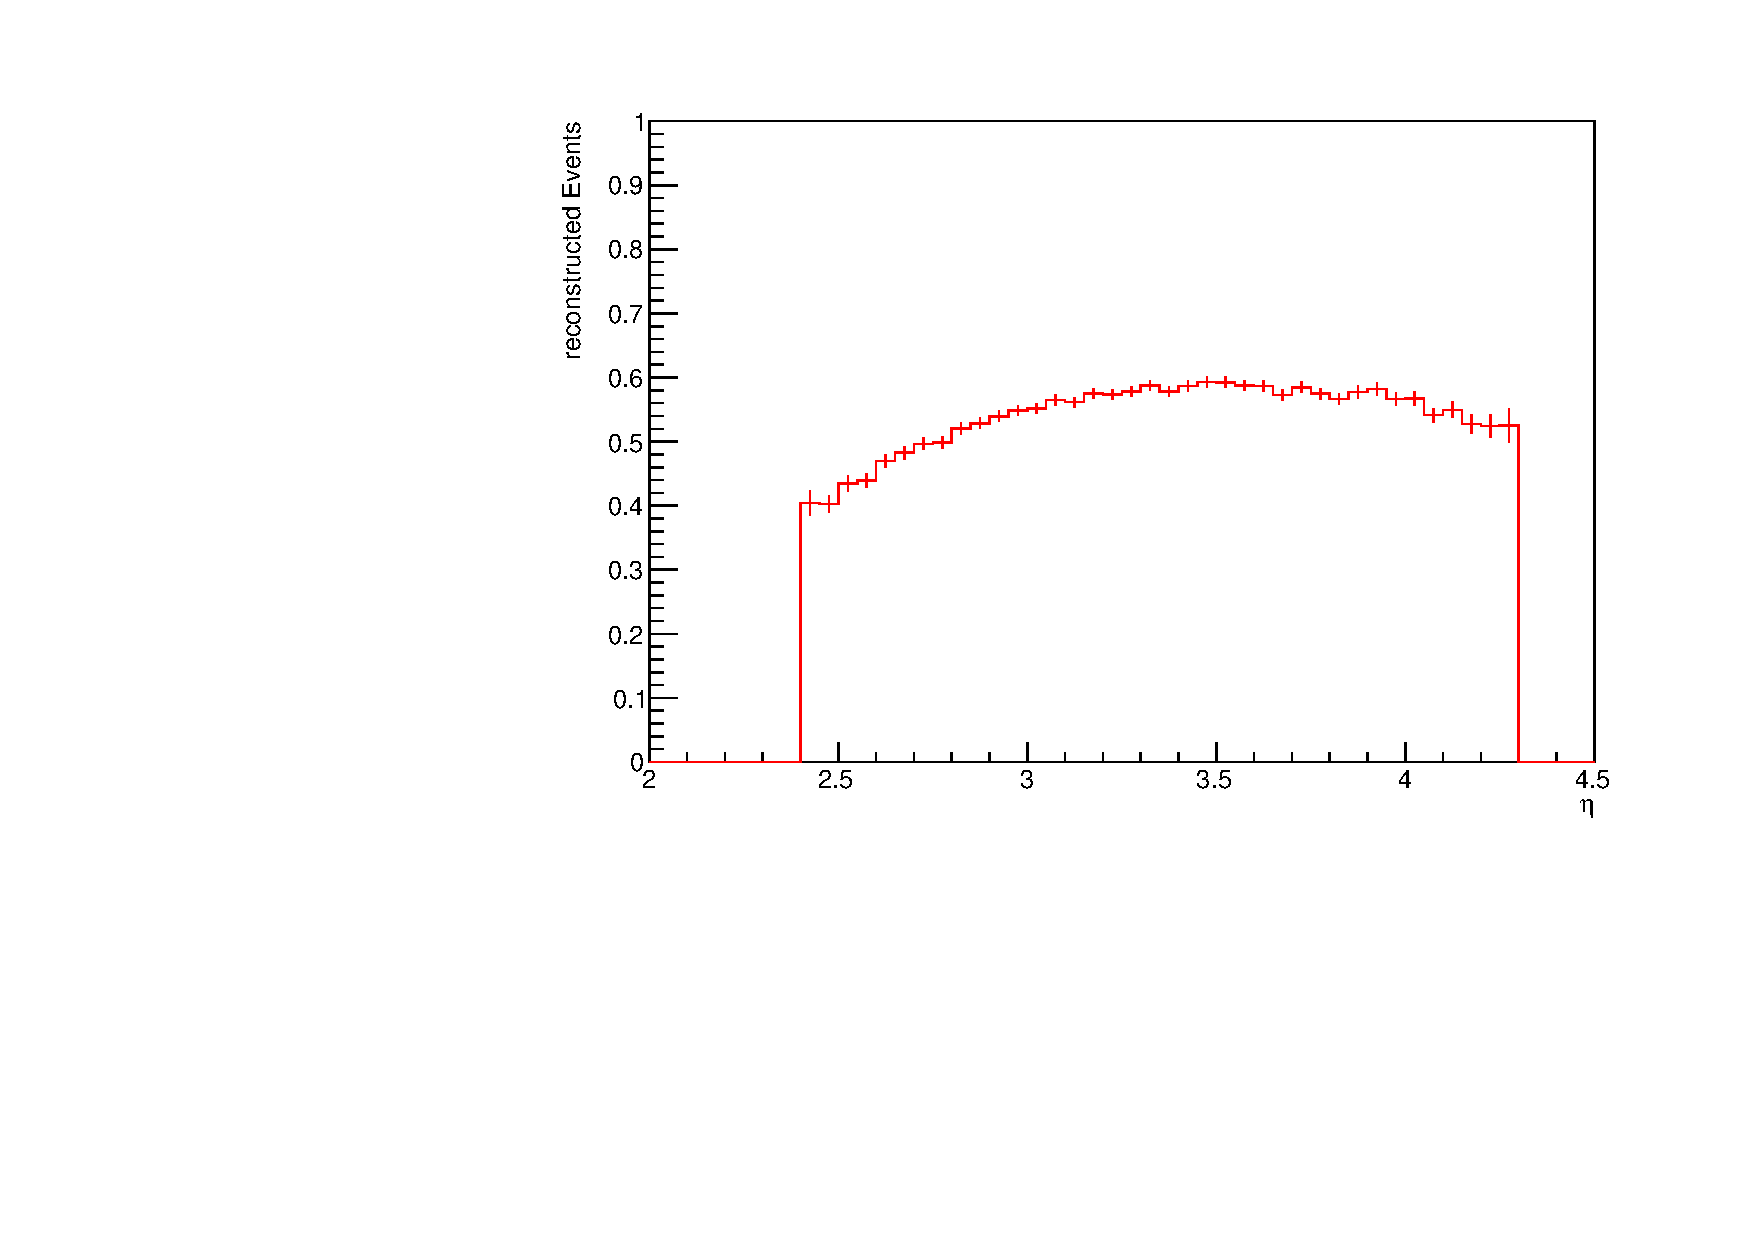
\includegraphics[width=0.9\textwidth]{up_pdf/single/pos/h_eta_reco_Dst_pos.pdf}
\end{subfigure}
\end{figure}
\end{frame}
\begin{frame}
\begin{LARGE}
\textbf{Charge: -}
\end{LARGE}
\end{frame}
\begin{frame}{Efficiencies}
\begin{table}
\resizebox{\textwidth}{!}{
	\begin{tabular}{cS[table-format=2.2]@{${}\pm{}$}S[table-format=1.2]S[table-format=2.2]@{${}\pm{}$}S[table-format=1.2]S[table-format=2.2]@{${}\pm{}$}S[table-format=1.2]S[table-format=2.2]@{${}\pm{}$}S[table-format=1.2]S[table-format=2.2]@{${}\pm{}$}S[table-format=1.2]}
		\toprule
		{Polarity} & \multicolumn{2}{c}{$\epsilon_{\pi} $} & \multicolumn{2}{c}{$\epsilon_{K} $} & \multicolumn{2}{c}{$ \epsilon_{\pi,s} $} & \multicolumn{2}{c}{$\epsilon_{D^0} $} & \multicolumn{2}{c}{$\epsilon_{D^*} $} \\
		\midrule
		$UP$ & 86.60 & 0.06 & 84.30 & 0.06 & 76.97 & 0.07 & 73.65 & 0.07 & 56.81 & 0.08 \\
		$DOWN$ & 86.64 & 0.06 & 83.95 & 0.07 & 76.36 & 0.07 & 73.74 & 0.08 & 56.38 & 0.09 \\
		\bottomrule
	\end{tabular}}
\end{table}
\end{frame}
\begin{frame}{$\pi$-efficiency}
\begin{figure}
\begin{subfigure}{0.45\textwidth}
\includegraphics[width=0.9\textwidth]{up_pdf/single/neg/h_pt_reco_Pi_neg.pdf}
\end{subfigure}
\begin{subfigure}{0.45\textwidth}
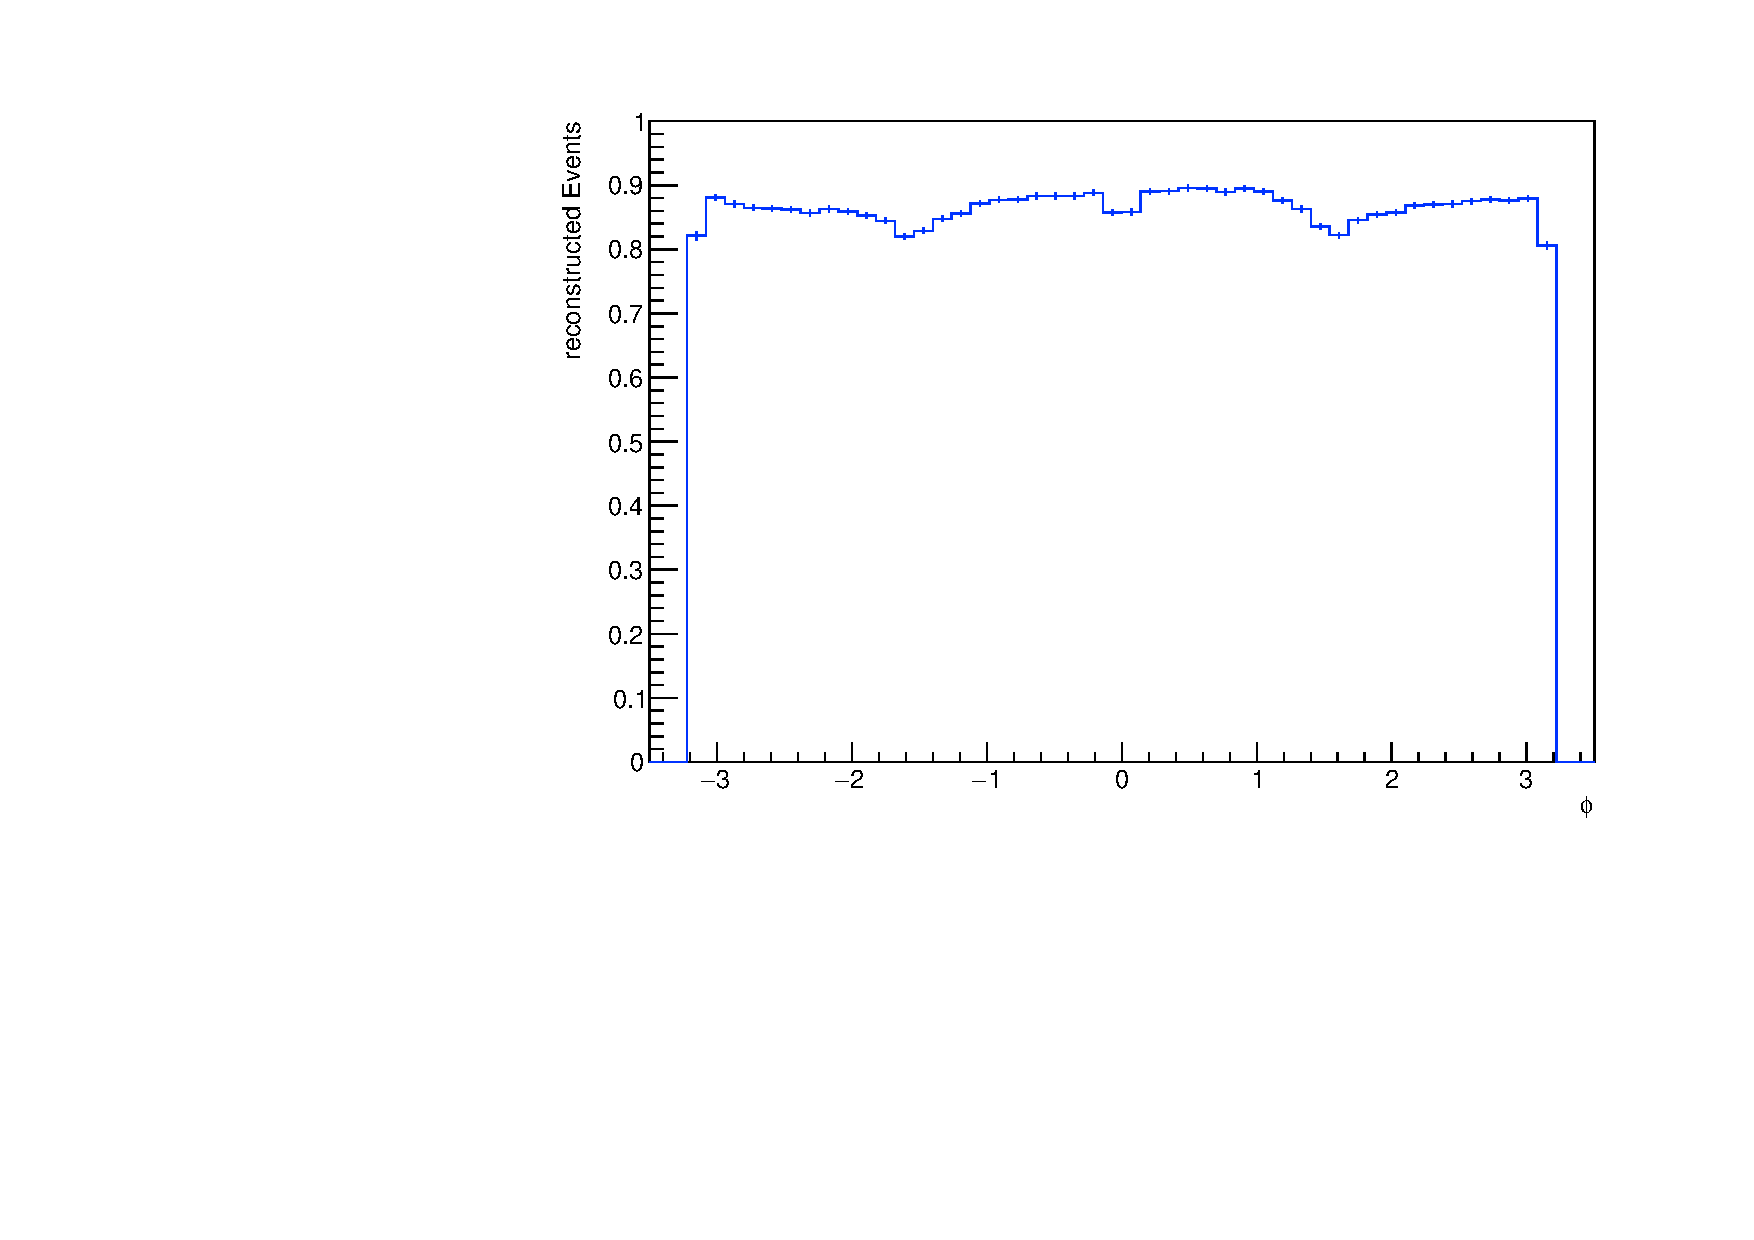
\includegraphics[width=0.9\textwidth]{up_pdf/single/neg/h_phi_reco_Pi_neg.pdf}
\end{subfigure}
\begin{subfigure}{0.45\textwidth}
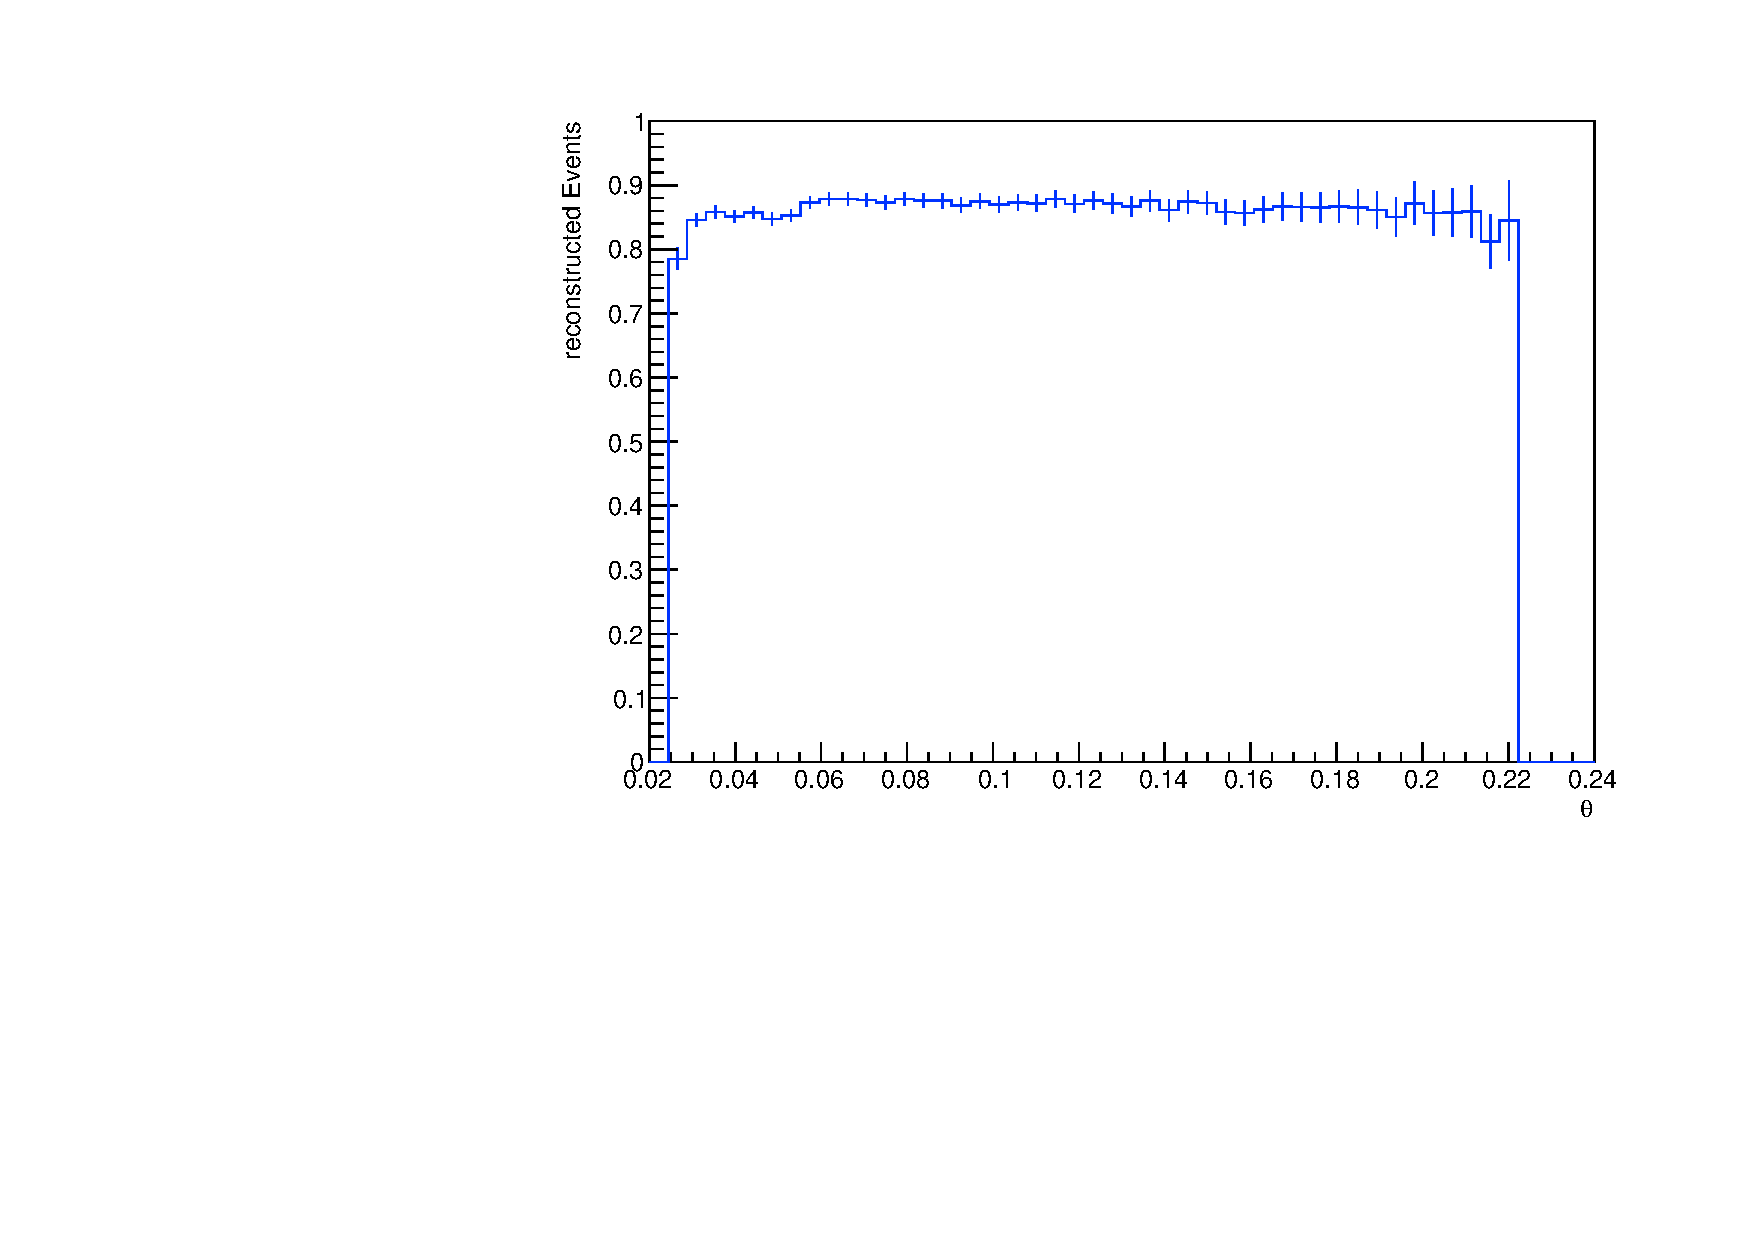
\includegraphics[width=0.9\textwidth]{up_pdf/single/neg/h_theta_reco_Pi_neg.pdf}
\end{subfigure}
\begin{subfigure}{0.45\textwidth}
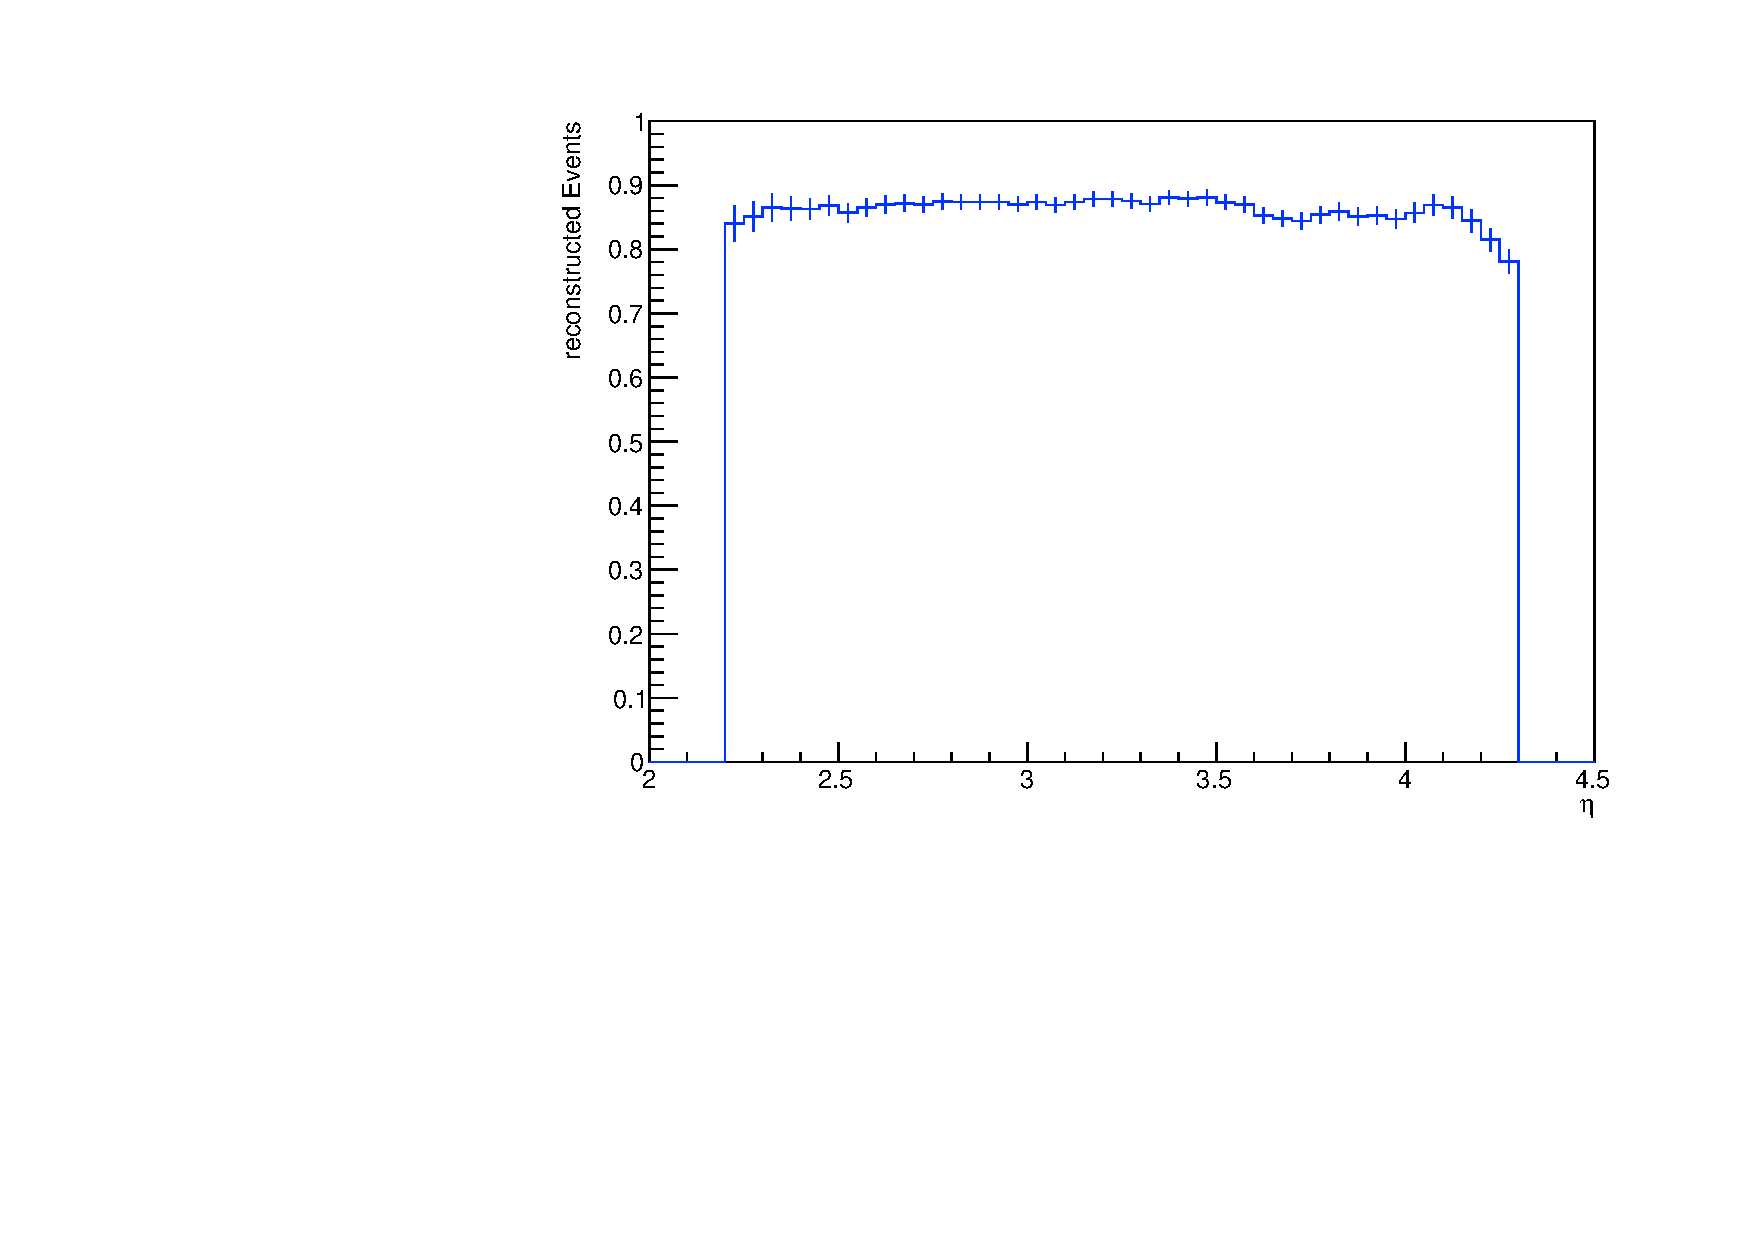
\includegraphics[width=0.9\textwidth]{up_pdf/single/neg/h_eta_reco_Pi_neg.pdf}
\end{subfigure}
\end{figure}
\end{frame}
\begin{frame}{$K$-efficiency}
\begin{figure}
\begin{subfigure}{0.45\textwidth}
\includegraphics[width=0.9\textwidth]{up_pdf/single/neg/h_pt_reco_K_neg.pdf}
\end{subfigure}
\begin{subfigure}{0.45\textwidth}
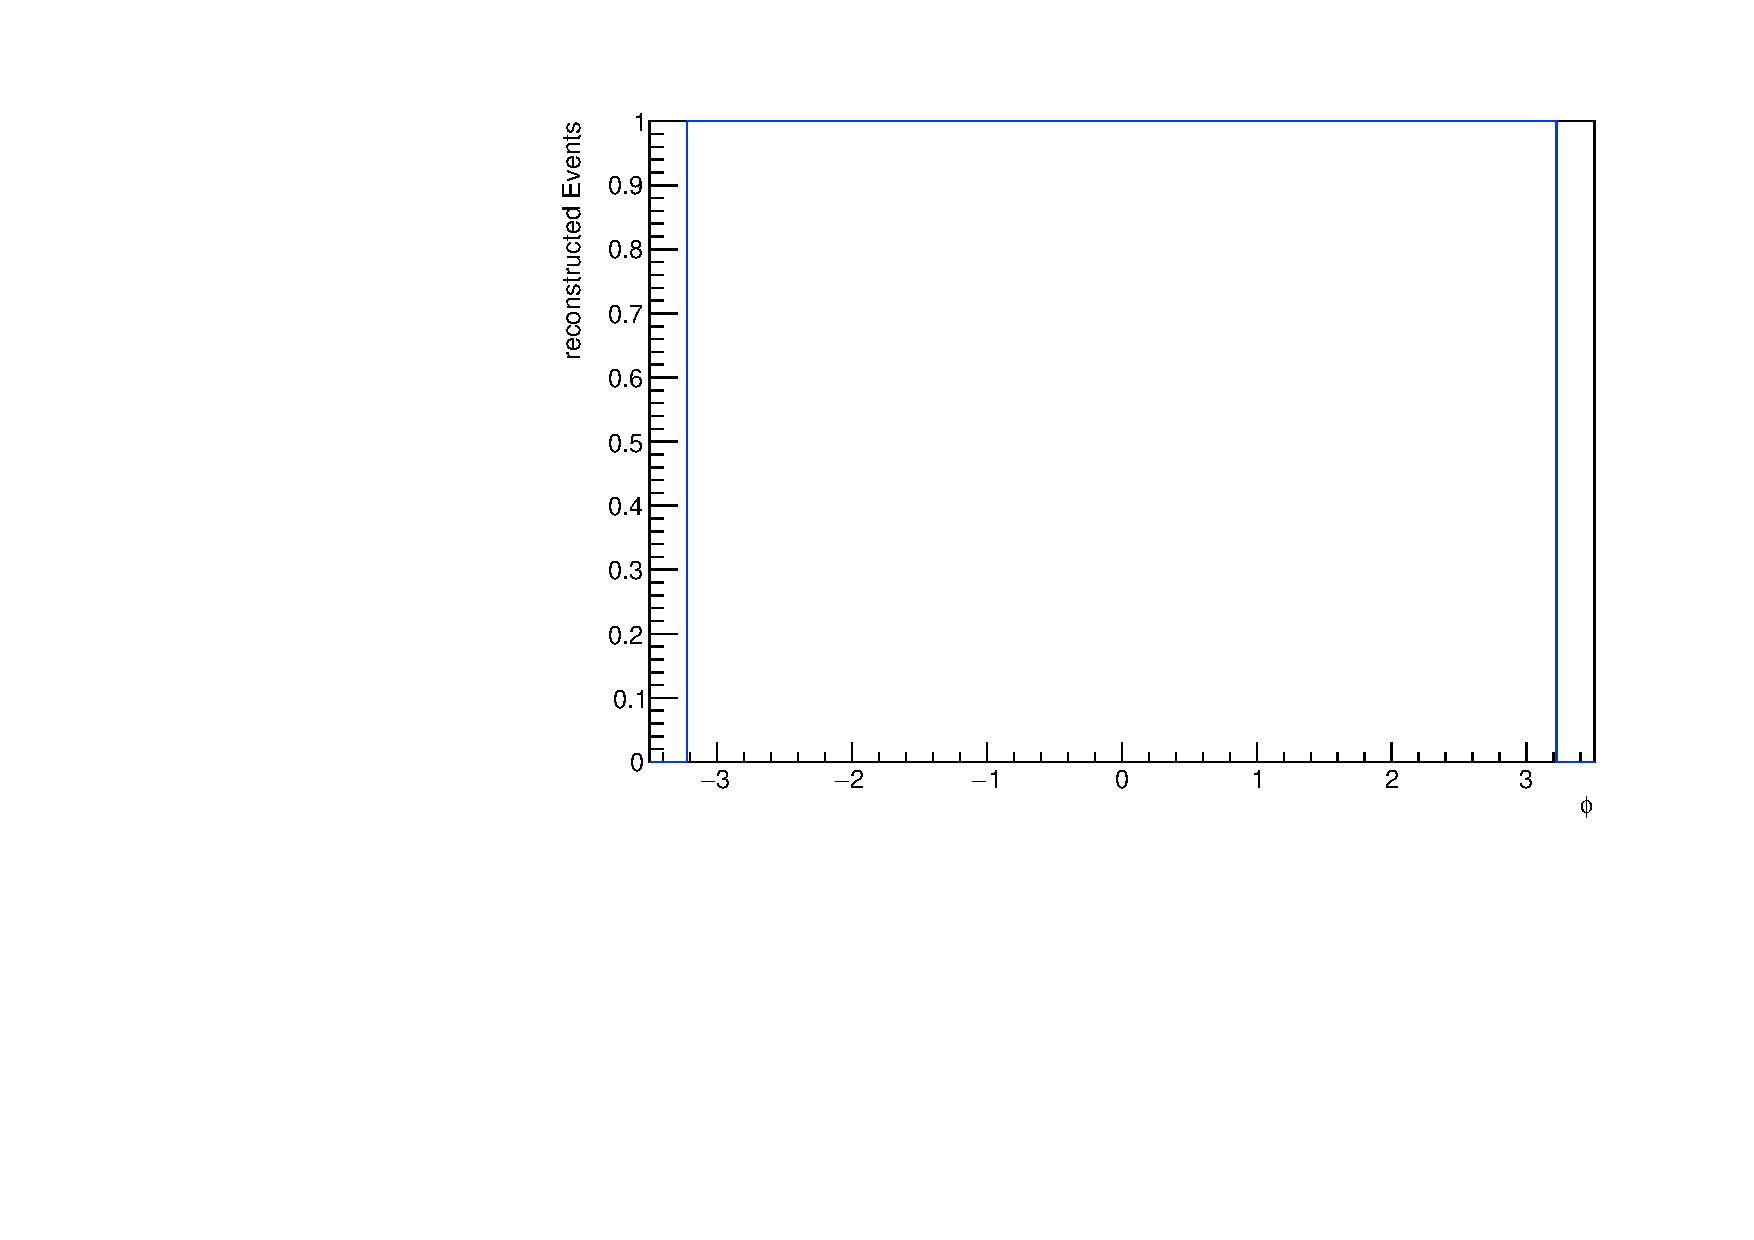
\includegraphics[width=0.9\textwidth]{up_pdf/single/neg/h_phi_reco_K_neg.pdf}
\end{subfigure}
\begin{subfigure}{0.45\textwidth}
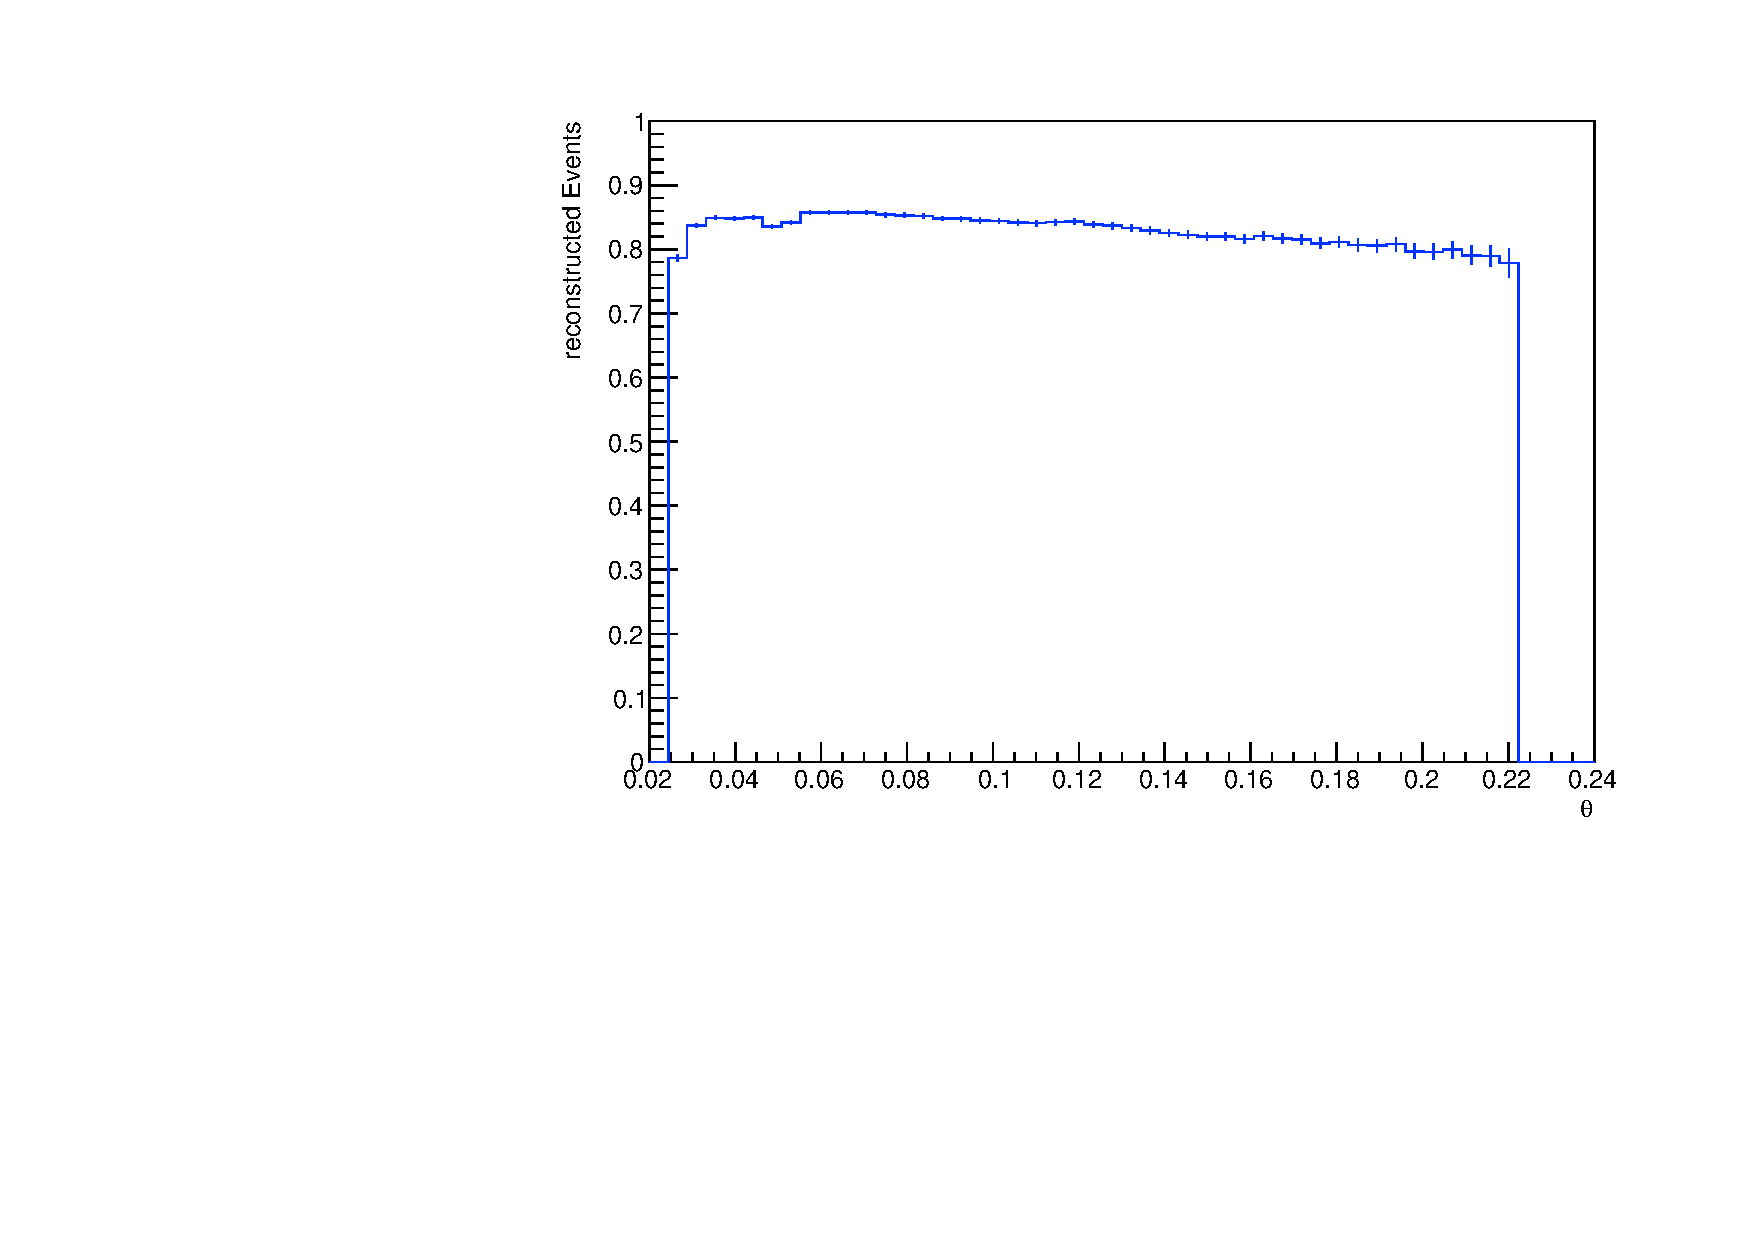
\includegraphics[width=0.9\textwidth]{up_pdf/single/neg/h_theta_reco_K_neg.pdf}
\end{subfigure}
\begin{subfigure}{0.45\textwidth}
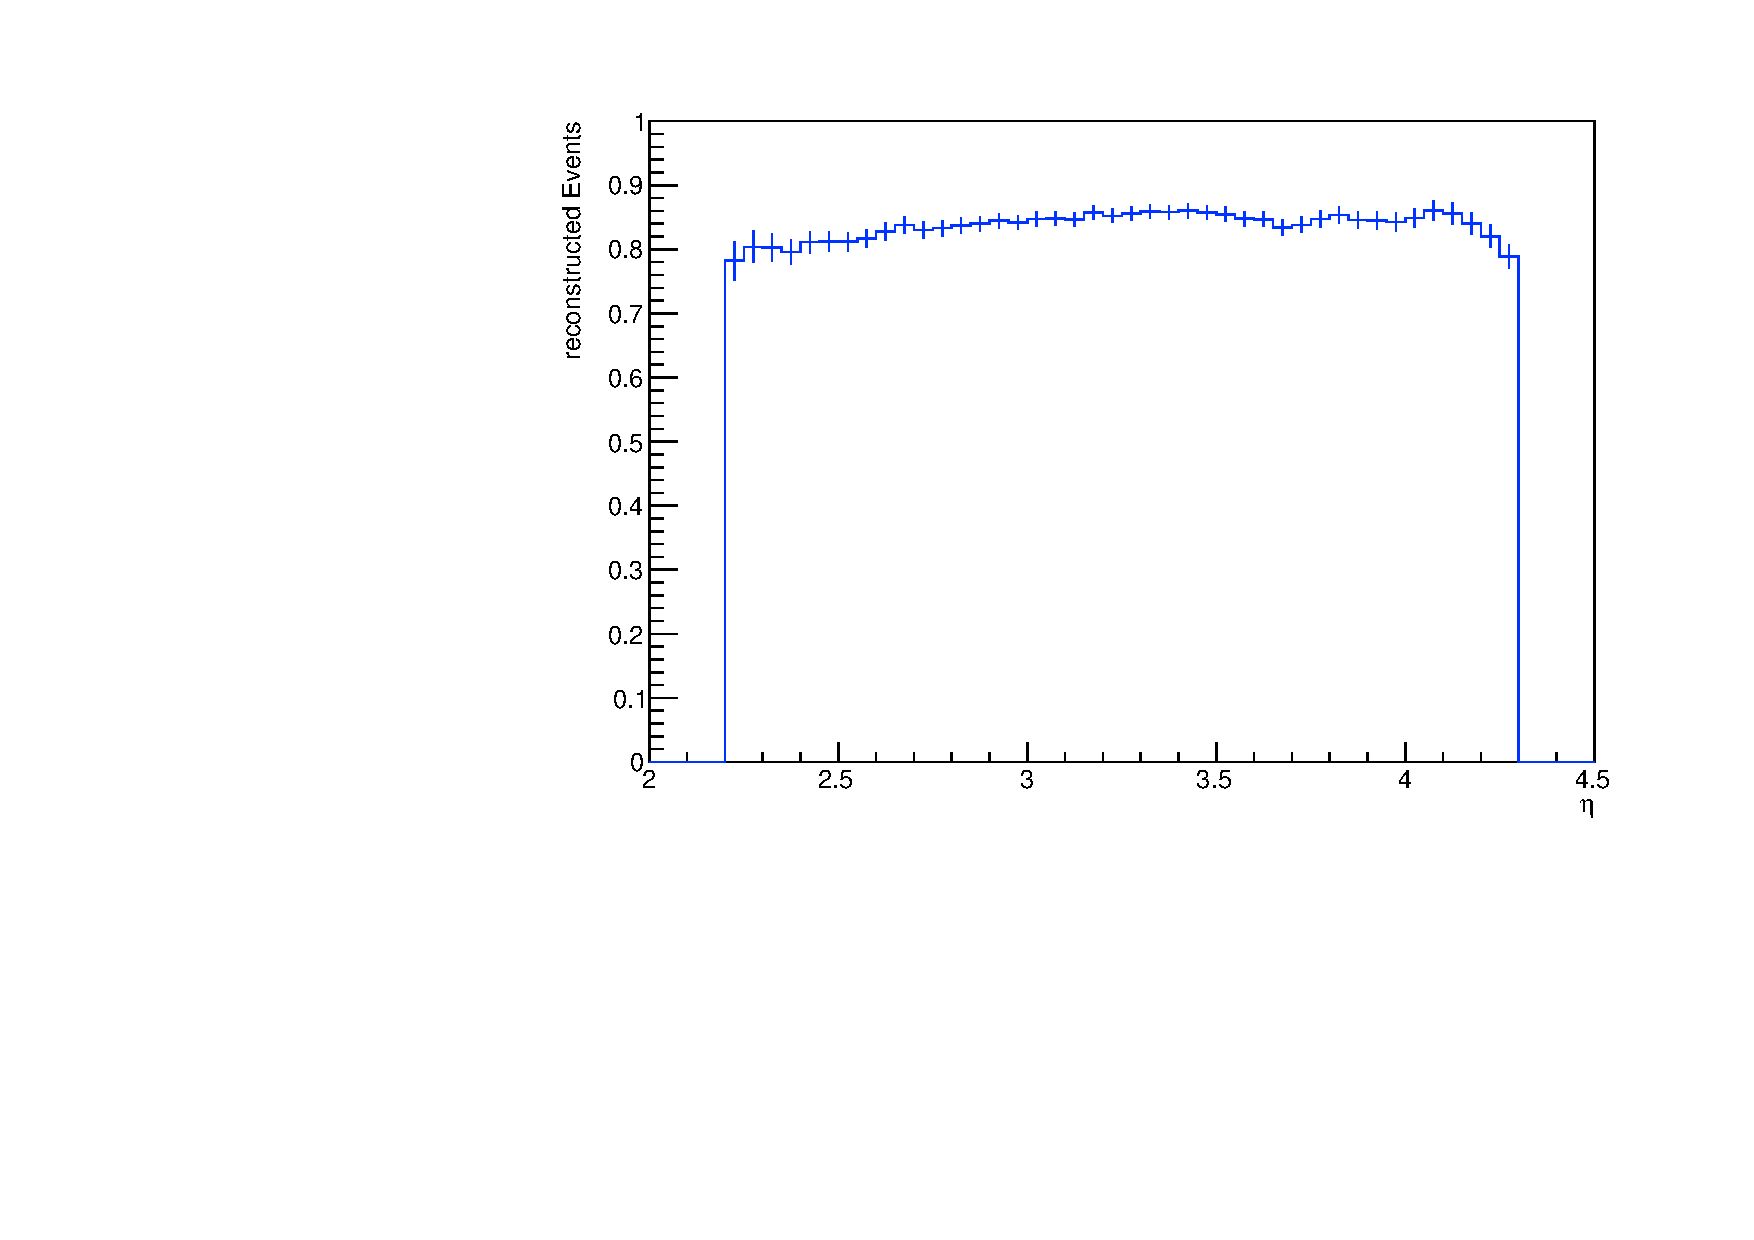
\includegraphics[width=0.9\textwidth]{up_pdf/single/neg/h_eta_reco_K_neg.pdf}
\end{subfigure}
\end{figure}
\end{frame}
\begin{frame}{soft $\pi$-efficiency}
\begin{figure}
\begin{subfigure}{0.45\textwidth}
\includegraphics[width=0.9\textwidth]{up_pdf/single/neg/h_pt_reco_SPi_neg.pdf}
\end{subfigure}
\begin{subfigure}{0.45\textwidth}
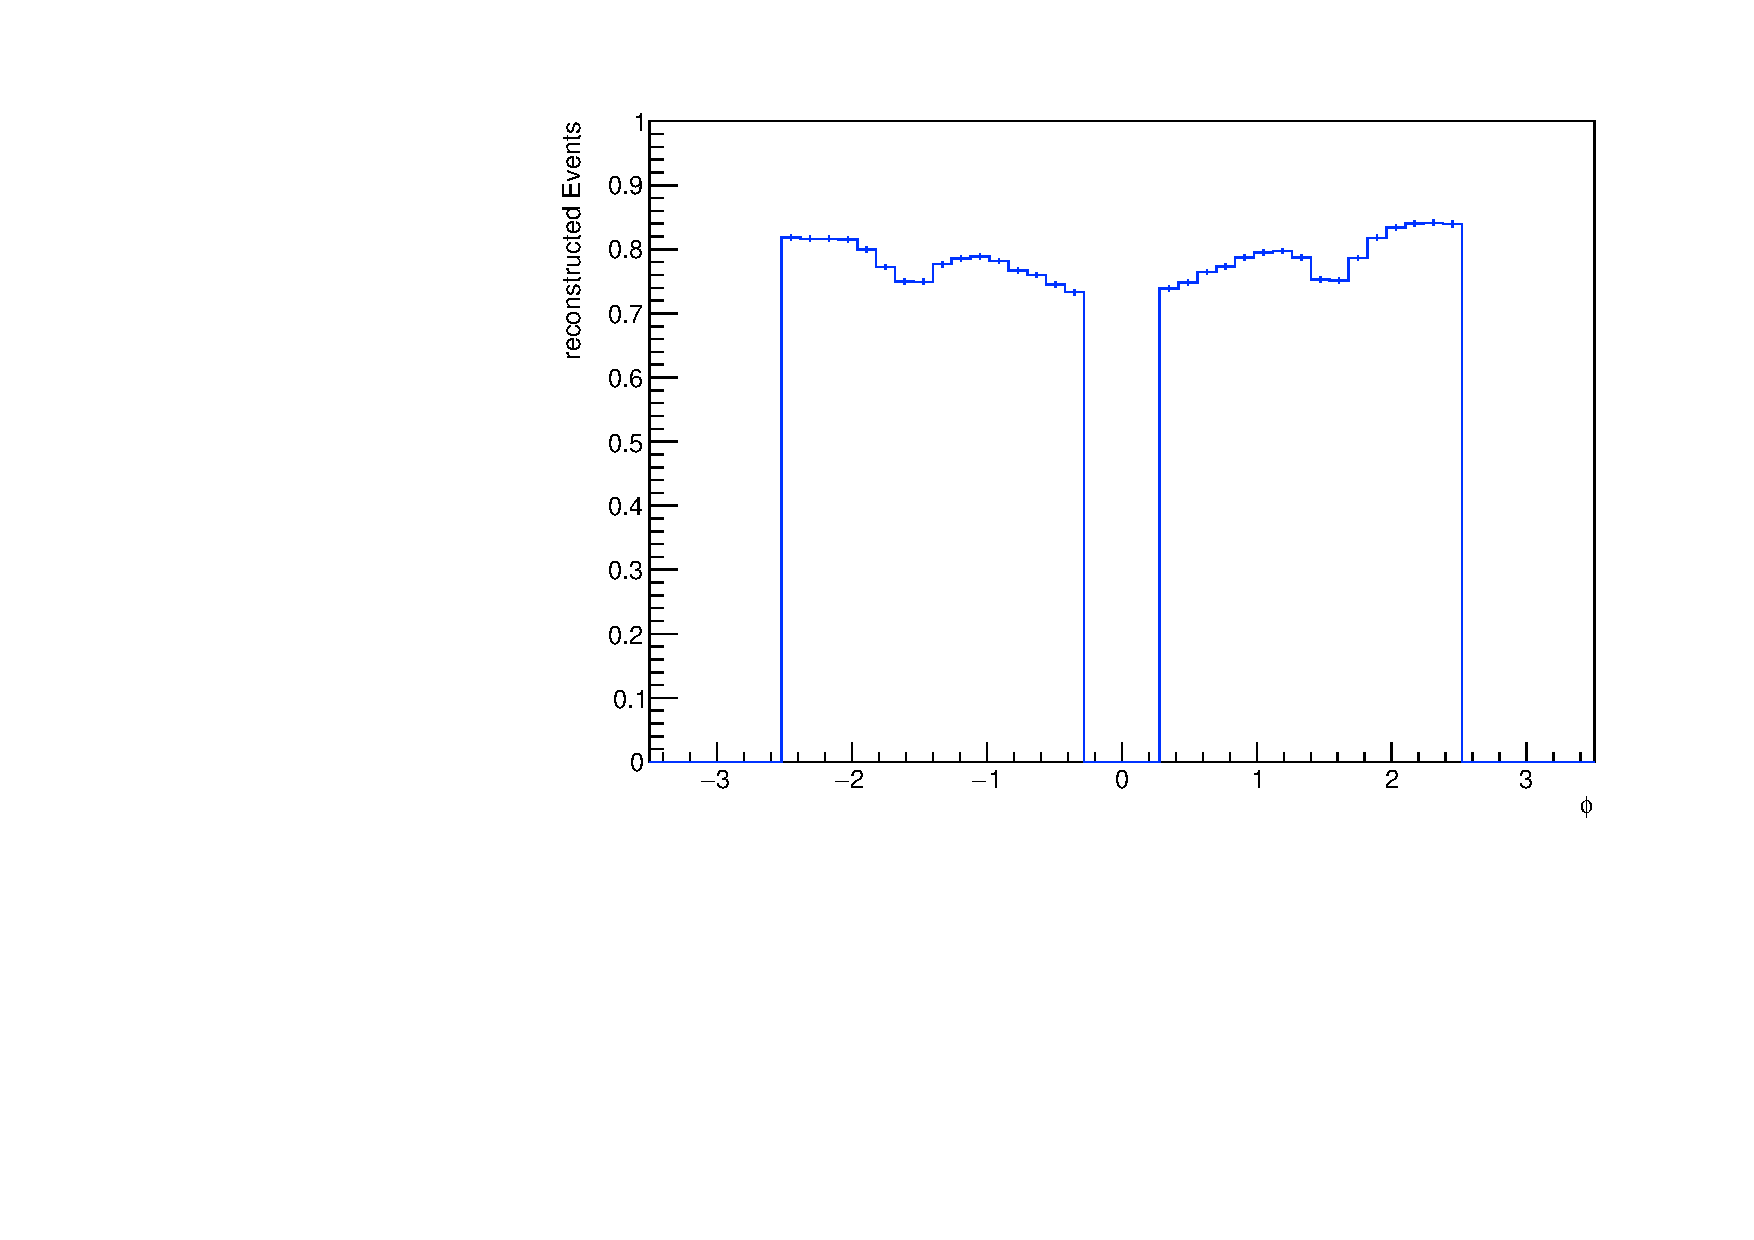
\includegraphics[width=0.9\textwidth]{up_pdf/single/neg/h_phi_reco_SPi_neg.pdf}
\end{subfigure}
\begin{subfigure}{0.45\textwidth}
\includegraphics[width=0.9\textwidth]{up_pdf/single/neg/h_theta_reco_SPi_neg.pdf}
\end{subfigure}
\begin{subfigure}{0.45\textwidth}
\includegraphics[width=0.9\textwidth]{up_pdf/single/neg/h_eta_reco_SPi_neg.pdf}
\end{subfigure}
\end{figure}
\end{frame}
\begin{frame}{$D^0$-efficiency}
\begin{figure}
\begin{subfigure}{0.45\textwidth}
\includegraphics[width=0.9\textwidth]{up_pdf/single/neg/h_pt_reco_D0_neg.pdf}
\end{subfigure}
\begin{subfigure}{0.45\textwidth}
\includegraphics[width=0.9\textwidth]{up_pdf/single/neg/h_phi_reco_D0_neg.pdf}
\end{subfigure}
\begin{subfigure}{0.45\textwidth}
\includegraphics[width=0.9\textwidth]{up_pdf/single/neg/h_theta_reco_D0_neg.pdf}
\end{subfigure}
\begin{subfigure}{0.45\textwidth}
\includegraphics[width=0.9\textwidth]{up_pdf/single/neg/h_eta_reco_D0_neg.pdf}
\end{subfigure}
\end{figure}
\end{frame}
\begin{frame}{$D^*$-efficiency}
\begin{figure}
\begin{subfigure}{0.45\textwidth}
\includegraphics[width=0.9\textwidth]{up_pdf/single/neg/h_pt_reco_Dst_neg.pdf}
\end{subfigure}
\begin{subfigure}{0.45\textwidth}
\includegraphics[width=0.9\textwidth]{up_pdf/single/neg/h_phi_reco_Dst_neg.pdf}
\end{subfigure}
\begin{subfigure}{0.45\textwidth}
\includegraphics[width=0.9\textwidth]{up_pdf/single/neg/h_theta_reco_Dst_neg.pdf}
\end{subfigure}
\begin{subfigure}{0.45\textwidth}
\includegraphics[width=0.9\textwidth]{up_pdf/single/neg/h_eta_reco_Dst_neg.pdf}
\end{subfigure}
\end{figure}
\end{frame}
\begin{frame}{Deviation}
\begin{table}
	\caption{The deviation $\frac{\epsilon_+ - \epsilon_-}{\epsilon_+ + \epsilon_-}/10^{-3}$}
	\resizebox{\textwidth}{!}{
	\begin{tabular}{cS[table-format=1.1]@{${}\pm{}$}S[table-format=1.1]S[table-format=1.1]@{${}\pm{}$}S[table-format=1.1]S[table-format=1.1]@{${}\pm{}$}S[table-format=1.1]S[table-format=1.1]@{${}\pm{}$}S[table-format=1.1]S[table-format=1.1]@{${}\pm{}$}S[table-format=1.1]}
		\toprule
		{Polarity} & \multicolumn{2}{c}{$\pi $} & \multicolumn{2}{c}{$ K $} & \multicolumn{2}{c}{$ soft \pi $} & \multicolumn{2}{c}{$ D^0 $} & \multicolumn{2}{c}{$ D^* $} \\
		\midrule
		$UP$ & 0.2 & 0.8 & 4.0 & 0.8 & -5.0 & 1.0 & -4.0 & 1.0 & -9.8 & 1.1 \\
		$DOWN$ & -0.4 & 0.9 & 8.0 & 0.9 & 2.3 & 1.1 & -6.0 & 1.2 & -2.5 & 1.3\\
		\bottomrule
	\end{tabular}}
\end{table}
\end{frame}
\begin{frame}{Comparison of different charges - $D^*$}
\begin{figure}
\begin{subfigure}{0.45\textwidth}
\includegraphics[width=0.9\textwidth]{up_pdf/combined/h_pt_reco_Dst.pdf}
\end{subfigure}
\begin{subfigure}{0.45\textwidth}
\includegraphics[width=0.9\textwidth]{up_pdf/combined/h_phi_reco_Dst.pdf}
\end{subfigure}
\begin{subfigure}{0.45\textwidth}
\includegraphics[width=0.9\textwidth]{up_pdf/combined/h_theta_reco_Dst.pdf}
\end{subfigure}
\begin{subfigure}{0.45\textwidth}
\includegraphics[width=0.9\textwidth]{up_pdf/combined/h_eta_reco_Dst.pdf}
\end{subfigure}
\end{figure}
\end{frame}
\begin{frame}{Comparison - $D^* p_\text{T}$}
\centering
\includegraphics[width=0.9\textwidth]{up_pdf/combined/h_pt_reco_Dst.pdf}
\end{frame}
\begin{frame}{Comparison - $D^* \phi$}
\centering
\includegraphics[width=0.9\textwidth]{up_pdf/combined/h_phi_reco_Dst.pdf}
\end{frame}
\begin{frame}{Comparison - $D^* \theta$}
\centering
\includegraphics[width=0.9\textwidth]{up_pdf/combined/h_theta_reco_Dst.pdf}
\end{frame}
\begin{frame}{Comparison - $D^* \eta$}
\centering
\includegraphics[width=0.9\textwidth]{up_pdf/combined/h_eta_reco_Dst.pdf}
\end{frame}
\begin{frame}{$D^*$ deviation dependencies}
\begin{figure}
\begin{subfigure}{0.45\textwidth}
\includegraphics[width=0.9\textwidth]{up_pdf/deviation/h_pt_reco_Dst_pos.pdf}
\end{subfigure}
\begin{subfigure}{0.45\textwidth}
\includegraphics[width=0.9\textwidth]{up_pdf/deviation/h_phi_reco_Dst_pos.pdf}
\end{subfigure}
\begin{subfigure}{0.45\textwidth}
\includegraphics[width=0.9\textwidth]{up_pdf/deviation/h_theta_reco_Dst_pos.pdf}
\end{subfigure}
\begin{subfigure}{0.45\textwidth}
\includegraphics[width=0.9\textwidth]{up_pdf/deviation/h_eta_reco_Dst_pos.pdf}
\end{subfigure}
\end{figure}
\end{frame}
\begin{frame}{$D^*$ deviation - $\phi$}
\includegraphics[width=0.9\textwidth]{up_pdf/deviation/h_phi_reco_Dst_pos.pdf}
\end{frame}
\end{document}


%♥